\documentclass[english,12pt,a4paper, reqno,
draft,
final,
 titlepage]{amsbook}

\linespread{1.5}

\usepackage{master}


\title[Temporal Dynamics in Generative Models]{Temporal Dynamics in Generative Models.}

\hypersetup{pdftitle={Temporal Dynamics in Generative Models},
pdfauthor={Maren Hackenberg}}
\graphicspath{{Figures/}}

\fancypagestyle{plain}{%
\fancyhf{} % clear all header and footer fields
\fancyhead[RO, LE]{\thepage}
\fancyhead[LO, RE]{Temporal Dynamics in Generative Models.}%Title
\renewcommand{\headrulewidth}{0.4pt}
\renewcommand{\footrulewidth}{0pt}
\renewcommand{\headheight}{14pt}
}

\begin{document}

\frontmatter

%Title
\begin{titlepage}
\begin{center}
\begin{figure}[]
% \begin{center}

\includegraphics[width=0.65\textwidth]{logo.pdf}
% \end{center}
\end{figure}
\vspace{0.3cm}                  

{\LARGE Temporal Dynamics in Generative Models}
\vspace{2.0cm}

Masterarbeit im Studiengang Master of Science in Mathematik

verfasst von

{\large Maren~Hackenberg} \vspace{1cm}

am Mathematischen Institut der Fakultät für Mathematik und Physik

an der Albert-Ludwigs-Universität Freiburg \vspace{1cm}

unter Anleitung von 

{\large Prof.~Dr.~Harald~Binder}



\end{center}
\end{titlepage}

\blankpage

%Acknowledgements
\setcounter{page}{1}

\pagestyle{plain}

\chapter*{Acknowledgement}

First and foremost, I thank Harald Binder for his invaluable support and encouragement, for introducing me to a fascinating field of research and giving me the opportunity to write this thesis, and for never running out of good ideas. 

Also, I am very grateful to Peter Pfaffelhuber for co-supervising this thesis. 

I thoroughly appreciate the positive and supportive atmosphere at the IMBI and feel honoured to have met and worked with such fantastic colleagues.
In particular, I would like to thank the members of the AG Machine Learning: 
Caroline Broichhagen, Daniela Zöller, Göran Köber, Kiana Farhadyar, Martin Treppner, Moritz Hess and Stefan Lenz. 

Considering myself extremely lucky to have friends both very supportive and skilled in mathematics and statistics, I am deeply grateful to Anselm Hudde, Maja von Cube, Nora Scherer and Pascal Schlosser for the time they took to discuss and proofread this thesis and for all their helpful comments. 

My final thanks go to my brother Paul, who so generously helped me out with the necessary hardware, to my parents Anke and Thomas and to Anselm for always standing behind me and for unconditionally and unfailingly believing in me. 


% Table of contents
\renewcommand{\baselinestretch}{1.45}\normalsize
\tableofcontents
\renewcommand{\baselinestretch}{1.5}\normalsize

% Main text body
\mainmatter
\pagestyle{plain}

\chapter{Introduction}\label{chap:intro}
\fancyhead[LO]{\nouppercase{\leftmark}}

When considering biomedical time-series data from individuals, understanding and capturing the underlying development patterns on an individual level is the first and essential step towards personalised medicine. Yet, such data are often characterised by a sparse, highly irregular time grid of measurements and individual-specific development patterns, which complicates the corresponding modelling task. 

In this thesis, I develop a generative deep learning model that infers individual-specific dynamics in a low-dimensional latent representation as solutions of ordinary differential equations (ODEs) from sparse and irregularly observed time-series data. The method is inspired by recent advances on combining black-box deep learning with explicit mechanistic modelling by differential equations and motivated by a scenario from the German National Cohort (NAKO) epidemiologic study.

Specifically, I simulate a data scenario based on a NAKO sub study: For each individual, an extensive characterisation with measurements of many variables is made at a baseline time point. To assess the level of measurement error in the data, a smaller subset of these variables is measured again at a second time point that is different for all individuals, i.e., the time spans between first and second measurement vary. Consequently, the data reflects individual-specific dynamic processes that are observed sparsely and irregularly with measurement noise. My aim is to develop a model that extracts underlying individual development patterns in such a setting despite the measurement uncertainty and the sparsity (only two time points) and irregularity of the time grid. Here, this irregular grid can potentially enable modelling of more complex dynamics by combining measurements of similar individuals.

\begin{figure}
	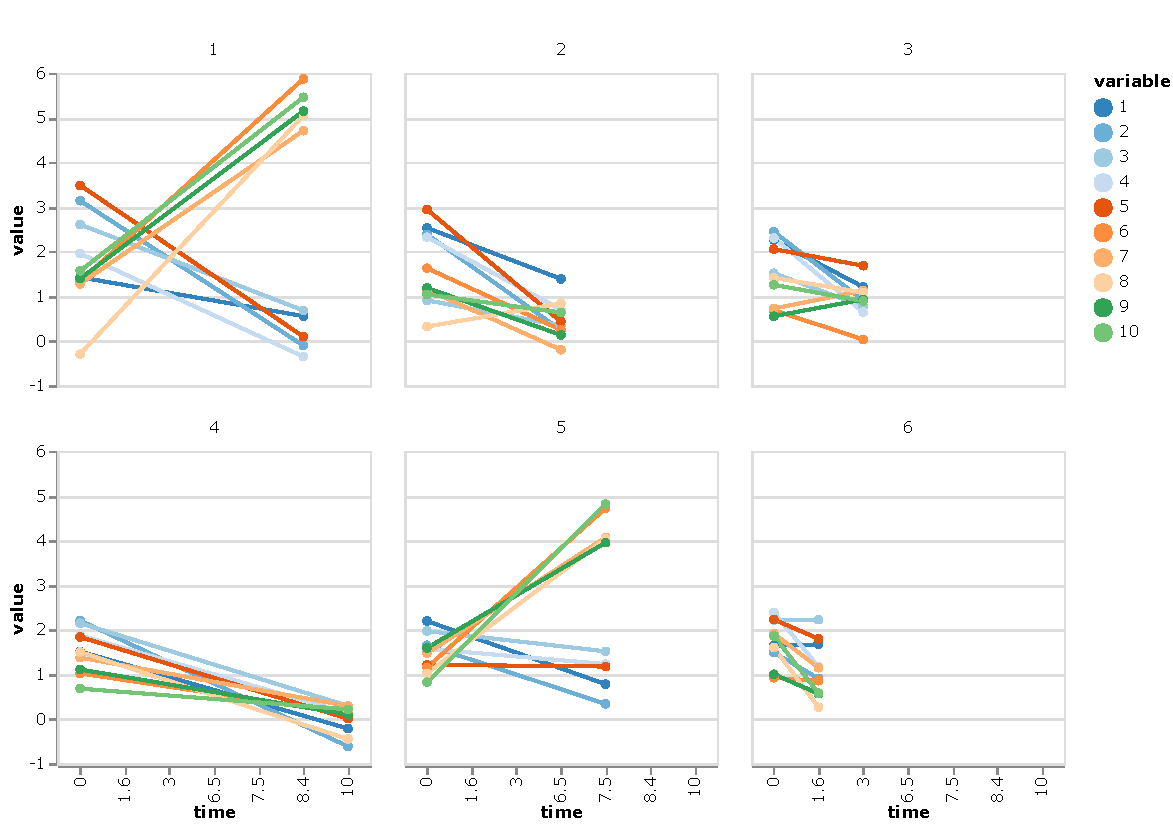
\includegraphics[width=0.8\linewidth]{exemplary_datastructure_intro.pdf}
	\caption{Exemplary data structure from simulated data. Each panel represents one individual, dots represent individual measurements and colors indicate different variables. The $x$-axis denotes the time of measurements and the $y$-axis their values.}
	\label{fig:exemplary-data}
\end{figure}

Figure \ref{fig:exemplary-data} illustrates the structure of the simulated data setting: The time point of the second measurement varies as contrasted by individuals $1$ and $6$. 
Different development patterns are reflected by two groups of individuals, one with an upward trend in some variables and a downward trend in others (e.g., individuals $1$ and $5$), and the other one with a downward trend in all the variables (e.g., individuals $2$ and $4$). 
Furthermore, the observations are characterised by groups of variables that share common trends, suggesting an underlying lower-dimensional structure. 

To build a representation of this lower-dimensional structure of the development patterns and in this way recover the central factors of variation underlying the data in an unsupervised way, I employ deep learning, specifically a variational autoencoder (VAE). I adapt the VAE and constrain its representation of the data in a latent space to model smooth trajectories by imposing an ODE system on that space. 
Furthermore, I assume inter-individual differences in development patterns to be grounded in differences in the variables measured only at baseline and use them to infer an individual-specific set of ODE parameters. 
To be able to model more complex underlying dynamics, I extend the model and enrich every individual's information by assigning to it a batch of individuals with similar underlying development patterns. The combination of all second time point measurements in the batch then serves as proxy information on the common dynamics at multiple time points. By training the model on these batches, I thus exploit the irregularity of second measurement time points to address the problem of time sparsity. 

Using the simulated data described above, I investigate the capability of the model to recover individual trajectories from both linear and non-linear two-dimensional ODE systems with two or four unknown parameters and to infer for a given observation a group of individuals with similar trajectories.

The proposed method is based on the central idea of bringing together deep learning and differential equations. This can be seen as an approach that bridges the gap between what has been referred to as the "two cultures in the use of statistical modeling to reach conclusions from data" (\cite[p.~1]{Breiman2001}): While inferring a low-dimensional latent representation in an unsupervised way directly from the data without specific assumptions on its structure with a deep neural network belongs to the "algorithmic modelling culture", the assumption of an explicit data model in the form of an underlying system of differential equations from which observations are generated with some random measurement noise represents the "data modelling culture".     

In general, formulating explicit scientific models allows to explicitly encode known structures of the data-generating forces such as physical laws or constraints into the model and treat other factors as noise, while the black-box nature of deep neural networks generally lacks interpretability. However, explicit stochastic or mechanistic data models make simplifying assumptions on the generating process that often cannot be validated. Algorithmic approaches such as neural networks have been successfully applied in many domains to approximate complex functions or learn patterns from data in an unsupervised way without explicit assumptions on the underlying data-generating process, but require large amounts of training data. 

Instead of viewing these two approaches to statistical modelling as opposing each other, recent lines of research attempt to reconcile them and combine their respective advantages: 
The methodology of universal differential equations (UDEs) developed in \cite{Rackauckas2020} aims at augmenting scientific models with machine-learnable structures as a step towards "data-efficient machine learning". With the UDEs, the authors propose differential equation models defined by a mechanistic and deterministic model that incorporates prior scientific knowledge, while a part of the equation contains an embedded black-box algorithm like a neural network that can account for missing or unobserved parts of the process. The authors employ their approach in several modelling tasks across scientific disciplines to show how UDEs can provide both interpretable and flexible models while requiring less data than pure machine learning based approaches and being efficiently trained within modern differential programming frameworks.  

My method is inspired by the recently developed neural ODEs (\cite{Chen2018}). Here, the authors introduce continuous-depth neural networks that parameterise the derivative of the hidden state and apply their idea to develop a latent continuous time-series model. While this model is also based on a VAE architecture with an ODE system governing the latent space, it assumes a fixed time grid with dense, regularly spaced observations. 
To overcome this limitation, the authors proposed an extension for irregularly sampled time series data in a follow-up work (\cite{Rubanova2019}): Originally, a recurrent neural network (RNN) with a discrete sequence of hidden states is used to encode the observed time series into a latent representation, which assumes sequences with equidistant time steps. In \cite{Rubanova2019}, this is generalised to an ODE-RNN encoder with continuously changing hidden states and an ODE specifying their dynamics. 

A conceptually similar method to model second-order ODEs within a VAE framework is presented by the ODE$^2$VAE model (\cite{Yildiz2019}). Here, the latent representation consists of a position and a velocity vector inferred separately from the input time series with an additional Bayesian network employed to handle uncertainty in the dynamics. The model does not, however, explicitly account for any uncertainty in the observation or measurement of these dynamics. 

The GRU-ODE-Bayes approach of \cite{Brouwer2019} also integrates ODE modelling with Bayesian inference, but is based on a different neural network architecture. The authors aim at continuous modelling of sporadically observed time series data with stochastic differential equations (SDEs). To this end, they combine a smooth version of the gated recurrent unit (GRU), basically a RNN with continuous instead of discrete hidden state updates similar to the ODE-RNN in \cite{Rubanova2019}, with a Bayesian update. The GRU propagates the latent state forward and allows for an update in a Bayesian fashion whenever a new observation becomes available. While the idea of alternating between a prediction and filtering step is similar to the Kalman filter, the model does not rely on the linearity or linearisation of the hidden state update and its formulation of the dynamics as ODE is better suited to model long-term dependencies and capture more complex dynamics. Since the model is not built on a VAE architecture, it neither infers a latent representation that compresses the main factors of variation in lower dimensions nor permits to generate new data samples. Although it solves a SDE and hence allows to generate trajectories by sampling paths of the SDE solution, the distribution of these trajectories is determined by the stochastic process that solves the SDE and does not necessarily account for noise factors in the original data observations.

More generally, several approaches integrate modelling of dynamic processes into a VAE architecture without using ODEs. The authors of \cite{Fortuin2019} propose a Gaussian Process-VAE (GP-VAE) that models temporal dynamics as Gaussian processes in latent space. Here, again, many time points are needed to accurately infer the Gaussian process capturing the dynamics and the time series in latent space is represented by a discrete series of steps rather than a smooth function. Consequently, the structure of the latent space does not immediately allow for inter- or extrapolation of the time series, i.e, no data can be generated for time points not observed in the training data. 

The temporal difference VAE (TD-VAE) developed in \cite{Gregor2018} is build on the idea of forming a hidden belief state that encodes a deterministic representation of the filtering posterior of the hidden state given all observations up to a specific time. This belief state is computed based on a sufficient statistic of the future given past observations and is propagated forward from one time step to the next. The model is trained by comparing observations from two (not necessarily subsequent) time points and assumes a densely and regularly sampled time grid. While the TD-VAE infers an abstract representation of the data in the hidden belief state and is able to learn from separated time points without backpropagating through the entire time interval and predict several time steps in the future, it does not learn to represent the dynamics as an explicit continuous trajectory.

Compared to the approaches mentioned above, the model proposed in this thesis is the only one inferring individual-specific dynamics by using additional baseline information and modelling individual development patterns as smooth ODE solutions based on an extremely sparse and irregular time grid of noisy measurements. The VAE architecture allows for the generation of new samples from the data distribution, while the representation of individual temporal patterns as ODE solutions permits straightforward inter- and extrapolation of the learned time series by solving the ODE at different time points than the ones originally observed.

In this thesis, I present the approach in detail. Chapter \ref{chap:background} establishes the theoretical background. In Chapter \ref{chap:methods}, I present the methodology of my approach including a derivation of the training objective and a method to realise the model extension to batches of similar individuals. 
Chapter \ref{chap:applications} is devoted to applications of the model in various simulated data settings based on different characteristics of temporal development patterns. Finally, I discuss my results, the limitations of the proposed approach and possible directions for future research in Chapter \ref{chap:discussion}. 

\chapter{Background}\label{chap:background}
\fancyhead[LO]{\nouppercase{\leftmark}}

\section{Generative deep learning}\label{sec:generative_deep_learning}
In this chapter, I outline the central concepts and objects that form the basis for my method. First, I define (deep) neural networks and state their central property of being general function approximators. Next, I explain the training procedure of neural networks and finish by giving a brief introduction to generative models as a special class of deep learning algorithms. The following sections are loosely based on \cite[Chapter~6, pp.~164-194 and 200-209; Chapter~20, pp.~651-662]{Goodfellow2016}.

\subsection{Definitions}\label{sec:NN-basics}

\begin{definition}\label{mlp-definition}
	For $n, k_1,\dots, k_{n+1} \in \N$ and distinct continuous functions $g_1,\dots, g_n$, where $g_i: \R^{k_i} \to \R^{k_{i+1}}$ for all $i=1,\dots, n$ 
	a \textbf{feedforward neural network (FNN)} $f$ is the function composition
		\begin{equation}
			\begin{split}\label{FNN-form}
			f: \R^{k_1} &\to \R^{k_{n+1}}, \\
			x &\mapsto (g_n\circ g_{n-1} \circ \dots \circ g_2\circ g_1)(x).
			\end{split}
		\end{equation}  
\end{definition}

The term "neural network" stems from a loose analogy between the mathematical models and a biological model of the way information is processed through a network of brain cells or neurons.
The term "feedforward" refers to the fact that such a neural network maps an input value $x$ through the functions that define $f$ to an output value $f(x)$ without allowing for any feedback connections or recurrence. 

A function $g_i: \R^{k_i}\to \R^{k_{i+1}}, i\in \lbrace 1, \dots, n\rbrace$ of the composition $f$ is called a \textbf{layer} of the neural network. Additionally, the input vector $x\in \R^{k_1}$ is often represented as its own layer, called the \textbf{input layer} of the neural network. The last layer, where the transformation $g_n$ is applied to produce the final output $f(x)$ of the neural network, is called \textbf{output layer}, i.e., a neural network satisfying Defitinion~\ref{mlp-definition} always consists of at least one input and one output layer. For $n>1$, the layers between the input and output layer are called \textbf{hidden layers}, and if there is more than one hidden layer, i.e., if $n>2$, the neural network is called \textbf{deep}.

Typically, a $g_i: \R^{k_i}\to \R^{k_{i+1}}, i\in \lbrace 1, \dots, n\rbrace$ is represented as an affine linear transformation followed by a typically non-linear \textbf{activation function}: For some $x\in\R^{k_i}$, $g_i$ would be of the form 
\begin{equation}\label{layer-shape_fnn}
g_i(x) = \phi_i.(W_i x + b_i),
\end{equation}
for a continuous function $\phi_i: \R \to \R$, a matrix $W_i \in \R^{k_{i+1}\times k_i}$ and a vector $b_i \in \R^{k_{i+1}}$, where $\phi.$ denotes the element-wise application of the function $\phi$ to each component of the vector $W_i x + b_i$.

In the following, I assume that each function $g_i: \R^{k_i}\to \R^{k_{i+1}}, i\in \lbrace 1, \dots, n\rbrace$ defining an FNN as in (\ref{FNN-form})  is of the form (\ref{layer-shape_fnn}). The matrices $W_i, i\in \lbrace 1,\dots, n\rbrace$ are called \textbf{weights} of $f$ and the vectors $b_i, i\in \lbrace 1,\dots, n\rbrace$ are called \textbf{biases} of the FNN $f$. The set $\lbrace W_1,\dots, W_n, b_1, \dots, b_n\rbrace$ of all weights and biases is also called the set of \textbf{parameters} of the FNN.

Commonly used activation functions include 

the \textbf{logistic} function $S: \R \to \R, x \mapsto \frac{\exp(x)}{\exp(x)+1}$, 

the \textbf{hyperbolic tangent} function $\tanh: \R\to \R, x\mapsto \frac{\exp(2x) - 1}{\exp(2x) + 1}$ 

and the \textbf{rectified linear unit (ReLU)} function $\mathrm{ReLU}: \R \to \R, x\mapsto \max\lbrace 0,x\rbrace$.

From Definition~\ref{mlp-definition} we see that a neural network is a function composed of a finite number of linear and non-linear transformations. They are also referred to as \textbf{multilayer perceptrons} and form the basic building blocks of deep learning models. 
 
Due to the structure of a feedforward flow of information through a composition of functions not involving recurrence, the mathematical FNNs can be represented as directed acyclic graphs: 
For a layer $i \in \lbrace 1,\dots, n\rbrace$, let $o_i := (g_{i-1} \circ \dots\circ g_1)(x) \in \R^{k_i}$ be the output of the previous layer $i-1$. Typically, the individual dimensions of the output of the current layer $g_i(o_i)^{(1)}, \dots, g_i(o_i)^{(k_{i+1})}$ correspond to the nodes of the graph in layer $i$, that are also called \textbf{units}. The edges of the graph denote the mutual dependencies of the layers as defined by the function compositions.

\begin{figure}
	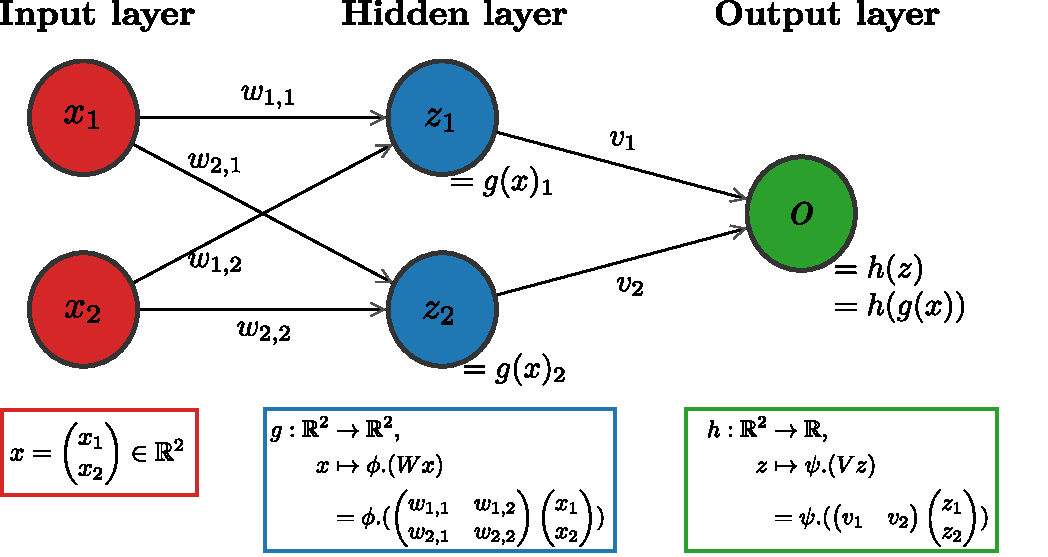
\includegraphics[width=\linewidth]{simple_fnn_example.pdf}
	\caption{Simple FNN example.}
	\label{fig:simple_fnn}
\end{figure}

Figure~\ref{fig:simple_fnn} illustrates the representation of a simple FNN as a directed acyclic graph. Here, the network consists of three layers, an input layer with two nodes, one hidden layer with two nodes and an output layer with one node. The network thus defines a function 
\begin{equation*}
\begin{split}
	f:\R^2 &\to \R, \\
	x&\mapsto f(x) = h(g(x)),
	\end{split}
\end{equation*}
where the functions $g: \R^2 \to \R^2, x \mapsto g(x) = \phi.(Wx)$, $h: \R^2 \to \R, z\mapsto h(z) = \psi.(Vz)$ defining the hidden and output layer, respectively, each consist of a linear transformation with a weight matrix $W\in\R^{2\times 2}$ resp. $V\in\R^2$ followed by a non-linear activation function $\phi:\R\to\R$ resp. $\psi:\R\to\R$. 

\subsection{Neural networks as universal function approximators}\label{sec:nns_universal_approximators}

Generally, FNNs are applied to approximate functions, that, e.g., map some input data $x$ to a label $y$ and thus serve as a classifier. Prior to their successful application in many areas such as pattern and sequence recognition, medical diagnosis, finance or game playing (\cite[pp.~22-26]{Goodfellow2016}), the basic theoretical property of feedforward neural networks as universal function approximators has been investigated and proved in several versions. 

The \textbf{universal approximation theorem} states that a feed-forward neural network with a single layer in addition to the input layer containing a finite number of nodes can approximate any Borel measurable function on a compact subset of a finite-dimensional $\R$-vector space under certain assumptions on the activation function (\cite[pp.~194f.]{Goodfellow2016}). Simple FNNs can thus in theory represent a wide variety of interesting functions when given appropriate parameters; however, the theorem does not say anything about whether those parameters can be actually found by an explicit algorithm. 

One of the first versions of the theorem was formulated and proved by George Cybenko in 1989 (\cite{Cybenko1989} and is presented following \cite[pp.~305-307]{Cybenko1989}.

\begin{definition}
	A function $\sigma: \R \to \R$ is called \textbf{sigmoidal}, if 
	\begin{equation*}
		\sigma(x) \to \begin{cases}
		1 & \text{as} \quad x\to +\infty \\
		0 & \text{as} \quad x\to -\infty.
		\end{cases}
	\end{equation*}
\end{definition}

\begin{theorem}[Universal approximation theorem]\label{universal_approx_thm}
	Let $\sigma$ be a continuous sigmoidal function, let $I_n = [0,1]^n \subset \R^n$ 
	denote the $n$-dimensional unit cube in $\R^n$. Then, functions $G: I_n \to \R$ consisting of finite sums of the form 
	\begin{equation}\label{form-of-G}
	\begin{split}
 		G(x) = \sum_{i=1}^{N} v_i \sigma(w_i^{\top}x + b_i),
	\end{split}
 	\end{equation}
	where $x\in I_n, v_i, b_i \in \R, w_i \in \R^n$ for all $i=1,\dots, N$ are dense in $\mathcal{C}(I_n)$ with respect to the supremum norm, i.e., for any continuous function $f\in \mathcal{C}(I_n)$ and any $\varepsilon >0$, there exist constants $v_i, b_i \in \R$ and vectors $w_i \in \R^n$ for all $i=1,\dots, N$, such that for $G(x)$ as in (\ref{form-of-G})
	\begin{equation*}
	\begin{split}
		\mid G(x) - f(x) \mid < \varepsilon \quad \text{for all } x\in I_n. 
	\end{split}
	\end{equation*}
\end{theorem}

The proof is given for a slightly different scenario of a \textbf{discriminatory} function $\sigma$ and is based on an application of the Hahn-Banach theorem and the Riesz representation theorem. The fact that the Hahn-Banach theorem essentially follows from the axiom of choice already hints at the nature of the universal approximation theorem as a theoretical result without a constructive proof that does not provide us with any practical instruction of how to actually construct these approximating networks for a given function. 

To prove the theorem, we first need to define discriminatory functions: 
\begin{definition}
	A function $\sigma: \R \to \R$ is called \textbf{discriminatory}, if for a measure $\mu$ on $I_n$, it follows from
	$$
	\int_{I_n} \sigma(v^{\top}x + b) d\mu(x) = 0 \quad \text{ for all } v\in\R^n, b \in \R
	$$
	that $\mu \equiv 0$.
\end{definition}

With that definition, we can reformulate the universal approximation theorem as follows:

\begin{theorem}\label{UAT-reformulated}
	Let $\sigma$ be a continuous discriminatory function. Then, finite sums of the form
	\begin{equation}\label{form-of-G-2}
	\begin{split}
		G(x) = \sum_{i=1}^{N} v_i \sigma(w_i^{\top}x + b_i), 
	\end{split}
	\end{equation}
	where $x\in I_n, v_i, b_i \in \R, w_i \in \R^n$ for all $i=1,\dots, N$ are dense in $\mathcal{C}(I_n)$ with respect to the supremum norm. 
\end{theorem}
\begin{proof}
	The following proof is a slightly more detailed version of the proof in \cite[p.~306]{Cybenko1989}.
	Let $\mathcal{G} \subset \mathcal{C}(I_n)$ be the set of functions of the form $G(x)$ as in (\ref{form-of-G-2}). It is clear that $\mathcal{G}$ is a linear subspace of $\mathcal{C}(I_n)$. We prove by contradiction that the closure of $\mathcal{G}$ with respect to the supremum norm is all of $\mathcal{C}(I_n)$. 
	
	Assume for contradiction that the closure $\bar{\mathcal{G}}$ is a proper subspace of $\mathcal{C}(I_n)$. The space $\mathcal{C}(I_n)$ is complete with respect to the supremum norm. Then, it follows from the Hahn-Banach theorem that there is a bounded linear functional $L$ on $\mathcal{C}(I_n)$ with the property that $L\neq 0$ but $L$ vanishes on $\bar{\mathcal{G}}$ and thus also on $\mathcal{G}$. 
	
	$\mathcal{C}(I_n)$ is a Hilbert space with respect to the $L^2$ inner product. Thus, by the Riesz representation theorem, there is a function $l\in \mathcal{C}(I_n)$ such that 
	$$
	L(f) = \langle l,f\rangle_{L^2} = \int_{I_n} f(x)l(x) d\lambda(x) 
	$$ 
	for all functions $f\in\mathcal{C}(I_n)$, where $\lambda$ denotes the Lebesgue measure. 
	
	Then, the function 
	$$
	\mu: \mathcal{B}(I_n) \to \R, \mu(A) := \int_A l(x) d\lambda(x)
	$$
	defines a measure $\mu$ on $I_n$ and $L$ can be written as 
	\begin{equation}\label{form-of-L}
			L(f) = \int_{I_n} f(x) d\mu(x)		
	\end{equation}
	for all $f\in\mathcal{C}(I_n)$. In particular, since obviously $\sigma(v^{\top}(\cdot) + b) \in \bar{\mathcal{G}}$ for all $v \in \R^n, b\in \R$, it follows that
	$$
	L(\sigma(v^{\top}(\cdot) + b)) = \int_{I_n} \sigma(v^{\top}x + b) d\mu(x) = 0
	$$
	for all $v \in \R^n$ and $b\in \R$.
	Since $\sigma$ was assumed to be discriminatory, it follows that $\mu\equiv 0$. We can see from (\ref{form-of-L}) that this implies $L = 0$ on all $\mathcal{C}(I_n)$, contradicting our assumption. Hence, the subspace $\mathcal{G}$ must be dense in $\mathcal{C}(I_n)$.
\end{proof}

The universal approximation theorem, Theorem~\ref{universal_approx_thm}, now follows from Theorem~\ref{UAT-reformulated} and the following lemma: 

\begin{lemma}
	Any bounded, measurable sigmoidal function is discriminatory. In particular, any continuous sigmoidal function is discriminatory.
\end{lemma}
\begin{proof}
	The (rather technical) proof can be found in \cite[pp.~307f.]{Cybenko1989}. 
\end{proof}

It was later shown by Leshno et al. (\cite{Leshno1993}) that FNNs satisfying the assumptions of the universal approximation theorem (Theorem~\ref{universal_approx_thm}) are a universal approximator if and only if the activation function is not polynomial.

In order for FNNs with a single hidden layer to be universal approximators, their layer width can be exponentially large with respect to the desired accuracy. In 2017, Lu et al. (\cite{Lu2017}) proved a universal approximation theorem for deep FNNs with bounded width. In particular, they showed that any Lebesgue integrable function on an $n$-dimensional input space can be approximated with respect to $\mathrm{L}^1$ distance by an FNN of width $n+4$ with ReLU activation functions, if the network depth is allowed to grow.

\subsection{Training neural networks with backpropagation}\label{sec:backprop}
The process of finding a parameter set, i.e., determining weights and biases such that a FNN approximates a specific input-output-mapping is called \textbf{learning} or \textbf{training} of the FNN. The term \textbf{deep learning} thus refers to the process of approximating certain input-output-mappings with deep neural networks. 

More precisely, this is realised by specifying an objective in terms of a \textbf{cost function} that, for example, often denotes a measure of distance between each output value of the FNN and the corresponding training target. If a FNN and the objective are designed such that the cost function is differentiable with respect to the network parameters, we can optimise it by taking its gradient with respect to the parameters and set it to zero, thus "learning" parameters that best approximate the desired mapping, as quantified by the defined objective. 

In this light, nearly all deep learning algorithms can be described as examples of a standard procedure from classical statistical learning: 
Given a dataset, we define a model, a cost function and an optimisation procedure, and aim to optimise the model parameters with respect to the objective specified via the cost function.

If a model includes nonlinearities, such as non-linear activation functions of FNNs, most standard cost functions can no longer be optimised in closed form (\cite[Chapter 5, p.~151]{Goodfellow2016}). This requires an iterative numerical optimisation procedure, such as the gradient descent algorithm, to approximately minimise the cost function. 
Specifically, FNNs are typically trained with the \textbf{backpropagation} algorithm, first developed in \cite{Rumelhart1986} and described by the original authors as follows: "The procedure repeatedly adjusts the weights of the connections in the network so as to minimize a measure of the difference between the actual output vector of the net and the desired output vector." (\cite[p.~533]{Rumelhart1986})
Backpropagation is employed to learn parameters of a neural network such that an arbitrary cost function of the FNN output that is differentiable with respect to the parameters is minimised. 

In the forward pass of one iteration, an input value is passed through all the layers one by one, by applying the function defining the layer with the current set of parameters. 
Having applied all layer functions, the loss for the obtained output value can be calculated.
If we are interested in learning a classifier, i.e., a mapping assigning labels to each input, we also regard the loss as a function of the true label to compare the output to.
Since the output has been derived from applying the FNN function to the input and that function depends on the current parameter values, we can also for a fixed input regard the loss as a function of the network parameters. Assuming it is differentiable with respect to the parameters, we can calculate the partial derivatives of the loss function with respect to each parameter and set the derivatives to zero. 
Due to the structure of the FNN as a function composition, the chain rule has to be applied multiple times to obtain the gradients: The loss directly depends on the parameters of the last layer, which depend on those of the second last layer, etc. In that way, the gradients are propagated backwards through the network to obtain the partial derivative with respect to each parameter -- hence the term backpropagation. After obtaining the partial derivatives with respect to all the parameters, the current parameter values can be updated according to the gradient descent algorithm. Proceeding in this way, the cost function is iteratively optimised with respect to the network parameters and the network is thereby trained to ultimately approximate the desired input-output mapping. Neccessary conditions for this procedure are a scalar loss value for each input and a differentiable FNN structure.

\begin{figure}
	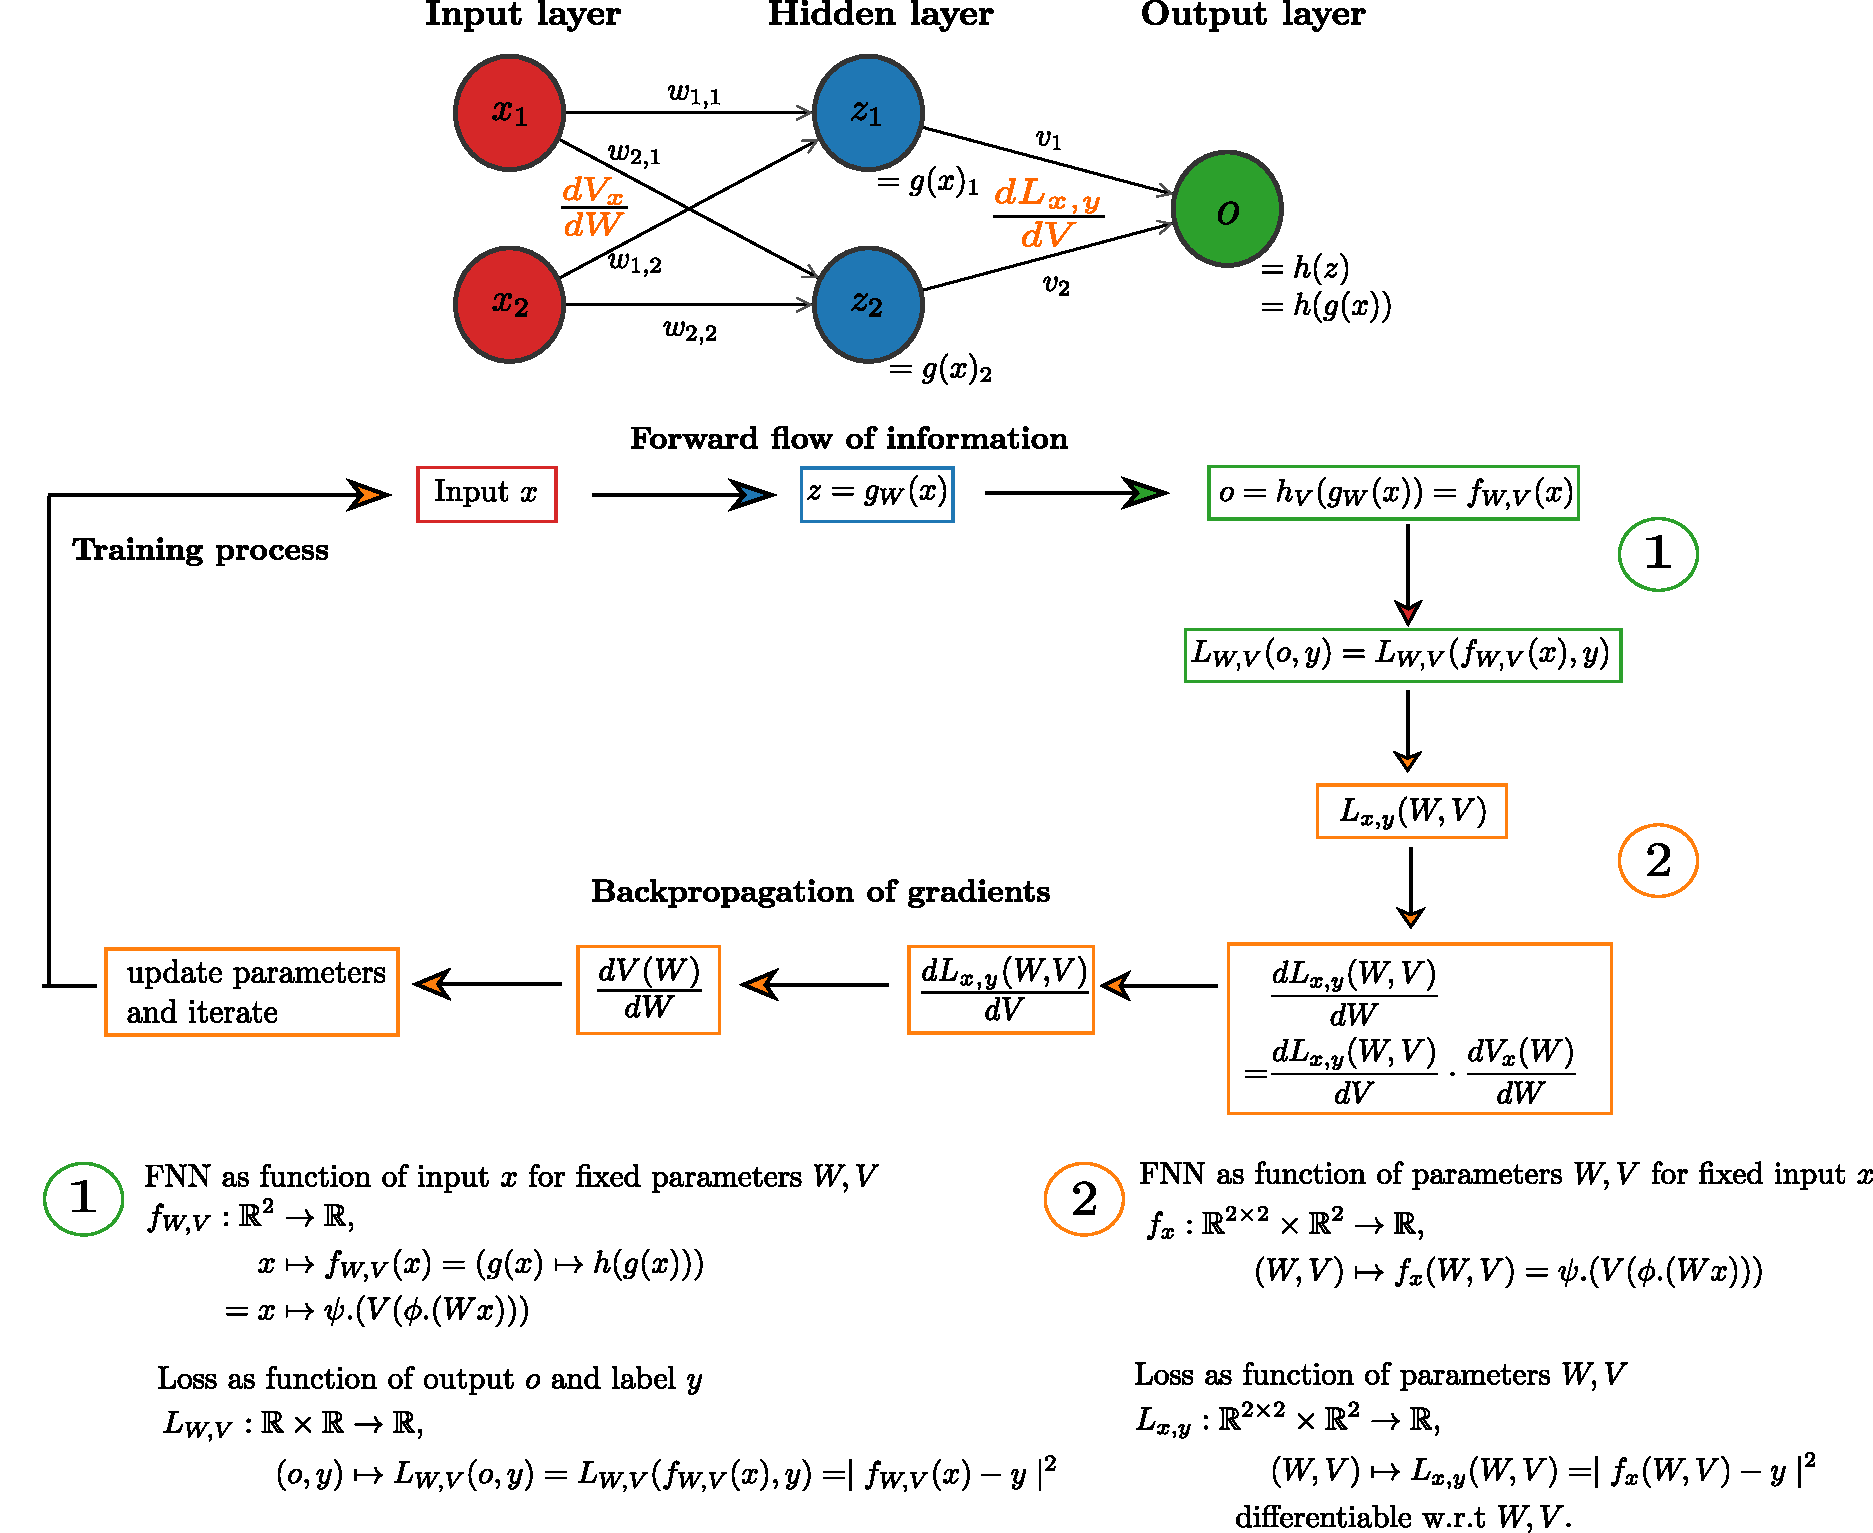
\includegraphics[width=1.1\linewidth]{simple_fnn_backprop.pdf}
	\caption{Training an FNN with backpropagation.}
	\label{fig:backprop}
\end{figure}

Figure~\ref{fig:backprop} illustrates the backpropagation algorithm with the simple FNN example from Figure~\ref{fig:simple_fnn}. The loss function is chosen to be the squared difference between an FNN output and the corresponding true label.

Often the \textbf{stochastic gradient descent (SGD)} algorithm is employed for training, which uses randomly drawn minibatches of data $\mathcal{M} \subset \mathcal{D}$ to obtain an unbiased estimate $\hat{L}(\theta, \varepsilon)$ of the objective $L(\theta)$, i.e., $\E_{\P^{\mathcal{E}}}[\hat{L}(\theta, \cdot)] = L(\theta)$ for FNN parameters $\theta$, where the random variable $\mathcal{E}$ describes the sampling of the minibatch (\cite[p.~72]{Kingma2019}). In the $k$-th step of the SGD algorithm, the current parameter value $\theta_k$ is updated to $\theta_{k+1}$ according to
$$
	\theta_{k+1} \leftarrow \theta_k + \alpha_k \cdot \nabla_{\theta} \hat{L}(\theta, \varepsilon_k),
$$
where $\alpha_k$ denotes the stepsize and is also called the \textbf{learning rate} and $\varepsilon_k$ represents a realisation of $\mathcal{E}$ corresponding to the sampling of the current minibatch. 
Training a FNN can now be achieved by repeating this updating step which is also called a training \textbf{epoch} until a pre-defined convergence criterion of the loss function is reached. 
From now on, all FNNs are assumed to be differentiable with respect to the parameters, thus allowing for an iterative optimisation using (stochastic) gradient descent.

\subsection{Generative models}\label{sec:generative_model_examples}

Neural networks can be trained to approximate different types of input-output relations and have been successfully applied in various classification tasks.
Having learned a classifier and thus being able to discriminate and label new observations does not, however, yield any insight into the data-generating process itself. Additionally, this form of supervised learning typically requires large amounts of labelled training data. After training, the deterministic function represented by such a discriminative neural network will always produce the exact same label for a specific observation and thus does not provide any information about uncertainty on the label assignment (\cite[pp.~2f.]{Kingma2019}). 

To understand the data-generating mechanisms and characterise their variability as a result of random forces governing the process, a \textbf{generative} deep learning model (as opposed to a discriminative one) aims at modelling a joint probability distribution over all the variables (\cite[Chapter~20, p.~651]{Goodfellow2016}). It thus simulates how the data is generated in the real world and accounts for the stochastic nature of that process. A further advantage is that a generative deep learning model can directly learn from data in an unsupervised manner and does not require labelled training examples. 

Having successfully trained a generative model in the form of a neural network then means having captured the process underlying these original observations and formulated it as a probability distribution. As a direct consequence, the model can generate new samples that exhibit the central patterns and structure of the original data. This artificial data can be useful for, e.g., sample size calculations for the planning of future experiments or for settings where due to data protection rules to guarantee privacy it is not possible to share individual-level data.   

While all generative deep learning models share the characteristic of representing a multivariate probability distribution, they differ in the way that distribution is specified. 
In the following, three commonly used examples of deep generative models are briefly reviewed. 

\textbf{Restricted} and \textbf{deep Boltzmann machines (RBMs/DBMs)} are energy-based models, i.e., they define the joint probability distribution of a multi-dimensional binary random vector using an energy function. Originally, they were introduced as a general approach to learning arbitrary probability distributions over binary vectors (\cite{Salakhutdinov09}). The probability distribution is parameterised by a neural network with one (in RBMs) or more (in DBMs) hidden layers. To approximate it, a partition function has to be learned that is generally computationally intractable. However, the specific structure of the neural network allows for efficient Markov Chain Monte Carlo (MCMC) approximation of the desired distributions by using Gibbs Sampling (\cite[Chapter~20, pp.~651-662]{Goodfellow2016}).

Training \textbf{generative adversarial networks (GANs)} (\cite{Goodfellow2014}) can be described as a two-player minimax game of a generator and a discriminator that are both specified by neural networks: Given a dataset and a pre-defined distribution of an input noise random variable, the generative network represents a mapping from the initial distribution to the data distribution the GAN aims to model. The discriminator, a second neural network, outputs the probability that a given input came from the true data distribution rather than from the output distribution of the generator. The discriminator is then trained to maximise the probability of correctly distinguishing between samples from the two, while the generator is simultaneously trained to increase the error rate of the discriminator's classification, i.e., to fool the discriminator. 
The probability distribution function of the original data is thus only available implictly through the samples produced by the generative network.

Finally, a \textbf{variational autoencoder (VAE)}(\cite{Kingma2013}) aims at learning a low-\\
dimensional representation of the input data given by a latent random variable. The transformations from the original data space to the latent space and back are given by independently parameterised, but jointly optimised neural networks: The encoder learns a transformation from the input data to the typically lower-dimensional latent space. It outputs the parameters of an approximation to the posterior distribution of the latent variable given the input data. The generative network is trained to learn the conditional distribution of the input data given a sample of the posterior distribution of the latent variables from the encoder network, such that it approximates the true underlying data distribution. Thus, the encoder is the approximate inverse of the generative model and the two networks are trained jointly, such that the encoder learns a meaningful representation of the input data that can in turn be successfully decoded to samples from the data distribution by the generative network. 

In comparison to GANs, VAEs are reported to have complimentary properties (\cite[p.~5]{Kingma2019}): While GANS can generate subjectively realistic samples, they often only cover a part of the true data distribution, whereas VAEs tend to generate "blurrier", more dispersed samples, but better capture the underlying density. 

Further advantages of the VAE are that it explicitly parameterises the probability distributions involved and that it learns to compress the data into a low-dimensional representation that reflects the central factors of variation governing the dataset. These properties allow us to integrate smoothness constraints and explicit modelling of temporal dynamics into the model and learn a more structured, interpretable low-dimensional representation that provides insight into the main underlying trends driving the temporal patterns in the original data. For these reasons, my own model is based on the framework of a variational autoencoder. In the following sections,I outline the theoretical foundation on which the VAE is build and explain the model architecture and training procedure in detail.  

\section{Variational inference}\label{sec:VI}

\subsection{Prerequisites and notation}\label{sec:inference_basics_notation}
The mathematical framework for the following sections is as follows: 
Let $\Omega := \R^p$, $\mathcal{F} := \mathcal{B}(\R^p)$ and $(\Omega, \mathcal{F}, (\P_{\theta})_{\theta\in \Theta})$ be a parametric statistical model with parameter space $\Theta\subset \R^d$ for some $d\in \N$. Let $\P$ be a probability measure on $(\Omega, \mathcal{F})$, let $X$ be a real-valued $p$-dimensional random variable on $(\Omega, \mathcal{F}, \P)$ with probability distribution $\P^X$, let $\mathcal{D} = \lbrace x_1, \dots, x_n \rbrace $ be a dataset of $n$ independent samples of $X$. We assume that the true distribution $\P^X$ is unknown and attempt to approximate it with a member of the family $(\P_{\theta})_{\theta\in\Theta}$.
Let $Z$ be a second lower-dimensional real-valued variable on $(\Omega, \mathcal{F}, \P)$ with probability distribution $\P^Z$ which we do not observe but assume to govern the underlying mechanism according to which observations of $X$ are generated (see Section~\ref{sec:bayesian_inference}). We assume our parametric family to be flexible enough to include or approximate the true distributions of $X$ and $Z$ and their joint distribution.

Additionally, we assume that for every $\theta \in \Theta$, $\P_{\theta}$ is absolutely continuous with respect to the Lebesgue measure $\lambda$. Then, it follows from the Radon-Nikodym theorem that for every $\theta \in \Theta$, $\P_{\theta}$ admits a density with respect to $\lambda$ that we denote by $p_{\theta} = \frac{dP_{\theta}}{d\lambda}$. We assume the Lebesgue measure to be an equivalent measure for all probability measures $\P_{\theta}$, $\theta\in \Theta$, implying that all densities with respect to the Lebesgue measure are strictly positive. 

In general, I denote random variables with capital letters and their realisations with small letters. To denote densities of random variables (provided they exist), I use small letters with the random variable as a subscript, i.e., $p_Z(\cdot)$ is the density of $Z$. For ease of notation, I abbreviate conditional distributions and densities by writing, e.g., $p_{X\mid z}(x)$ for $p_{X\mid Z=z}(x)$. I write $\E_p[q]$ for the integral $\int_{-\infty}^{\infty}q(x)\cdot p(x)~dx$, where $q$ and $p$ are densities with respect to the Lebesgue measure $\lambda$, such that $\E_p[q] = \E[q(X)]$ for a random variable $X$ on $(\Omega, \mathcal{F}, \P)$ with $\frac{d\P^X}{d\lambda} = p$, and therefore $\E[q(X)] = \int_{\Omega} q(X)~d\P = \int_{-\infty}^{\infty} q(x)\cdot p(x)~dx$.

I denote with $p_X(x,\theta)$ the likelihood function that parameterises the family of potential densities of $X$ as a function of the parameter $\theta$, i.e., evaluates the likelihood of a particular realisation $x$ of $X$ under the density defined by a specific $\theta$. Analoguously, I denote with $p_{X,Z}: \R^2 \times \Theta, (x,z,\theta) \mapsto p_{X,Z}(x,z,\theta)$ for realisations $x$ and $z$ of $X$ and $Z$, respectively, the function parameterising the potential joint densities of $X$ and $Z$ as a function of $\theta$ and also use this notation to parameterise families of potential densities of a single random variable or of conditional probability distributions. For simplicity, I refer to these potential "candidate" densities of distributions or random variables simply as densities.

\subsection{Bayesian inference}\label{sec:bayesian_inference}

The data are assumed to be generated in a two-step process (\cite[p.~2]{Kingma2013}): First, a sample $z$ of a the lower-dimensional random variable $Z$ on $(\Omega, \mathcal{F},\P)$ is drawn according to its distribution $z \sim \P^Z$, called the \textbf{prior distribution}. We assume that $\P^Z = \P_{\theta^{Z}}$ for a $\theta^{Z} \in \Theta$. Secondly, a sample $x = x_{i}$ for some $i\in \lbrace 1,\dots, n\rbrace$ is drawn from the conditional distribution $\P_{X\mid z}$. We assume the joint distribution $\P^{X,Z}$ to also be a member of the family $(\P_{\theta})_{\theta\in\Theta}$, such that the density of the conditional distribution of $(X\vert z)$ for a realisation $z$ of $Z$, given by the expression
$$
p_{X\mid z}(x) :=  \frac{p_{X,Z}(x,z)}{p_{Z}(z)},
$$
can also be parameterised by $\Theta$. We assume that the parameters $\theta^Z$ and $\theta^{(X,Z)}$ characterising the true distribution of $Z$ and the true joint distribution of $X$ and $Z$ are unknown. 

Intuitively, this scenario implies that the variation in our data is based on a few unobserved factors of variation corresponding to the dimensions of the latent random variable $Z$ that we would like to recover along with the details of how the data are generated from the low-dimensional representation $Z$. To achieve that, since only $X$ but not $Z$ is observed, we have to reverse the process and use the observations of $X$ to enrich our knowledge of $Z$, i.e., we condition the distribution of $Z$ on the observations of $X$ and compute the density of the \textbf{posterior distribution} of $Z$ in Bayesian terminology (see \cite[pp.~57-63]{Czado2011}, \cite[p.~70]{Kingma2019} for more on Bayesian inference). According to Bayes' rule, we obtain
\begin{equation}\label{bayes_with_z-posterior}
p_{Z\mid x}(z) = \frac{p_{X,Z}(x, z)}{p_{X}(x)} = \frac{p_{X,Z}(x, z)}{\int p_{X,Z}(x, z) dz}.
\end{equation}

In the last expression of (\ref{bayes_with_z-posterior}), the marginal data likelihood is rewritten as an integral of the joint density of $X$ and $Z$ over all values of $Z$. A model that parameterises such a family of potential joint distributions of the observed and latent variables with FNNs is called a \textbf{deep latent variable model (DLVM)} as in \cite[pp.~12f.]{Kingma2019}. 
Training a DLVM that parameterises $p_{X,Z}$ as a function of $\theta$ means to find the parameters $\theta_{X,Z}$ such that $p_{X,Z}(\cdot, \theta_{X,Z})$ equals the true density of $\P^{X,Z}$.  
In such a DLVM, for a fixed $\theta$ the marginal likelihood of a sample $x$ of $X$ is given by
\begin{equation}\label{marginal-likelihood}
	p_X(x,\theta) = \int_{-\infty}^{\infty} p_{X,Z}(x,z,\theta)dz,	
\end{equation}
which shows that an advantage of these models is their expressivity while maintaining a simple structure: even for relatively simple factors $p_{X,Z}(x,z,\theta)$, the marginal density $p_{X}$ can be very complex and DLVMs can thus effectively model complicated underlying distributions $\P^X$(\cite[pp.~12f.]{Kingma2019}). 

To obtain a maximum likelihood estimate for $\theta$ in DLVMs modelling joint distributions of input data and latent variables, the data likelihood $p_{X}(x,\theta)$ has to be maximised with respect to $\theta$. 
From (\ref{marginal-likelihood}), we see that calculating this marginal likelihood from the joint distribution involves integrating over all possible configurations $(x,z)$. Even for moderately complex models, such as DLVMs with a non-linear hidden layer, this is computationally intractable, implying the intractability of the posterior (\cite[p.~13]{Kingma2019}).

If, however, the density of the conditional distribution $p_{Z\mid x}(\cdot,\theta)$ is tractable to compute, the \textbf{expectation maximisation (EM)} algorithm (\cite{Rubin1977}) can be used to approximate the maximum likelihood estimate of the marginal likelihood, which consists of iteratively applying the following two steps until convergence:

1. \textbf{Expectation step:} Define $q(\theta\mid \theta^{(k)})$ as the expected value of the log likelihood function of the joint distribution of $X$ and $Z$ with respect to the conditional distribution of $Z$ given a sample $x$ of $X$ under the current estimate of $\theta^{(k)}$:
$$
	q(\theta\mid \theta^{(k)}) := \E_{p_{Z\mid x}(\cdot, \theta^{(k)})}\left[\log\left(p_{X,Z}(x, \cdot, \theta)\right)\right].
$$

2. \textbf{Maximisation step:} Find the parameter $\theta^{(k+1)}$ that maximises this quantity:
$$
	\theta^{(k+1)} := \arg \max_{\theta} q\left(\theta\mid \theta^{(k)}\right).
$$

\subsection{Inference as an optimisation problem}\label{sec:inference_as_optimisation}

In DLVMs, the marginal likelihood $p_{X}$ of the data-generating random variable $X$ is typically intractable. But since they are defined as a model parameterising the joint density $p_{X,Z}(x,z,\theta)$, this joint distribution is tractable to compute in DLVMS. Hence, we can see from (\ref{bayes_with_z-posterior}) that the posterior $p_{Z\mid x}(z, \theta)$ is tractable if and only if the marginal likelihood is tractable (\cite[p.~14]{Kingma2019}). 

More broadly, this problem applies to any sufficiently complex Bayesian model including latent variables, since inference in a Bayesian model always amounts to conditioning on data and computing the posterior. If this is not computationally tractable, approximative inference is required (\cite[p.~2]{Blei}). A classical approach for that is Markov chain Monte Carlo (MCMC) sampling, which amounts to constructing a Markov chain on $Z$ such that its stationary distribution is that of the posterior $\P_{\theta}^{Z\mid x}$, sampling from the chain and approximating the posterior with an empirical estimate constructed from the samples (\cite[p.~2]{Blei}). MCMC sampling is a common and widely used tool to perform approximate inference in Bayesian statistics that has been extensively studied (for an overview see, e.g., \cite{Casella2004}). 

\textbf{Variational inference} (\cite{Blei}) represents an alternative strategy to approximate intractable posterior distributions. The key idea is to reframe the problem of performing approximate inference as an optimisation problem rather than using sampling. To this end, we define a family $\mathcal{Q}$ of approximate densities over the latent variables $Z$ and aim to find the member of the family that minimises a measure of distance $d(\cdot,\cdot)$ to the exact posterior density:
\begin{equation}\label{var_inference_generaldistance}
	q^*_{Z\mid x} = \arg \min_{q_{Z\mid x}\in\mathcal{Q}} d(q_{Z\mid x},p_{Z\mid x}).
\end{equation}

Variational inference in general has advantages over MCMC in settings where a faster approximation of a posterior is desired than can be achieved with MCMC algorithms, such as for large datasets or very complex models. For a more detailed discussion of the strength and weaknesses of the two approaches and typical scenarios in which to use either, see \cite[p.~3]{Blei} and the references mentioned there.

\subsection{The Kullback-Leibler divergence}\label{sec:KL-div}

As a measure of distance between probability distributions, the \textbf{Kullback-Leibler (KL) divergence} (\cite[p.~72]{Goodfellow2016}) is used:
\begin{definition}
	Let $(\Omega,\mathcal{F})$ be a measurable space and let $\P$, $\Q$ be probability measures on $(\Omega, \mathcal{F})$ such that $\P$ is absolutely continuous with respect to $\Q$, i.e., admits a density with respect to $\Q$ denoted by $\frac{d\P}{d\Q}$. The \textbf{Kullback-Leibler (KL) divergence} from $\Q$ to $\P$ is defined as
	$$\dkl(\P\Vert \Q) = \int_{\Omega} \log\left(\frac{d\P}{d\Q}\right) d\P.
	$$   
	If $\P$ and $\Q$ are absolutely continuous with respect to the Lebesgue measure $\lambda$, denoting the densities $p=\frac{d\P}{d\lambda}$ and $q=\frac{d\Q}{d\lambda}$, the Kullback-Leibler divergence can be rewritten as an expectation with respect to $P$: 
	$$
	\dkl(\P\Vert \Q) = \E\left[\log\left(\frac{d\P}{d\Q}\right) \right] = \int_{\Omega} \log\left(\frac{d\P}{d\Q}\right) d\P = \int_{-\infty}^{\infty} \log\left(\frac{p}{q}\right) p~d\lambda = \E_{p}\left[\log\left(\frac{p}{q}\right)\right].
	$$
	In this case, I equivalently write $\dkl(p\Vert q)$ for $\dkl(\P\Vert \Q)$.
\end{definition}

\begin{rmk}\label{rmk:kl-div-nonnegative}
	It follows from Jensen's inequality that the Kullback-Leibler divergence is always non-negative:
	\begin{equation*}
	\begin{split}
		\dkl(\P\Vert \Q)  &= \int_{\Omega} \log\left(\frac{d\P}{d\Q}\right) d\P = \int_{\Omega} -\log\left(\frac{d\Q}{d\P}\right) d\P \\
		& \geq -\log \left(\int_{\Omega} \frac{d\Q}{d\P} d\P\right) = -\log \left(\int_{\Omega} d\Q\right) = -\log(1) = 0,
	\end{split}
	\end{equation*}
	where the $\geq$ results from applying Jensen's inequality. 
	
	The KL divergence is equal to $0$ if and only if the two probability measures $\P$ and $\Q$ are equal.
	However, the KL-divergence is not symmetric and hence is not a metric.
	Nonetheless, it is widely used as a notion of distance between two probability distributions in machine learning and statistics. 
\end{rmk}

Quantifying the difference between members of the variational family $\mathcal{Q}$ and the exact posterior with the KL-divergence, our optimisation problem (\ref{var_inference_generaldistance}) becomes
\begin{equation}\label{var_inference_withkl}
	q^*_{Z\mid x} = \arg \min_{q_{Z\mid x}\in\mathcal{Q}} \dkl(q_{Z\mid x}\Vert p_{Z\mid x}).
\end{equation}
The complexity of this optimisation depends on the complexity of the family $\mathcal{Q}$ of candidate approximate densities. While a simpler structure of $\mathcal{Q}$ allows for a simpler and more efficient optimisation, a larger, more flexible family $\mathcal{Q}$ can potentially capture a density closer to the exact posterior. 

\subsection{Calculus of variation}\label{sec:calculus_of_variation}
The term "variational inference" refers to the theory of calculus of variation, a branch of functional analysis, which centers on the fundamental idea of minimising a functional on some (typically infinite-dimensional) function space. A classical example is given by the Dirichlet energy functional
$$
	E: \mathcal{H}^1(U) \to \R, \quad u\mapsto \frac{1}{2}\int_U \Vert \nabla u(x)\Vert^2 dx,
$$
where $U\subset \R^n$ is an open subset and $\mathcal{H}^1(U)$ denotes the Sobolev space on $U$. The functions that minimise the Dirichlet energy and satisfy certain boundary conditions are exactly the solutions of the partial differential equation given by Laplace's equation $-\Delta u(x) = 0$ for all $x\in U$ subject to appropriate boundary conditions.  More generally, many problems in the scope of calculus of variation have applications in the field of partial differential equations. 

In variational inference, the functional to be minimised is given by the distance measure between the probability distributions, often the KL-divergence, while the space of functions over which it is minimised is given by the variational family $\mathcal{Q}$. In my setting, I will exclusively use a parametric family $\mathcal{Q} = (q_{Z}(\cdot,\phi))_{\phi\in\Phi}$ with $\Phi \subset \R^e$ for some $e\in \N$, so that the space of approximate posterior distributions is completely determined by the parameter space $\Phi$ and hence finite-dimensional. Therefore, here the calculus of variation does not have to be employed to solve the approximation problem.

\subsection{The evidence lower bound}\label{sec:ELBO}

The following derivation of the evidence lower bound is based on \cite[pp.~6f.]{Blei} and \cite[pp.~16-18]{Kingma2019}. 

Returning to our optimisation problem of finding $q_{Z\mid x}^*$ as in (\ref{var_inference_withkl}), rearranging the terms of the KL-divergence yields
	\begin{equation}\label{kl-decomposition}
\begin{split}
\dkl(q_{Z\mid x}\Vert p_{Z\mid x})  &= \E_{q_{Z\mid x}}\left[\log\left(\frac{q_{Z\mid x}}{p_{Z\mid x}}\right)\right] \\
&= \E_{q_{Z\mid x}}[\log(q_{Z\mid x})] - \E_{q_{Z\mid x}}[\log(p_{Z\mid x})] \\
&= \E_{q_{Z\mid x}}[\log(q_{Z\mid x})] - \E_{q_{Z\mid x}}\left[\log\left(\frac{p_{X,Z}(x,\cdot)}{p_{X}(x)}\right)\right] \\
&= \E_{q_{Z\mid x}}[\log(q_{Z\mid x})] - \E_{q_{Z\mid x}}[\log(p_{X,Z}(x,\cdot))] + \log(p_{X}(x)),
\end{split}
\end{equation}
where we used the linearity of the expectation and the fact that $\log(p_{X}(x))$ is a constant with respect to $q_{Z\mid x}$. The last line shows that in fact the KL-divergence we aim to minimise depends on $\log(p_{X}(x))$ which we assumed to be intractable. That intractability implies that of the posterior $p_{Z\mid x}$ (as described in Section~\ref{sec:bayesian_inference}) and was our motivation to approximate the posterior with variational inference in the first place. However, the observation that $\log(p_{X}(x))$ is a constant with respect to $q_{Z\mid x}$ also implies that minimising the expression
$\E_{q_{Z\mid x}}[\log(q_{Z\mid x})] - \E_{q_{Z\mid x}}[\log(p_{X,Z}(x,\cdot))]$
is equivalent to minimising $\dkl(q_{Z\mid x}\Vert p_{Z\mid x})$ with respect to $q_{Z\mid x}$, i.e.,
$$
q_{Z\mid x}^* = \arg \min_{q_{Z\mid x}\in\mathcal{Q}} \dkl(q_{Z\mid x}\Vert p_{Z\mid x}) = \arg \min_{q_{Z\mid x}\in\mathcal{Q}} \E_{q_{Z\mid x}}[\log(q_{Z\mid x})] - \E_{q_{Z\mid x}}[\log(p_{X,Z}(x,\cdot))].
$$

Re-organising the terms in the last line of (\ref{kl-decomposition}) and using the non-negativity of the KL-divergence from Remark~\ref{rmk:kl-div-nonnegative}, we obtain
\begin{equation}\label{lowerbound_on_logpx}
\begin{split}
	\log(p_{X}(x)) &= \E_{q_{Z\mid x}}[\log(p_{X,Z}(x, \cdot))] - \E_{q_{Z\mid x}}[\log(q_{Z\mid x})] + \dkl(q_{Z\mid x}\Vert p_{Z\mid x})\\
	&\geq \E_{q_{Z\mid x}}[\log(p_{X,Z}(x, \cdot))] - \E_{q_{Z\mid x}}[\log(q_{Z\mid x})].
\end{split}
\end{equation}
This shows that $\E_{q_{Z\mid x}}[\log(p_{X,Z}(x, \cdot))] - \E_{q_{Z\mid x}}[\log(q_{Z\mid x})]$, the negative of the equivalent objective $\E_{q_{Z\mid x}}[\log(q_{Z\mid x})] - \E_{q_{Z\mid x}}[\log(p_{X,Z}(x, \cdot))]$ defines a lower bound on the marginal data likelihood $\log(p_{X}(x))$. Because the marginal data likelihood is also called the evidence in Bayesian terminology, this expression is called the \textbf{evidence lower bound (ELBO)}
$$
\elbo(x, q_{Z\mid x}) = \E_{q_{Z\mid x}}[\log(p_{X,Z}(x, \cdot))] - \E_{q_{Z\mid x}}[\log(q_{Z\mid x})].
$$
Since minimising the KL divergence with respect to $q$ is equivalent to minimising $\E_{q_{Z\mid x}}[\log(q_{Z\mid x})] - \E_{q_{Z\mid x}}[\log(p_{X,Z}(x, \cdot))]$, which is equivalent to maximising \\
$\E_{q_{Z\mid x}}[\log(p_{X,Z}(x, \cdot))] - \E_{q_{Z\mid x}}[\log(q_{Z\mid x})]$, it follows that minimising the KL-divergence $\dkl(q_{Z\mid x}\Vert p_{Z\mid x})$ is equivalent to maximising the ELBO and 
$$
q_{Z\mid x}^* = \arg \min_{q_{Z\mid x}\in\mathcal{Q}} \dkl(q_{Z\mid x}\Vert p_{Z\mid x}) = \arg \max_{q_{Z\mid x}\in\mathcal{Q}} \elbo(x, q_{Z\mid x}).
$$
From (\ref{lowerbound_on_logpx}) we can see that the KL-divergence $\dkl(q_{Z\mid x}\Vert p_{Z\mid x})$ determines the gap between the ELBO and the marginal data likelihood $\log(p_{X}(x))$ and thus the tightness of the bound. Rewriting the ELBO can give us an intuition about the properties of the optimal variational density (\cite[pp.~6f.]{Blei}):
\begin{equation}\label{elbo_form_recerror_kldivtoprior}
	\begin{split}
		\elbo(x, q_{Z\mid x}) &= \E_{q_{Z\mid x}}[\log(p_{X,Z}(x, \cdot))] - \E_{q_{Z\mid x}}[\log(q_{Z\mid x})] \\
		&= \E_{q_{Z\mid x}}[\log(p_{X\mid Z}(x) p_Z)] - \E_{q_{Z\mid x}}[\log(q_{Z\mid x})] \\
		&= \E_{q_{Z\mid x}}[\log(p_{X\mid Z}(x))] + \E_{q_{Z\mid x}}[\log(p_{Z})] - \E_{q_{Z\mid x}}[\log(q_{Z\mid x})] \\
		&= \E_{q_{Z\mid x}}[\log(p_{X\mid Z}(x))] + \E_{q_{Z\mid x}}\left[\log\left(\frac{p_{Z}}{q_{Z\mid x}}\right)\right] \\
		&= \E_{q_{Z\mid x}}[\log(p_{X\mid Z}(x))] - \dkl(q_{Z\mid x}\Vert p_{Z}).
	\end{split}
\end{equation}
The first term in the last line shows that maximising the ELBO encourages densities placing mass on configurations of latent variables that explain the observed data, while the second term encourages densities that are close to the prior. 

Parameterising the potential candidate prior and posterior densities of $Z$ and $Z\vert x$ for a sample $x\in\mathcal{D}$ with $\theta$ as in Section~\ref{sec:bayesian_inference} and (e.g.) Equation (\ref{bayes_with_z-posterior}), we can define the ELBO as a function of not only the approximate posterior $q_{Z\mid x}$ and the data $x\in\mathcal{D}$, but also of the parameter $\theta$ defining the densities of $Z$ and $Z\vert x$ that is called the \textbf{model parameter}. Additionally, we assume a parametric variational family $\mathcal{Q} = (q_{Z\mid x}(\cdot, \phi))_{\phi \in \Phi}$ with $\Phi \subset \R^e$ for an $e\in \N$, so that the finite-dimensional space $\Phi$ completely characterises the family of approximate posteriors, and call the parameter $\phi \in \Phi$ the \textbf{variational parameter}. 
As a result, we can view the ELBO as a function of the data $x\in \mathcal{D}$, the model parameter $\theta$ and the variational parameter $\phi$ 
\begin{equation}\label{elbo-as-function-of-theta-and-phi}
\begin{split}
	\elbo(x,\theta, \phi) &= \E_{q_{Z\mid x}(\cdot,\phi)}[\log(p_{X,Z}(x, \cdot, \theta))] - \E_{q_{Z\mid x}(\cdot,\phi)}\left[\log\left(q_{Z\mid x}(\cdot, \phi)\right)\right] \\
	&= \E_{q_{Z\mid x}(\cdot,\phi)}[\log(p_{X\mid Z}(x,\theta))] - \dkl(q_{Z\mid x}(\cdot,\phi)\Vert p_{Z}(\cdot,\theta)).
\end{split}
\end{equation}

Note that since the ELBO is a lower bound on $\log(p_{X}(x,\theta))$, maximising the ELBO with respect to $\theta$ yields an approximation to the maximum likelihood estimate for $\theta$. That approximation is better the smaller the KL-divergence 
$$\dkl(q_{Z\mid x}(\cdot,\phi)\Vert p_{Z\mid x}(\cdot,\theta)),$$ 
that determines the tightness of the bound. We can thus obtain both approximate maximum likelihood estimates for $\theta$ and an optimal variational density $q$ if we maximise the ELBO both with respect to $\theta$ and $\phi$. The search of finding optimal parameters $\theta$ is referred to as \textbf{learning} and the process of finding parameters $\phi$ of an optimal approximate posterior $q$ as \textbf{inference} (\cite[p.~15]{Kingma2019}).

\subsection{Variational expectation maximisation}\label{sec:variational_EM}

Maximising the ELBO with respect to both $\theta$ and $\phi$ can be formulated as a variation of the EM-algorithm from Section~\ref{sec:bayesian_inference} called the \textbf{variational expectation maximisation} algorithm and can also be viewed as coordinate ascent on the ELBO (\cite[p.~71]{Kingma2019}, \cite{NealHinton1998}). It assumes a parametric variational familiy $\mathcal{Q} = (q_{\phi}(z))_{\phi\in\Phi}$ with $\Phi \subset \R^e$ for some $e\in \N$ and estimates \textbf{local} variational parameters $\phi_i$ for each individual sample $x_i$.

As for classical EM, the algorithm starts with (random) initial values of $\theta^{(0)}$ and $\phi_{i=1,\dots, n}^{(0)}$ and iteratively applies the following steps: 

1. \textbf{Expectation step:} For all $i=1,\dots, n$, maximise the ELBO with respect to $\phi_i$ and define
\begin{equation}\label{e-step_variationalEM}
\phi_i^{(k+1)} := \arg \max_{\phi} \elbo(x_i,\theta^{(k)}, \phi_i).
\end{equation}

2. \textbf{Maximisation step:} Maximise the ELBO with respect to $\theta$ and define
\begin{equation}
\theta^{(k+1)} := \arg \max_{\theta} \sum_{i=1}^n \elbo(x_i,\theta, \phi_i^{(k+1)}).
\end{equation}

Note that, as shown before, the objective in (\ref{e-step_variationalEM}) is equivalent to finding $\arg \min_{\phi} \dkl(q_{Z\mid x}(\cdot,\phi) \Vert p_{Z\mid x}(\cdot,\theta^{(k)}))$.

\section{Variational autoencoder}\label{sec:VAE}

The variational autoencoder, briefly described in Section~\ref{sec:generative_model_examples}, is a framework to efficiently perform approximate inference and learning. In short, it is a generative deep learning model consisting of two coupled, jointly optimised neural networks that parameterise an approximate posterior of a latent random variable given observations and the conditional distribution of the data given a sample from the posterior over the latent variables. The training objective is given by the ELBO (\ref{elbo-as-function-of-theta-and-phi}) that is optimised with respect to both the model parameters and the variational parameters using SGD. The following presentation is based on the paper first proposing VAEs \cite{Kingma2013} and \cite[pp.~15-27]{Kingma2019}.

\subsection{Model overview}\label{sec:VAE_model_overview}
The VAE proposes a solution to the three related problems in the setting of intractabilities of the marginal likelihood 
$$p_X(\cdot,\theta) = \int p_{X,Z}(\cdot,z,\theta)dz$$ 
and/or the posterior density
$p_{Z\mid x}(\cdot,\theta)$
for a potentially large dataset where sampling-based MCMC methods would be too slow, namely efficient approximation of maximum likelihood estimates for the parameters $\theta^Z, \theta^{(X,Z)}$, efficient approximate posterior inference of $Z\vert X$ and efficient approximate marginal inference of the underlying variable $X$ (\cite[pp.~2f.]{Kingma2013}). 
Since the latent variable $Z$ encodes a low-dimensional representation of data, the VAE can be seen as a method for inferring these ideally semantically meaningful, statistically independent factors of variation in data. This process is generally known as unsupervised representation learning, and VAEs have been extensively employed for that purpose (\cite[p.~4]{Kingma2019}).

To handle the intractabilities of the marginal likelihood and posterior, a parametric family of distributions $\mathcal{Q}= (q_{Z\mid x}(\cdot, \phi))_{\phi\in\Phi}$ with $\Phi\subset \R^e$ for some $e\in \N$ is introduced. We then aim to optimise the variational parameters $\phi$ to find a family member $q_{Z\mid x}(\cdot, \phi)$ that approximates the true posterior as in Section~\ref{sec:VI}, such that $q_{Z\mid x}(z, \phi) \approx p_{Z\mid x}(z,\theta)$ for all $z\in \R$, $x\in \mathcal{D}$.

The model $q_{Z\mid x}(z, \phi)$ as a function of the variational parameters $\phi$ and realisations $x$ and $z$ of the respective random variables is called the \textbf{inference model} or the \textbf{encoder}, since it encodes a sample $x \in \mathcal{D}$ into a lower-dimensional representation in the space of samples of $Z$. The density $q_{Z\mid x}(\cdot, \phi)$ is parameterised with a deep neural network, i.e., the parameters are given as output of a FNN. 

A second neural network is employed to define the density $p_{X\mid z}(\cdot,\theta)$ called the \textbf{generator} or \textbf{decoder} part of the model. Given an input observation $x$, we obtain a sample $z$ from the distribution given by the density $q_{Z\mid x}(\cdot, \phi)$ that we can use to evaluate the likelihood of the input observation $x$ under the density $p_{X\mid z}(\cdot,\theta)$. Both parts together form the \textbf{variational autoencoder} and can be jointly trained by maximising the ELBO with respect to both the variational parameters $\phi$ and the parameters $\theta$ of our assumed statistical model. 
Note that in contrast to the Variational EM algorithm in Section~\ref{sec:variational_EM}, a single encoder neural network is used that is shared by all observations. Thus, a shared set of variational parameters is estimated, rather than local parameters determined for each individual. This strategy of sharing varational parameters across data points is also called \textbf{amortised variational inference} (\cite[p.~16]{Kingma2019}).

The cost function defining the training objective for the model is given by the negative ELBO (\ref{elbo-as-function-of-theta-and-phi}): Since it is a function of the model parameters $\theta$ and the variational parameters $\phi$ and therefore of the output of two FNNs, maximising it with respect to both $\theta$ and $\phi$ is equivalent to jointly training the encoder and decoder network with backpropagation as described in Section~\ref{sec:backprop}. As noted before, this is equivalent to jointly performing both variational inference by finding optimal parameters of the approximate variational posterior and performing approximate maximum likelihood estimation on the marginal data likelihood by finding optimal model parameters. Note that by applying variational inference to approximate the posterior, the distribution of the latent variable does not have to be specified explicitly beforehand and no specific structure other than dimensionality of the latent representation has to be assumed a priori. Instead, one can simply define a variational family that determines the complexity of the optimisation problem and let the model freely infer a representation that fits the data. 

Having trained the model, we can sample $z$ from the prior and generate an artificial observation $\hat{x}$ by sampling from the distribution defined by $p_{X\mid z}(\cdot,\theta)$.

\subsection{Stochastic gradient-based optimisation of the ELBO}\label{sec:ELBO-optimisation}

Training the VAE model means optimising the ELBO with respect to both the model parameters $\theta$ and the variational parameters $\phi$. To perform stochastic gradient descent, the ELBO has to be differentiated with respect to $\theta$ and $\phi$. 
In the following, we derive unbiased estimators of the individual-datapoint ELBO and its gradients (that are generally intractable) based on \cite[pp.~19-23]{Kingma2019} and \cite[pp.~3-5]{Kingma2013}. 

Obtaining an unbiased estimator of the gradient with respect to the generative model parameters $\theta$ is straightforward. For any $x \in \mathcal{D}$ and a sample $z$ from the posterior $q_{Z\mid x}(\cdot,\phi)$ it holds that
\begin{equation}\label{montecarloest1}
\begin{split}
	\nabla_{\theta} \elbo(x,\theta, \phi) &= \nabla_{\theta} \E_{q_{Z\mid x}(\cdot,\phi)}[\log(p_{X,Z}(x, \cdot, \theta)) - \log(q_{Z\mid x}(\cdot, \phi))] \\
	&= \E_{q_{Z\mid x}(\cdot,\phi)}[\nabla_{\theta}(\log(p_{X,Z}(x, \cdot, \theta)) - \log(q_{Z\mid x}(\cdot, \phi)))],
\end{split}
\end{equation}
and (\ref{montecarloest1}) can be estimated with the Monte Carlo estimator 
$$	\nabla_{\theta}(\log(p_{X,Z}(x, z, \theta)) - \log(q_{Z\mid x}(z, \phi))) = \nabla_{\theta}(\log(p_{X,Z}(x, z, \theta))), \quad z \sim q_{Z\mid x}(\cdot,\phi).
$$
Obtaining an unbiased estimator of the gradient with respect to the variational parameters $\phi$ is more challenging, since we take the expectation with respect to $q_{Z\mid x}(\cdot,\phi)$ which depends on $\phi$, and in general

\begin{equation*}
\begin{split}
	\nabla_{\phi} \elbo(x,\theta, \phi) &= \nabla_{\phi} \E_{q_{Z\mid x}(\cdot,\phi)}[\log(p_{X,Z}(x, \cdot, \theta)) - \log(q_{Z\mid x}(\cdot, \phi))] \\
	&\neq \E_{q_{Z\mid x}(\cdot,\phi)}[\nabla_{\phi}(\log(p_{X,Z}(x, \cdot, \theta)) - \log(q_{Z\mid x}(\cdot, \phi)))].
\end{split}
\end{equation*}

To derive an unbiased estimate of $\nabla_{\phi} \elbo(x, \theta, \phi)$, a change of variables called the \textbf{reparameterisation trick} (\cite[pp.~20f.]{Kingma2019}, \cite[pp.~4f.]{Kingma2013}) can be employed. For that, we define a real-valued random variable $\mathcal{E}$ on $(\Omega, \mathcal{F}, \P)$ that is independent of $X$ and $(Z\vert x)$ and a differentiable, invertable transformation $g$ such that for a given parameter value $\phi$ and a sample $x \in \mathcal{D}$ of $X$, we can express
$$
	(Z\vert x) = g(\mathcal{E}, \phi, x).
$$
With that change of variables from $(Z\vert x)$ to $\mathcal{E}$, the expectation with respect to $q_{Z\mid x}(\cdot, \phi)$ can be rewritten in terms of an expectation with respect to $p_{\mathcal{E}}$, the density of $\P^{\mathcal{E}}$. For $x\in \mathcal{D}$ as before, we thus obtain
\begin{equation}\label{montecarloest2}
\begin{split}
	\nabla_{\phi} \elbo(x, \theta, \phi) &= \nabla_{\phi} \E_{q_{Z\mid x}(\cdot, \phi)}[\log(p_{X,Z}(x, \cdot, \theta)) - \log(q_{Z\mid x}(\cdot, \phi))] \\
	&= \nabla_{\phi} \E_{p_{\mathcal{E}}}[\log(p_{X,Z}(x, g(\cdot, \phi, x), \theta)) - \log(q_{Z\mid x}(\cdot, \phi))] \\
	&= \E_{p_{\mathcal{E}}}[\nabla_{\phi}(\log(p_{X,Z}(x, g(\cdot, \phi, x), \theta)) - \log(q_{Z\mid x}(\cdot, \phi)))].
\end{split}
\end{equation}
Now, (\ref{montecarloest2}) can be estimated as before with the Monte Carlo estimator 
$$
\nabla_{\phi}(\log(p_{X,Z}(x, z, \theta)) - \log(q_{Z\mid x}(z, \phi))), \quad z=g(\varepsilon,\phi,x), \quad \varepsilon \sim p_{\mathcal{E}}.
$$
Furthermore, we can see that this estimator is unbiased:
\begin{equation*}
\begin{split}
	\E_{p_{\mathcal{E}}}[\nabla_{\phi}(&\log(p_{X,Z}(x, g(\cdot, \phi, x), \theta)) - \log(q_{Z\mid x}(g(\cdot, \phi, x), \phi)))] \\
			&= \nabla_{\phi}(\E_{p_{\mathcal{E}}}[\log(p_{X,Z}(x, \cdot, \theta)) - \log(q_{Z\mid x}(g(\cdot, \phi, x), \phi))]) \\
			&= \nabla_{\phi}(\E_{q_{Z\mid x}(\cdot, \phi)}[\log(p_{X,Z}(x, \cdot, \theta)) - \log(q_{Z\mid x}(\cdot, \phi))]) \\
			&= \nabla_{\phi}(\elbo(x,\theta, \phi)).
\end{split}
\end{equation*}

As a result, we obtain unbiased estimates of the ELBO with respect to both $\theta$ and $\phi$ and can optimise is using SGD (see Section~\ref{sec:backprop}). Figure~\ref{fig:reparam_trick} illustrates the reparameterisation trick. Note that in general, the ELBO is a non-convex function and thus potentially has several local optima.  

\begin{figure}
	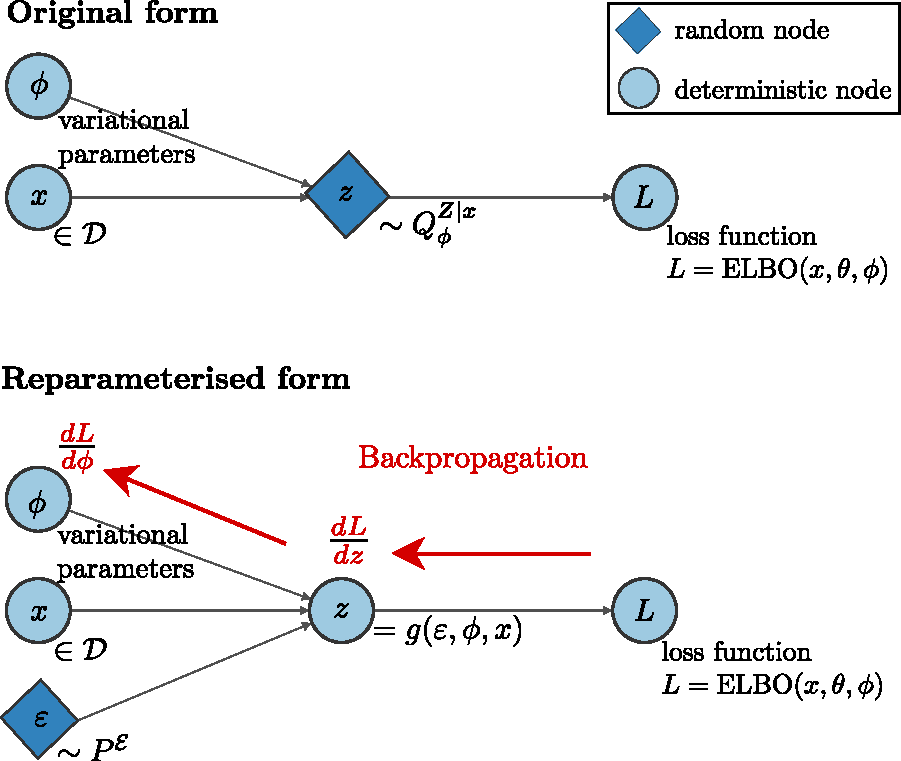
\includegraphics[height=8cm]{reparameterisation_trick.pdf}
	\caption{The reparameterisation trick. (adapted from \cite[p.~22]{Kingma2019})}
	\label{fig:reparam_trick}
\end{figure}

The complete training algorithm of the VAE, also termed \textbf{auto-encoding variational Bayes} algorithm by the original authors (\cite[p.~21]{Kingma2019}, \cite[p.~4]{Kingma2013}), is summarised in Algorithm 1. The training process is visualised in Figure~\ref{fig:VAE_with_reparam}.

\begin{algorithm}
	\SetAlgoLined
	\KwData{ \\Input: dataset $\mathcal{D} = \lbrace x_1,\dots, x_n\rbrace$, \\ 
		Inference model: family of variational posterior distributions $(\Q_{\phi}^{Z\mid x})_{\phi \in \Phi}$, \\
		Generative model: family of joint distributions $(\P_{\theta}^{X,Z})_{\theta\in \Theta}$}
	\KwResult{ \\ Learned parameters $(\theta, \phi)$ of the generative and inference model}
	
	$(\theta, \phi)\leftarrow$ Random initialization\;
	\While{SGD not converged}{
		Sample random minibatch of data $\mathcal{M} \sim \mathcal{D}$\;
		\For{each datapoint $x \in\mathcal{M}$}{
			Sample random noise $\varepsilon \sim \P^{\mathcal{E}}$\;
			Calculate $z = g(\varepsilon, \phi, x)$\;
		}{
		Compute (estimators of) $\elbo(\mathcal{M},\theta, \phi)$ and gradients $\nabla_{\theta, \phi}(\elbo(\mathcal{M},\theta, \phi))$\;
		Update parameters $\theta$ and $\phi$ using SGD optimiser\;
		}
	}
	\caption{Auto-encoding variational Bayes algorithm:	VAE training by stochastic optimisation of the ELBO}
	\label{algo-1}
\end{algorithm}

\begin{figure}
	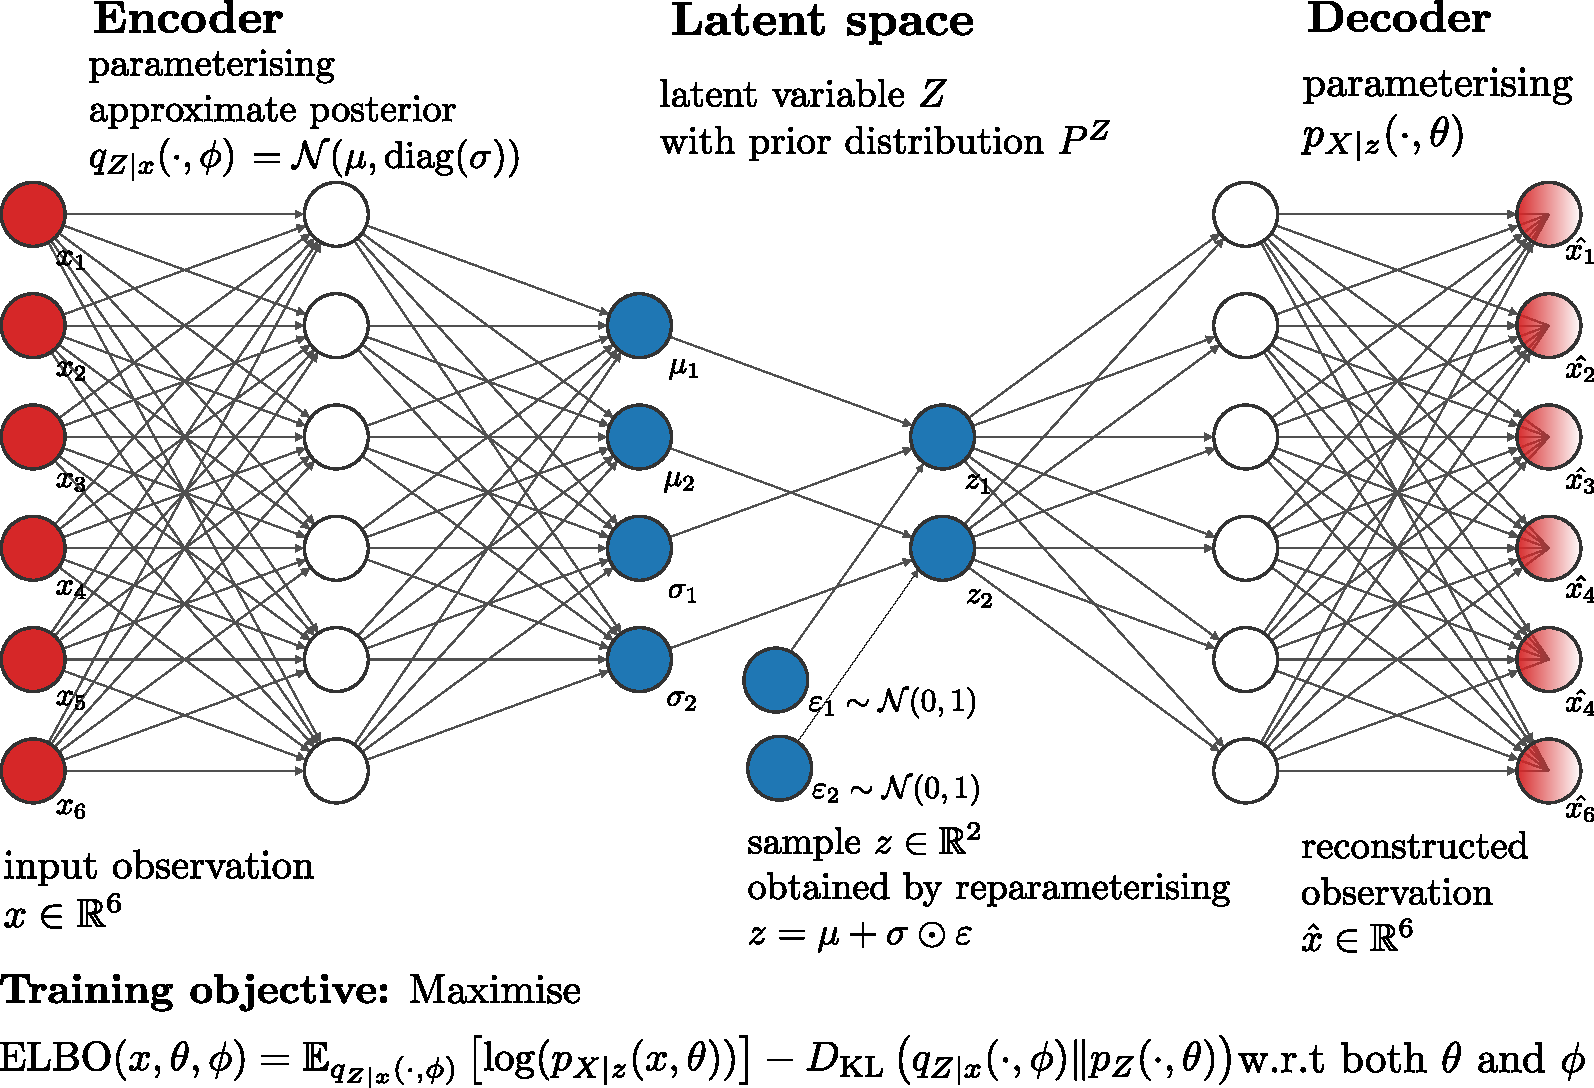
\includegraphics[height=9cm]{vae_with_reparameterisation.pdf}
	\caption{VAE training process with reparameterisation trick.}
	\label{fig:VAE_with_reparam}
\end{figure}

\subsection{Example: VAE with factorised Gaussian posterior}\label{sec:VAE-example_Gaussian_posterior}

In this section, I present a typical and commonly used example of a variational autoencoder with the standard choices for the distributions which enable an efficient computation of the ELBO and thus allow for efficient optimisation (\cite[pp.~24f.]{Kingma2019}, \cite[p.~5]{Kingma2013}). 

Let the prior over the latent variable $Z$ be given by a standard normal distribution, i.e., $Z\sim \P^Z = \mathcal{N}(0,I)$. In this case, the prior has no parameters and is thus not subject to any optimisation or change during training. Let $p_{X\mid z}(\cdot,\theta)$ be the density of a multivariate Gaussian (for real-valued data) or a Bernoulli distribution (for binary data). The distribution parameters $\theta$ are computed from realisations of the latent variable $Z$ with a neural network with a single hidden layer and non-linear activation function. 
In this case, the true posterior $p_{Z\mid x}(\cdot,\theta)$ is intractable. To approximate it, we choose a multivariate Gaussian distribution with mean $\mu \in \R^K$ and diagonal covariance matrix $\mathrm{diag}(\sigma^2)\in \R^{K\times K}$, where the variational parameters $(\mu, \sigma)$ are given by a neural network: 
\begin{equation}
\begin{split}
	(\mu, \log(\sigma)) &= \mathrm{EncoderNeuralNet}(x) \\
	q_{Z\mid x}(z,\phi) &= \prod_{k=1}^K q_{Z\mid x}(z_k,\phi) = \prod_{k=1}^K f_{\mathcal{N}(\mu,\mathrm{diag}(\sigma^2))}(z_k).
\end{split}
\end{equation}
This factorised Gaussian encoder corresponds to the mean-field approach from variational inference, where we also assume the members of the variational family to be mutually independent, such that the distribution factorises (\cite[pp.~7-10]{Blei}).

Choosing $\P^{\mathcal{E}} = \mathcal{N}(0,I)$, we can, for a sample $\varepsilon$ from $\P^{\mathcal{E}}$ and an observation $x$, obtain a sample $z$ from the posterior $\Q_{\phi}^{Z\mid x}$ via the reparameterisation 
$$
	z = \mu + \sigma \odot \varepsilon, 
$$
where $\odot$ denotes the element-wise product. Analogously to the Gaussian example, for any family of distribution defined by a "location" and a "scale", we can choose the standard distribution with location $0$ and scale $1$ for the auxiliary random variable $\mathcal{E}$ and set $z = \mathrm{location} + \mathrm{scale} \odot \varepsilon$. Additionally, also for families of posterior distributions $\left(q_{Z\mid x}(\cdot, \phi)\right)_{\phi\in\Phi}$ with a tractable inverse cumulative distribution function, a differentiable transformation $g$ and an auxiliary variable $\mathcal{E}$ can be chosen such that we can perform the reparameterisation trick (see for details \cite[p.~5]{Kingma2013}).

We have seen in (\ref{elbo_form_recerror_kldivtoprior}) that for any $x \in \mathcal{D}$
$$
	\elbo(x,\theta, \phi) = \E_{q_{Z\mid x}(\cdot, \phi)}[\log(p_{X\mid z}(x,\theta))] - \dkl(q_{Z\mid x}(\cdot, \phi) \Vert p_{Z}(\cdot,\theta)).
$$
The KL-divergence between two multivariate Gaussian distributions with $\mu_1,\mu_2 \in \R^K, \Sigma_1, \Sigma_2 \in \R^{K\times K}$ can be computed in closed form according to the formula
\begin{equation}\label{formula_explicit_KL}
\begin{split}
	\dkl(&\mathcal{N}(\mu_1,\Sigma_1)\Vert \mathcal{N}(\mu_2,\Sigma_2)) \\
	&= \frac{1}{2} \left(\mathrm{tr}(\Sigma_2^{-1}\Sigma_1) 
	+ (\mu_2 - \mu_1)^{\top}\Sigma_2^{-1}(\mu_2 - \mu_1) 
	- K 
	+ \log\left(\frac{\det(\Sigma_2)}{\det(\Sigma_1)}\right)\right).
\end{split}
\end{equation}
We thus obtain for the given choices of the prior and posterior the explicit expression
\begin{equation}
\begin{split}
	\dkl(q_{Z\mid x}(\cdot, \phi) \Vert p_Z)
	&= \dkl(\mathcal{N}(\mu,\mathrm{diag}(\sigma^2))\Vert \mathcal{N}(0,I)) \\
	&= \frac{1}{2}\left(\sum_{k=1}^K \sigma_k^2 + \mu_k^2 - 1 - \log\left(\sigma_k^2\right)\right).
\end{split}
\end{equation}

Using $L$ samples $z^{(1)}, \dots, z^{(L)}$ from the posterior by sampling $\varepsilon^{(1)}, \dots, \varepsilon^{(L)}$ from $\P^{\mathcal{E}} = \mathcal{N}(0,I)$ and calculating $z^{(l)} = \mu + \sigma \odot \varepsilon^{(l)}$, we thus obtain the following estimator for the ELBO at datapoint $x\in \mathcal{D}$:
\begin{equation}
	\elbo(x, \theta, \phi) = \frac{1}{2} \sum_{k=1}^{K}(1+\log(\sigma_k^2) - \mu_k^2 - \sigma_k^2) + \frac{1}{L}\sum_{l=1}^{L} \log(p_{\theta}(x\mid z^{(l)})).
\end{equation}

Here, the decoding term $\log(p_{X\mid z^{(l)}}(x,\theta))$ can be seen as a negative reconstruction error.
A theoretical justification of the particular choice of $q$ is the fact that the Gaussian distribution maximises the entropy, i.e., is the potentially most informative distribution to use if we have no prior knowledge on the structure desired (\cite[pp.~644f.]{Goodfellow2016}).

\section{Ordinary differential equations}\label{sec:ODEs}

Differential equations relate functions and one or more of their derivatives and thus form the paradigmatic concept to describe quantities changing over time. In the following sections, I  formally define differential equations and give basic central results about the existence and uniqueness of solutions. 

\subsection{Definitions}

\begin{definition}[{\cite[p.~27, Definition~1]{Perko2001}}]\label{def:ODE}
	Let $I\subset \R$ be an interval, $U\subset I\times \R^m$ open and $f:U\to\R^n$ a continuous function. Then, for an interval $J\subset I$, a function $x:J\to \R^n$ is called a \textbf{solution of the (ordinary) differential equation} $x' = f(\cdot, x)$ \textbf{on the interval $J$}, if $x$ is differentiable and
	$\frac{d}{dt} x(t) = f(t,x(t))$ for all $t\in J.$

	Additionally, given a $t_0\in J$ and $(t_0,x_0)\in U$, $x$ is called a \textbf{solution of the initial value problem} defined by $f$ and $(t_0,x_0)$ in $J$, if $x$ is a solution of the differential equation and $x(t_0) = x_0$, i.e., if
	\begin{equation*}
	\begin{split}
		\frac{d}{dt} x(t) &= f(t,x), \\
		x(t_0) &= x_0 \text{~for all~} t\in J.
	\end{split}
	\end{equation*} 
	\end{definition}

\begin{rmk}
	Definition~\ref{def:ODE} can be generalised to differential equations of higher orders: For an $n\in\N$, an open subset $U\subset I\times \R^n$ and a continuous function $f$ on $U$, a function $x\in\mathcal{C}^n(J)$ for $J\subset I$ is a solution of the differential equation $x^{(n)}(t) = f(t,x, x', x'',\dots, x^{(n-1)})$ in $J$, if 
	$$
	\tfrac{d^{(n)}}{dt} x(t) = f(t,x(t),\tfrac{d}{dt}x(t), \dots, \tfrac{d^{(n-1)}}{dt}x(t)) \text{~for all~} t\in J.
	$$
	Such a differential equation of order $n$ can always be reduced to a first-order differential equation as in Definition~\ref{def:ODE} by changing to the new set of variables $y = (x, x', x'', \dots, x^{(n-1)})$, which yields the first-order system
	\begin{equation*}
		\begin{split}
			y_1' &= y_2, \\
			&\;\;\vdots \\
			y_{n-1}' &= y_n \\
			y_n' &= f(t,y).
		\end{split}
	\end{equation*}
	Then, any function $x\in\mathcal{C}^n(J)$ is a solution of $x^{(n)}(t) = f(t,x, x', x'',\dots, x^{(n-1)})$ in $J$ if and only if the function $t\mapsto y(t)$ is a solution of the first-order differential equation $y' = f(\cdot, y)$ in $J$ (\cite[p.~7]{Teschl2012}). 
	
	For the corresponding initial value problem, let $(t_0,x_0,\dots, x_{n-1})\in U$ for $t_0\in J$. Then, $x\in\mathcal{C}^n(J)$ is a solution of the initial value problem defined by $f$ and $(t_0,x_0,\dots, x_{n-1})$ in $J$, if $x$ is a solution of the differential equation and additionally $x(t_0) = x_0, \frac{d}{dt}x(t_0) = x_1,\dots, \frac{d^{(n-1)}}{dt} x(t) = x_{n-1}$. 
	We thus see that for an initial value problem of order $n$, in addition to the initial value in $t_0$, the values of the first $n-1$ derivatives in $t_0$ have to be specified. 
\end{rmk}

\begin{rmk}
	Differential equations according to Definition~\ref{def:ODE} are called \textbf{ordinary differential equations (ODEs)}, because the solution function depends on only one variable that is denoted by $t$ in the definition. In contrast to that, equations specifying a relation between partial derivatives of a function of two or more variables or of a vector with two or more dimensions and the function itself are called \textbf{partial differential equations (PDEs)}. An example is the Laplace equation briefly mentioned in Section~\ref{sec:calculus_of_variation} given by 
	$$
	\Delta u(x_1,\dots, x_n) = \sum_{i=1}^{n} \frac{\partial^2}{\partial x_i^2}u(x_1,\dots, x_n) = 0.
	$$
\end{rmk}

\subsection{Existence and uniqueness of solutions}

The main result on the conditions under which initial value problems have solutions is given by the Picard-Lindelöf theorem, which proves local existence and uniqueness for a locally Lipschitz-continuous function $f$ defining the differential equation: 

\begin{theorem}[{Picard-Lindelöf, \cite[p.~38, Theorem~2.2]{Teschl2012}}]\label{thm:picard-lindelöf} Let $U\subset \R\times \R^m$ be an open subset, let $(t_0,x_0)\in U$ and $f:U\to\R^n$ be a continuous function. If $f$ is locally Lipschitz continuous in the second argument, uniformly with respect to the first argument, then there exists a unique local solution of the initial value problem defined by $f$ and $(t_0,x_0)$. More specifically, if $V = [t_0,t_0 + T]\times \overline{B_{\delta}(x_0)} \subset U$ and $M = \max_{(t,x)\in V} \vert f(t,x)\Vert$, the solution exists at least for $t\in [t_0,t_0 + T_0]$ and remains in $\overline{B_{\delta}(x_0)}$, where $T_0 = \min\lbrace T,\frac{\delta}{M}\rbrace$. The analoguous result holds for $[t_0-T,t_0]$.
	\begin{proof}
		I sketch the main steps of the proof and refer to \cite[pp.~36-38]{Teschl2012} for details. 
	 	The central idea is to reframe the statement of the theorem as a fixed-point equation of a functional on a complete metric space. Then, the claim follows from Banach's fixed-point theorem. 
	 	
		First, we observe that a function $x\in\mathcal{C}^1(J,\R^n)$ is a solution of the initial value problem defined by $f$ and $(t_0,x_0)$ in $J$ if and only if the function $x\in\mathcal{C}(J,\R^n)$ solves the integral equation (\cite[p.~36]{Teschl2012})
		$$	x(t) = x_0 + \int_{t_0}^{t} f(s,x(s)) ds.$$ 		
		Note that in order to satisfy the Lipschitz conditions, if suffices that $f\in \mathcal{C}^1(U)$: It then follows from the fact that any continuous function on a compact subset of a finite-dimensional real vector space attains its maximum in that subset (see \cite[p.~71f.]{Perko2001} for details) that for every compact set $V_0\subset U$ the number 
		$$ L = \sup_{(t,x)\neq(t,y)\in V_0} \frac{\vert f(t,x) - f(t,y) \vert}{\vert x-y\vert} $$
		is finite (\cite[p.~37]{Teschl2012}). 
		
		Next, we define the function space 
		$$ \mathcal{X}_I := \lbrace x\in \mathcal{C}(I,\R^n): \sup_{t\in I} \vert x(t) - x_0\vert <\delta\rbrace $$ 
		for some $\delta > 0$ and an interval $I\subset \R$, and a functional $K_I$ on $\mathcal{X}_I$ 
		\begin{equation*}
			\begin{split}
					K_I: \mathcal{X}_I &\to \mathcal{C}(I,\R^n), \\
					(t\mapsto x(t)) &\mapsto \left( t\mapsto T_I(x)(t) := x_0 + \int_{t_0}^{t}f(s,x(s)) ds\right).
			\end{split}
		\end{equation*}
		Then, according to our observation from the beginning of the proof, any function $x\in\mathcal{C}(I,\R^n)$ is a solution of the initial value problem defined by $f$ and $(t_0,x_0)$ on $I$ if and only if $x(t) = K_I(x)(t)$ for all $t\in I$, in other words, if and only if the function $x$ is a fixed point of $K_I$. 
		
		Defining $V := [t_0,T] \times \overline{B_{\delta}(x_0)} \subset U$ and denoting 
		$$M = \max_{(t,x)\in V} \vert f(t,x)\vert$$ 
		(the maximum exists by continuity of $f$ and compactness of $V$), we obtain 
		$$ \vert K_I(x)(t) - x_0 \vert \leq \int_{t_0}^ \vert f(s,x(s))\vert ds \leq tM$$
		for all $(t,x) \in V$. 
		Hence, if we define $$T_0 = \min \lbrace T,\frac{\delta}{M}\rbrace,$$ it follows that $T_0M\leq \delta$, and for all $t\leq T_0$, 
		$$ \vert K_I(x)(t) - x_0 \vert \leq T_0 M \leq \delta.$$
		Defining $I := [t_0, T_0]$, this implies that $K_I(\mathcal{X}_I) \subset K_I(\mathcal{X}_I)$. 
				
		We can now use the fact that $f$ is locally Lipschitz-continuous with respect to $x$ to show that for $I := [t_0, T_0]$, $K_I$ is a contraction on $\mathcal{X}_I$, i.e., $\sup_{t\in I}\vert (K_I(x))(t) - (K_I(y)(t))\vert \leq L T_0\sup_{t\in I}\vert x(t) - y(t)\vert$ (see for details \cite[pp.~40f.]{Teschl2012}). Since $X_I$ is complete with respect to the supremum norm, the existence of a unique fixed point and thus also the existence of a unique solution of the initial value problem now follows from Banach's fixed-point theorem (see, e.g., \cite[Theorem~2.1, p.~35]{Teschl2012}). 
	\end{proof}
\end{theorem}

\begin{rmk}
	With the help of Gronwall's inequality (\cite[p.~42f.]{Teschl2012}), it can be shown that the solution of an initial value problem depends continuously on the initial condition and the parameters of the system (see \cite[Section~2.3, pp.~79-84]{Perko2001} and \cite[Section~2.4, pp.~41-48]{Teschl2012}). 
	The existence of a solution can also be shown with Peano's existence theorem (\cite[Theorem~2.19, pp.~56f.]{Teschl2012}) under weaker conditions on the function $f$. Here, the proof is based on applying a fixed-point theorem by Schauder and the Arzela-Ascoli theorem.
\end{rmk}

\begin{rmk}\label{rmk:global_ODE_solution}
	If the coefficients of the differential equation grow at most linearly with respect to $x$, we can prove global existence of a solution: If in the setting of Theorem~\ref{thm:picard-lindelöf} for every $T>0$ there are constants $M(T), L(T)$ such that 
	$$ \vert f(t,x) \vert \leq M(T) + L(T)\vert x\vert, $$ the initial value problem defined by $f$ and $(t_0,x_0)$ has a unique solution defined for all $t\in \R$ (see \cite[Theorem~2.17, p.~53]{Teschl2012}).
\end{rmk}

\subsection{Linear ODEs}

\begin{definition}\label{def:linear_ODE}
	Let $I\subset \R$ be an interval. An ODE of the form 
	$$\frac{d}{dt} x(t) = A(t)x(t) + b(t)$$ for functions $A:I\to \R^{n\times n}, b: I\to \R^n$ is called \textbf{linear}. If $b\equiv 0$, the equation is called \textbf{homogeneuous}. 
\end{definition}

For homogeneuous linear ODEs with constant coefficients, i.e. with $A(t)\equiv A \in \R^{n\times n}$ for all $t\in I$, we can derive an explicit solution with the help of the following definition: 

\begin{definition}[{\cite[p.~60]{Teschl2012}}]\label{def:matrix-exponential}
	For a matrix $B\in \R^{n\times n}$, we define the \textbf{matrix exponential}
	$$
	\exp(B) := \sum_{k=0}^{\infty} \frac{B^k}{k!}. 
	$$
\end{definition}

\begin{theorem}\label{thm:ODE-solution_linear_homogenous_multidimensional}
	Let $B\in \R^{n\times n}$ be a matrix, let $J\in \R^{n\times n}$ be the Jordan normal form of $B$, such that $J = S^{-1}BS$ for a matrix $S\in \R^{n\times n}$. Then, for $f(t,x) = Bx$ and $(t_0,x_0)\in \R\times \R^n$, the solution of the initial value problem defined by $f$ and $(t_0,x_0)$ on $\R$ is given by the function 
	$$
	x(t) = \exp(B(t-t_0))x_0 = S\exp(J(t-t_0))S^{-1}x_0. 
	$$
	\begin{proof}
		We can explicitly calculate that $x(t) = \exp(B(t-t_0))x_0$ solves the initial value problem. The second equality follows from the properties of the matrix exponential (for details see \cite[Section~3.1, pp.~59-64]{Teschl2012}). 
		%Using the properties of the Jordan normal form, we can explicitly calculate $\exp(Jt)$. 
	\end{proof}
\end{theorem}

\begin{rmk}
	For a general linear homogeneous first-order systems, i.e., a system where the coefficient matrix $A$ can depend on $t$, if $A\in \mathcal{C}(I,\R^{n\times n})$, existence and uniqueness of a solution on the entire interval $I$ follow from the result mentioned in Remark~\ref{rmk:global_ODE_solution} by choosing $L(T) = \max_{[0,T]}\Vert A(t)\Vert$ for every $T\in I$. To give an explicit form of the solution, it is neccessary to define the right generalisation of the expression $\exp((t-t_0)A)$. This is developed, e.g., in \cite[Section~3.4, pp.~80-86]{Teschl2012}. 
\end{rmk}

\chapter{Methods}\label{chap:methods}
\fancyhead[LO]{\nouppercase{\leftmark}}

\section{Modelling smooth latent dynamics within a VAE framework}\label{sec:methods-generalintro}

We have seen that VAEs can infer lower-dimensional representations of the central factors of variation in a dataset. In the simulated data setting outlined in Chapter~\ref{chap:intro}, we have such an underlying low-dimensional dynamical system from which the observations are generated.
In an epidemiological cohort study such as the NAKO, we are typically interested in the underlying concept of the study participants' general condition and their mental and physical health status and try to access that health status, being a complex phenotype, by taking a multitude of individual measurements. It is thus plausible to assume the presence of groups of variables that jointly describe a more general underlying concept, e.g., we can imagine to collect data on individual's BMI, frequency of physical acticity, resting pulse rate and dietary habits all contributing to a latent representation of the individual's general physical fitness. 
Since we do not know specifically in what way single variables contribute to which part of a latent structure, the VAE provides a viable tool to infer such a latent representation directly from data in an unsupervised way, allowing for potentially complex, non-linear interactions. My model to infer the underlying lower-dimensional development patterns is therefore based on a VAE architecture.

The data are viewed as snapshots from a process evolving continuously over time that is observed with measurement noise. Consequently, also the underlying latent structure can be assumed to consist of dynamics changing smoothly over time and the latent space-representation has to be constrained to describe such smooth temporal development patterns. In my model, I formulate this constraint as the assumption that the latent space can be described by a system of differential equations that capture the basic dynamics underlying the observations.
This implies that the latent variable $Z$ should represent both a random variable and a function changing over time, i.e., a stochastic process.
Regarding the elements of stochasticity in the observed process, I assume a "true", inherently deterministic underlying dynamic process and a random force not acting on the process itself, but on a noisy observation of it. That observation is governed by some level of uncertainty, which I assume to be independent of the observation time. 
As a result, the latent space of the VAE model should encode a low-dimensional representation of the data that matches a smooth trajectory, with a stochastic element accounting for the uncertainty in the generating process of observations from an inherently deterministic underlying trajectory. 
This implies to model the stochasticity of the process as the random measurement error in the observations that can be assumed to be distributed according to $\mathcal{N}(0,\sigma^2)$. 
Consequently, I employ a Gaussian prior and posterior for the latent random variable $Z$. Here, the posterior mean represents its value according to the deterministic trajectory described by the ODE system, while the variance accounts for the uncertainty in the observation of that value. 

Summing up, I describe the true deterministic process from which data are generated as an ODE system imposed on the latent space formulated in terms of the posterior mean $\mu_{\mathrm{post}}$ of $\Q^{Z\mid x} = \mathcal{N}(\mu_{\mathrm{post}}, \sigma_{\mathrm{post}}^2)$ to account for the assumption of modelling a deterministic process with a random element in its observation, but not the temporal development itself. I therefore constrain the latent space to describe smooth dynamics by solving an ODE system for the posterior mean. To model the stochasticity of the measurement process, I subsequently sample $z$ from the posterior distribution according to smooth dynamics after solving the ODE and decode it to the data space to obtain a reconstructed observation.

\section{Fitting individual ODE parameters with baseline variables}\label{sec:methods-ODEparamswithbaselineinfo}

As a further important feature, the model should be capable of extracting individual-specific development patterns, i.e., to fit individual ODE systems to the posterior mean of the latent representation. Since this representation should recover the main factors of variation that govern the observed developments, I define a low-dimensional system of ODEs with one equation for every dimension of the latent representation that can be thought of as an underlying common trend shared by several variables in the original dataset.  

The general structure of the ODE is explicitly specified as a linear system in Chapter~\ref{chap:applications}, Sections~\ref{sec:apps-linear2p} and \ref{sec:apps-linear4p} or as a non-linear system in Chapter~\ref{chap:applications}, Section~\ref{sec:apps-nonlinear2p}, but the parameters of the pre-defined system are determined individually for each input observation to account for different development patterns in the same set of measured variables.
To infer such an individual-specific set of ODE parameters, I employ the additional variables measured only at the baseline timepoint, assuming that this more extensive characterisation carries information about each individual's development. 
Since I assume it to be unknown how they specifically relate to the individual ODE parameters, I employ an additional neural network to map the observations of the baseline variable to a set of ODE parameters for each individual. I train this network jointly with the VAE model, since the model should find a latent representation matching the assumption that the latent space can be described by an ODE system. By training jointly, the ODE structure imposed on the latent space is allowed to influence the VAE training and guide the model to find an appropriate latent representation.

As an example to motivate this method, we can imagine to measure several time-dependent variables describing lung function and at baseline also collect information about chronic lung diseases, age, physical activity and smoking habits. Then, these additional baseline measurements can potentially be informative about the development of each individual's lung function. More generally, if there are groups of individuals sharing common development trends, e.g., chain smokers, the baseline variables could contain information from which an individual's group membership can be deduced. 

\section{Derivation of the ODE-VAE training objective}\label{sec:methods-ODE-VAEtraining}

I now formalise my method by describing the training process of the model and deriving an adapted version of the ELBO to define the loss function. 

The dataset $\mathcal{D} = \lbrace x_1,\dots, x_n\rbrace$ includes $n$ observations that each consist of two measurements of $p$ variables, i.e. $x_i = (x_i\tn \quad x_i\te) \in \R^{p\times 2}$ with $x_i^{t_j}= (x_{i,1}^{t_j}, \dots, x_{i,p}^{t_j})^{\top} \in \R^{p}$ for $j=0,1$.
The encoder part of the VAE maps an input observation $x_i$ column-wise to the mean  $\mu_i= (\mu_i\tn \quad \mu_i\te) \in \R^{k\times 2}$ and standard deviation $\sigma_i = (\sigma_i\tn \quad \sigma_i\te) \in \R^{k\times 2}$ of the posterior distribution $\mathbb{Q}^{Z\mid x_i} = \mathcal{N}(\mu_i,\sigma_i^2)$, where $k$ is the dimension of the latent space.

For each individual $i$, I denote with $y_{i,1},\dots, y_{i,q}$ the measurements of the additional baseline variables used to infer the parameters of the ODE system in latent space. A neural network that I refer to as the \textbf{ODE-net} maps the corresponding observation $y_i = (y_{i,1}, \dots, y_{i,q})^{\top} \in \R^q$ to a set of individual ODE parameters $\eta_i \in \mathbb{R}^l$, with $l$ being the number of parameters of the ODE system. 

The latent space dynamics are given by a pre-specified function $f(\mu_i(t), t, \eta_i)$ that describes either a homogeneous two-dimensional linear ODE system or a non-linear Lotka-Volterra ODE system. 
The parameters of this ODE system are inferred from the individual-specific baseline measurements with the ODE-net.
Then, we can solve the initial value problem 
\begin{equation*}
\begin{split}
	\frac{d}{dt} \mu_i(t) &= f(\mu_i(t), t, \eta_i)\\
	\mu_i(t_0) &= \mu_i\tn
\end{split}
\end{equation*}
at $t_i^{1}$, the time point of the individual's second measurement, and obtain a vector $\widetilde{\mu_i}\te = \mathrm{ODESolve}(f(\mu_i(t), t, \eta_i), \mu_i\tn, t_i^{1}) \in \R^k$. We now define $\widetilde{\mu_i} := (\mu_i\tn \quad \widetilde{\mu_i}\te)$ as the mean of the posterior distribution constrained to a smooth dynamic and draw a sample $z_i\sim \widetilde{\Q}^{Z\mid x_i}_{\eta_i,\phi} = \mathcal{N}(\widetilde{\mu_i}, \sigma_i^2)$ from the approximate posterior. Subsequently, $z_i$ is passed to the decoder of the VAE that parameterises $P_{\theta}^{X\mid z_i}$, the conditional distribution of the data given a sample of the posterior, to obtain a reconstructed observation $\widehat{x_i}$ as a sample from $P_{\theta}^{X\mid z_i}$. 

To define a training objective for jointly optimising the VAE model constrained to smooth latent space dynamics and the ODE-net, I adapt the ELBO of (\ref{elbo-as-function-of-theta-and-phi}): To learn the latent space dynamics according to the ODE system jointly with the network supplying the parameters of this system, the posterior mean as obtained from solving the ODE is used. Because this mean and therefore also the posterior distribution depends on the parameters $\eta_i$ of the individual's ODE system, we thereby introduce dependence of the ELBO on the ODE parameters and hence provide feedback for learning the weights and biases of the ODE-net:
\begin{equation}
\begin{split}
\mathrm{ELBO}_{\mathrm{smooth}}(x_i\tn, x_i\te, \eta_i, \theta, \phi) &= -D_{\mathrm{KL}}(\widetilde{q}_{Z\mid x_i\tn, x_i\te}(\cdot, \eta_i, \phi) \Vert p_Z(\cdot,\theta)) \\ 
&+ \E_{\widetilde{q}}[\log(p_{X\mid z_i\tn, z_i\te}(x_i\tn, x_i\te,\theta))],
\end{split}
\end{equation}
where $\widetilde{q}$ is used as an abbreviation for $\widetilde{q}_{Z\mid x_i\tn, x_i\te}(\cdot, \eta_i, \phi)$ in the expectation.
Since the solution of an ODE is uniquely defined (if it exists) by the function specifying the derivative and the initial value according to Theorem~\ref{thm:picard-lindelöf} (Picard-Lindelöf), the ODE solution $\widetilde{\mu_i}\te$ depends exclusively on the initial value $\mu_i\tn$ and the ODE parameters $\eta_i$, but not on the observations at the second time point $x_i\te$. 
It follows that the posterior distribution $\widetilde{\Q}^{Z\mid x_i}_{\eta_i, \phi}$ is independent of $x_i\te$, hence $\widetilde{q}_{Z\mid x_i\tn, x_i\te}(\cdot, \eta_i, \phi) = \widetilde{q}_{Z\mid x_i\tn}(\cdot, \eta_i, \phi)$. To improve the capability of the model to still reconstruct $x_i\te$ along with $x_i\tn$ and to provide feedback for the encoder weights and biases with respect to $x_i\te$, the loss is augmented with the squared euclidean distance between $\mu_i\te$ as obtained from directly passing $x_i\te$ through the encoder and $\widetilde{\mu_i}\te$ as obtained from solving the ODE.
By minimising that distance, the posterior distribution from the encoder $q_{Z\mid x_i\tn, x_i\te}(\cdot,\phi)$ is brought to match the posterior distribution $\widetilde{q}_{Z\mid x_i\tn}(\cdot, \eta_i, \phi)$ constrained to smooth latent space dynamics. In that way, the model is encouraged to encode the data from both measurement time points into a lower-dimensional representation that matches the smooth structure reinforced by the ODE system even before applying the ODE solving step.
Since the encoder posterior $q_{Z\mid x_i\tn, x_i\te}(\cdot,\phi)$ directly depends on $x_i\te$, bringing it close to $\widetilde{q}_{Z\mid x_i\tn}(\cdot, \eta_i, \phi)$ implicitly provides feedback from $x_i\te$ on $\widetilde{\mu_i}\te$ and thus achieves an implicit conditioning of $\widetilde{q}_{Z\mid x_i\tn}(\cdot, \eta_i, \phi)$ on $x_i\te$. Adding the term with a weighting factor of $\alpha\in[0,1]$ results in the final loss
\begin{equation} \label{finalELBO}
\begin{split}
\mathcal{L}(x_i\tn, x_i\te, \eta_i, \theta, \phi) &= -\mathrm{ELBO}_{\mathrm{smooth}}(x_i\tn, x_i\te, \eta_i, \theta, \phi) + \alpha\Vert\mu_i\te - \widetilde{\mu_i}\te\Vert_2^2 \\
=&\dkl(\widetilde{q}_{Z\mid x_i\tn, x_i\te}(\cdot, \eta_i, \phi) \Vert p_Z(\cdot,\theta)) \\
&- \E_{\widetilde{q}}[\log(p_{X\mid z_i\tn, z_i\te}(x_i\tn, x_i\te,\theta))]\\
&+ \alpha\Vert\mu_i\te - \widetilde{\mu_i}\te)\Vert_2^2.
\end{split}
\end{equation}

Note that by minimising $\mathcal{L}$, we still maximise a lower bound on the data likelihood, since the negative loss equals the ELBO with a positive term subtracted. Heuristically, by jointly maximising the ELBO and minimising the distance of $\mu_i\te$ and $\widetilde{\mu_i}\te$ via minimising $\mathcal{L}$, we can even obtain a lower bound closer to the true data likelihood due to the implicit conditioning of the smooth posterior $\widetilde{\Q}_{\eta_i, \phi}$ on $x_i\te$, which potentially leads to a better reconstruction error while still maintaining a smooth dynamic structure of the latent state. 
Figure~\ref{fig:node_vae_architecture_draft} provides a graphical overview of my model and its training process. 

\begin{figure}[H]
	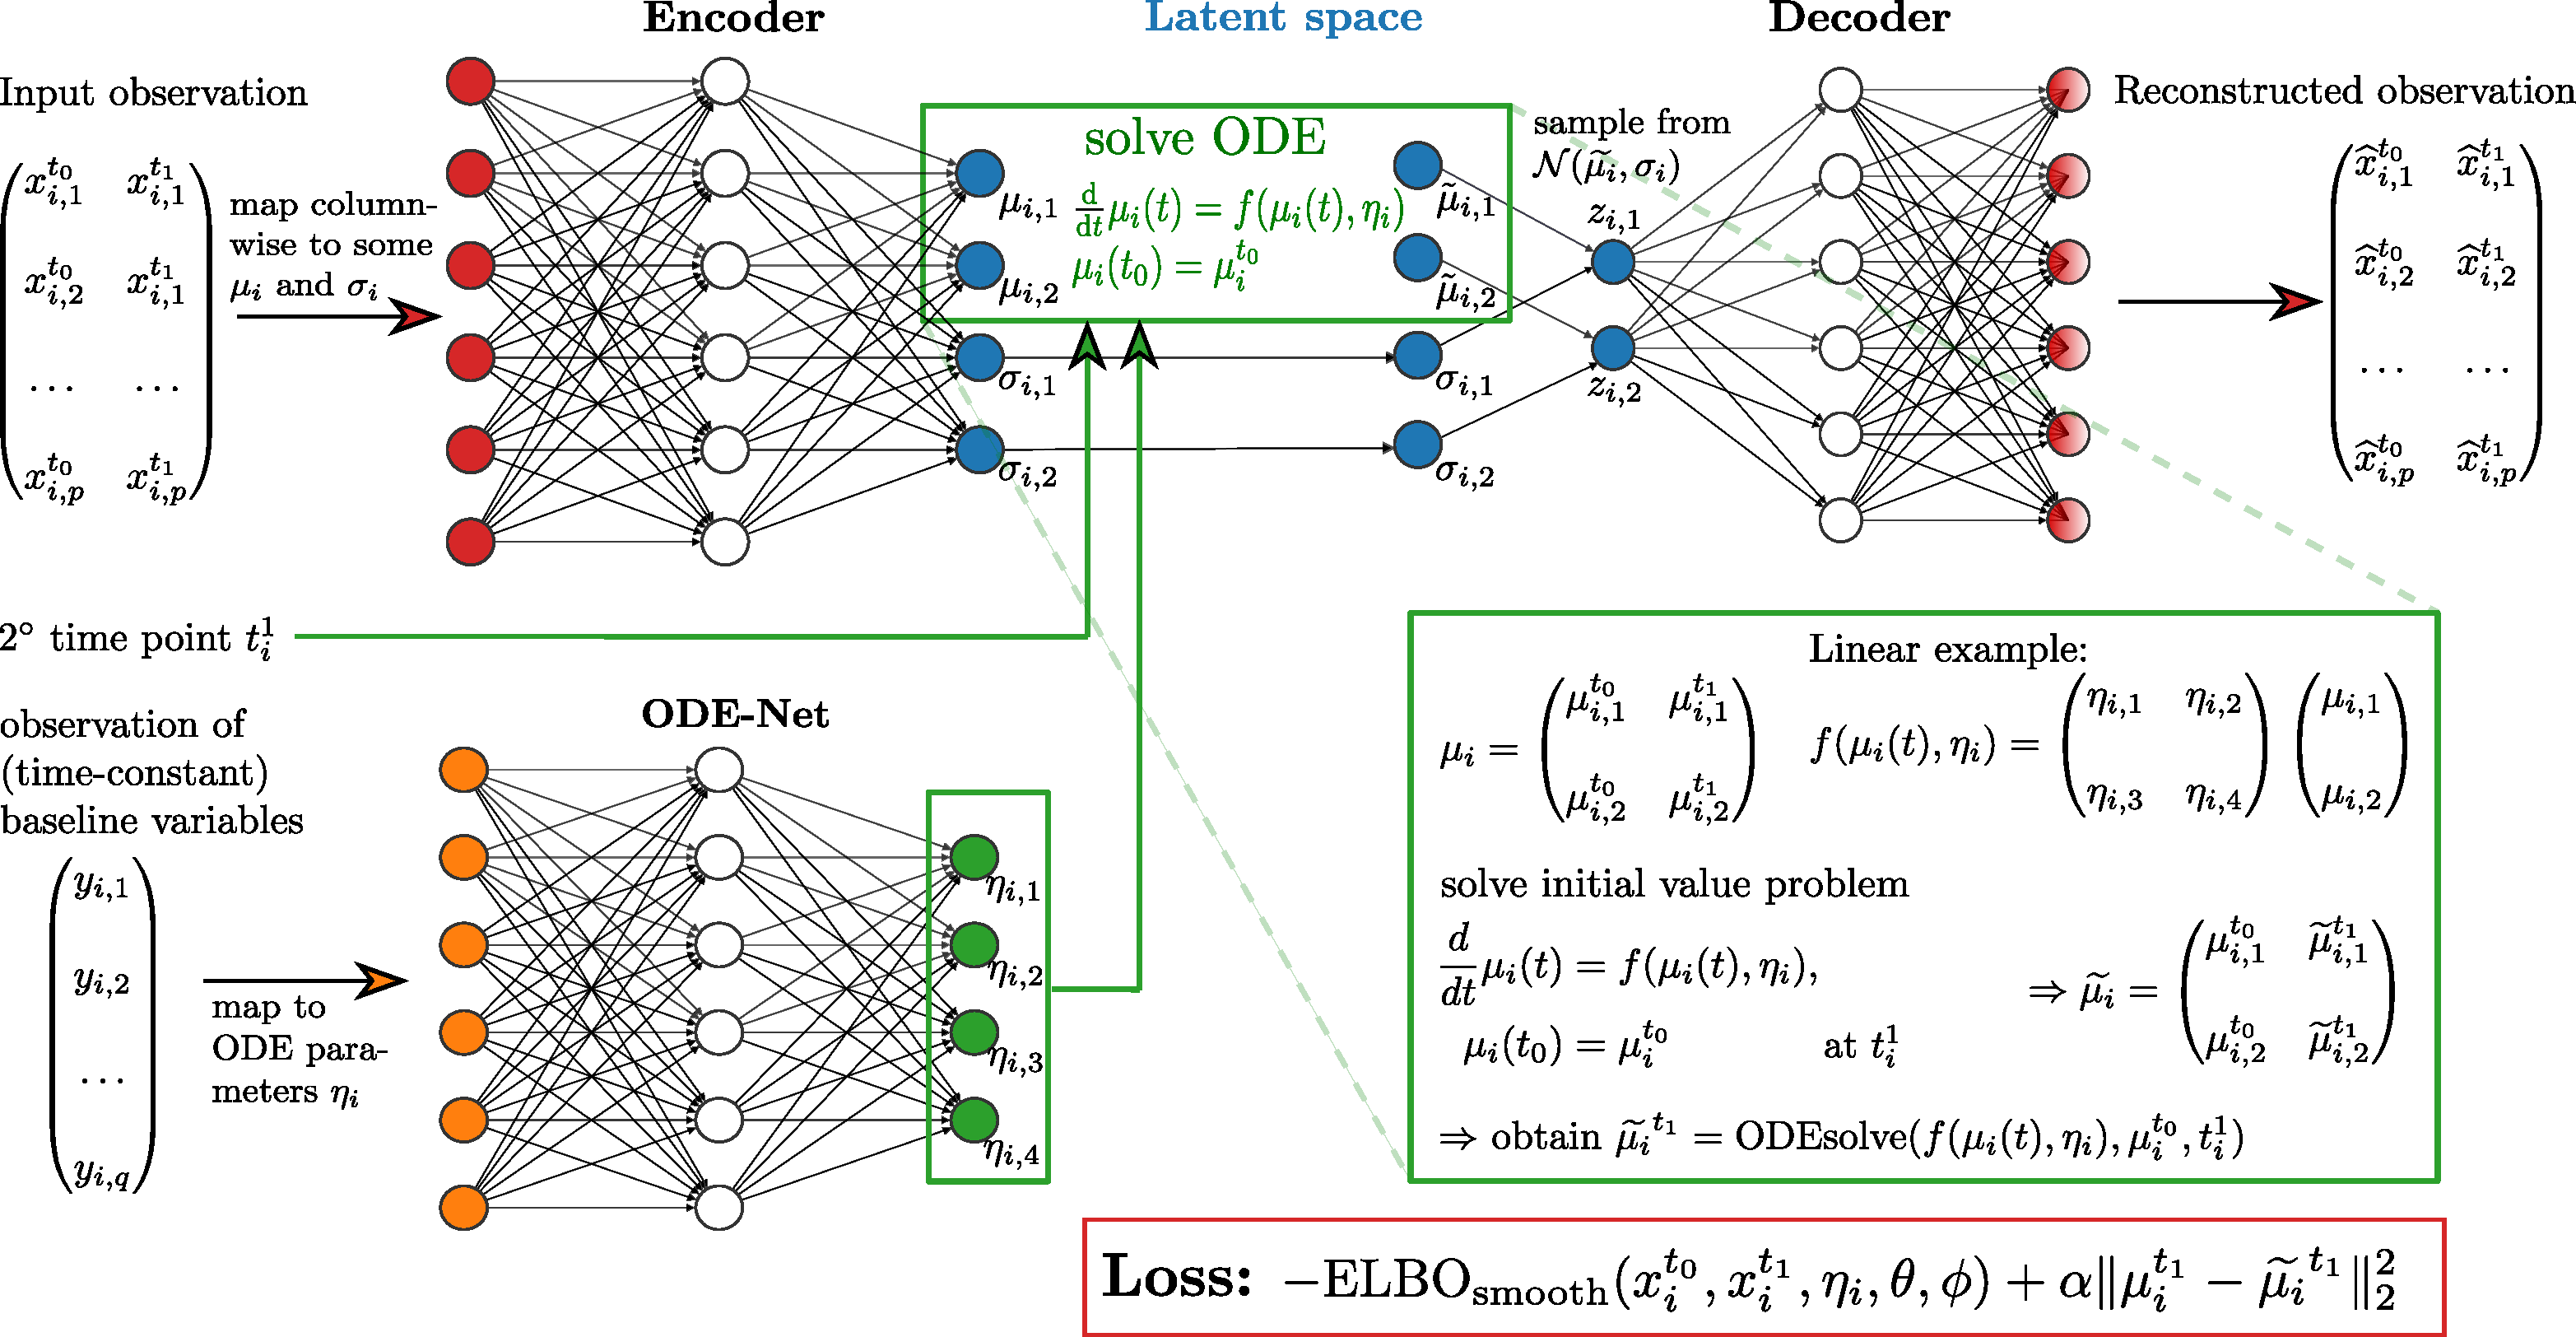
\includegraphics[width=\linewidth]{ODE_VAE_archichtecture.pdf}
	\caption{Overview of model architecture and training.}
	\label{fig:node_vae_architecture_draft}
\end{figure}

\section{Model extension: training on batches of similar individuals}\label{sec:methods-minibatches}

\subsection{Time sparsity and notion of similarity}\label{sec:methods-batches-generalintro}

A major challenge for my approach of modelling dynamic processes with individual-specific ODE systems in latent space is the strong sparsity and irregularity of the time grid with only two observations for every individual, which implies constraints on the complexity of ODE systems that can be fitted with these data. While it is natural to assume that two time points allow to estimate two unknown ODE parameters for each individual, the model should optimally also capture more complex development patterns.
% with our model and to include more parameters in the ODE systems. 
%In our applications, however, we noted that if the number of parameters exceeds the number of time points each individual is observed at, the systems are underdetermined and the model does not pick up on individual development patterns any more. 
%Their combination of all second time point measurements in the batch then serves as proxy information on the common dynamics at multiple time points,

This is achieved with an extension of my method: To every individual, a batch of individuals with similar underlying development patterns is assigned. Then, the combination of all their second time point measurements can be used as proxy information on the common dynamics at multiple time points. Thus, each observation is enriched with a group of similar ones observed at different time points and the irregularity of the time grid is exploited to address the problem of strong time sparsity, which ultimately allows to model more complex development patterns. 

More specifically, first a measure of similarity has to be defined to identify individuals with similar development patterns. Since each individual is observed at a different second time point, their measurements cannot be directly compared in data space. Additionally, if the random measurement noise in the observations superimposes the true underlying developments, it can be impossible to identify similar trajectories from the data alone.

Figure~\ref{fig:minibatches_explanation} provides an illustration of the batch assignment: For each individual, the observations are generated from one of two different underlying development patterns with a moderate level of noise. The original underlying pattern is indicated by the frame colour of each panel (violet/green). The development of the individual at the top is different from the left one in the second row, but similar to the right one in the third row.
However, it is challenging to judge from these observations alone whether the right individual in the second row and the left in the third row are based on different underlying development patterns. This becomes clear only after passing each observation through the encoder and comparing the latent representation of the trajectories: In latent space, depicted in the middle part of the figure, we can clearly distinguish the two general development patterns. 

Consequently, I define the similarity of individuals based on their latent trajectories represented by the solution of each individual's ODE system in latent space. To infer for a given individual a batch of similar ones, I therefore first pass all observations through the VAE encoder. In the latent space of ODE solutions, I calculate the $L^2$-norm of distances of the ODE solutions and sort individuals according to distance to the reference individual. 
Additionally, I use a kernel to weigh the individuals with respect to their similarity to the reference individual. The complete method is formalised in the following sections.

\begin{figure}
	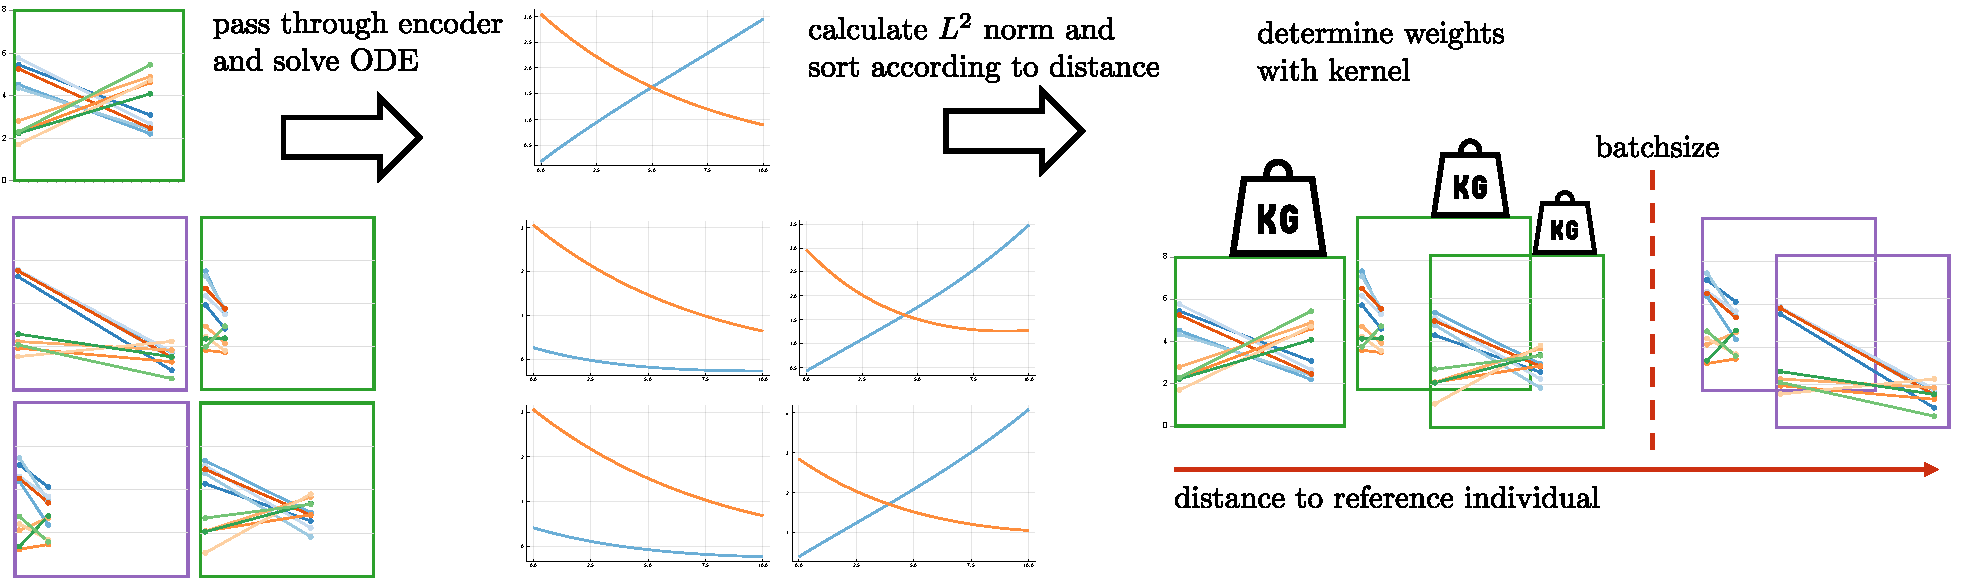
\includegraphics[width=\linewidth]{minibatches_explanation_figure_thesis.pdf}
	\caption{Assigning to an individual a batch of similar ones.}
	\label{fig:minibatches_explanation}
\end{figure}

\subsection{Defining an iterative optimisation framework}\label{sec:methods-batches-EMprocedure}

The proposed notion of similarity between individuals refers to the similarity not of their observed measurements, but of their unobserved latent trajectories, i.e., their ODE solutions in the latent space of the ODE-VAE model, that should ideally reflect the true underlying development patterns. However, inferring such a latent representation that recovers the true ODE system underlying every individual's observed measurements is the objective of the training process that we aim to improved by using the batches of similar individuals in the first place. 
In other words, a notion of similarity based on the underlying trajectories is needed to group individuals to train the model, i.e., to find a latent representation recovering the true dynamics, but at the same time such a meaningful latent representation is already needed to accurately infer individuals' similarity. 

To overcome this problem, I introduce an iterative optimisation framework that alternates between the assignment of batches of similar individuals and the joint training of the ODE-VAE model.
In this way, the latent representation of the trajectories are improved iteratively, so that they more closely reflect the true developments and individuals can be grouped more accurately based on these trajectories. Training on these groups -- that more accurately capture the similarity of the underlying patterns -- in turn improves individuals' latent representations due to better proxy information at other time points from the batch. This results in an overall training method that resembles an expectation-maximisation framework (Chapter~\ref{chap:background}, Section~\ref{sec:bayesian_inference}).\\ 

\subsubsection{Assigning a batch to each individual}

To group individuals in batches based on the similarity of their ODE solutions in latent space, every individual observation $x_i\in \mathcal{D}, i\in\lbrace1,\dots, n\rbrace$ is first passed through the VAE encoder to obtain an approximate posterior mean $\mu_i= (\mu_i\tn \quad \mu_i\te) \in \R^{k\times 2}$ and variance $\sigma_i = (\sigma_i\tn \quad \sigma_i\te) \in \R^{k\times 2}$ as in Section~\ref{sec:methods-ODE-VAEtraining}. Also, the respective baseline measurements $y_i$ are passed through the ODE-net to obtain a set of individual ODE parameters $\eta_i$. Next, each individual's ODE system as defined by the function $f$ denoting the common ODE structure and the individual parameters $\eta_i$ is solved to obtain for each individual the posterior mean according to smooth dynamics as a function of $t$:
$$\mu_i(t) = \mathrm{ODEsolve}(f(\mu_i(t), t, \eta_i)).$$
For a $T \in \R$, it holds that for all $i$, $\mu_{i} \in L^2([t_0,T])$. Now, we calculate a symmetric distance matrix 
$$D= (d_{i,j})_{i,j=1,\dots,n} = \left(\Vert \mu_i - \mu_j\Vert_{L^2([t_0,T])}\right)_{i,j=1,\dots,n}$$ 
where the $i,j$-th entry denotes the distance in $L^2$-norm between the ODE solutions $\mu_i(t)$ and $\mu_j(t)$ of individuals $i$ and $j$. In my implementation, the ODE solutions are evaluated at a fixed grid of $m+1$ time points $t_0,\dots, t_m$ to approximate the $L^2$-integral:
\begin{equation}\label{eq:discretisationl2norm}
	d_{i,j} = \left( \frac{1}{m} \sum_{t=t_0}^{t_m} \Vert \mu_i(t) - \mu_j(t)\Vert_2^2 \right)^{\frac{1}{2}}.
\end{equation}
For a pre-defined batch size of $b$, to each individual the $(b-1)$ individuals closest to that reference individual are assigned: 
Let $i\in\lbrace1,\dots, n\rbrace$ be the index of the reference individual. Of course, $d_{i,i}= 0$. The remaining entries in row $i$ are sorted such that $d_{i,j_1} \leq d_{i,j_2} \leq \dots \leq d_{i,j_{n-1}}$ where $j_k \in \lbrace 1,\dots , i-1, i+1, \dots, n\rbrace$ for $k=1,\dots, n-1$. 
For any $a <n$, the indices $j_1,\dots, j_a$ now denote the indices of the $a$ closest individuals to the reference individual. Thus, a batch $B_i$ of the $b-1$ individuals closest to $x_i$ can be defined by setting 
$$
B_i = \lbrace x_i, x_{j_1},\dots, x_{j_{b-1}} \rbrace.
$$ 
The closer an individual is to the reference individual, the more similar is its underlying development pattern. This implies that also the substistute information provided by that individual is potentially more accurate and should thus be regarded as more important for the training of the specific batch. To account for that, each individual in the batch is weighted according to its calculated distance to the reference individual. Specifically, weights $w_i, w_{j_1},\dots, w_{j_{b-1}}$ are determined for each individual in the batch $B_i$ with a smoothing kernel $K_h$, such that 
\begin{equation}\label{kernel-weights}
	w_k = \frac{K_h(d_{i,k})}{\sum_{k=i,j_1,\dots, j_{b-1}} K_h(d_{i,k})} \quad \text{for all } k=i,j_1,\dots, j_{b-1}. 
\end{equation}
The kernel is defined as the tricube function given by
$$
K(x) = \begin{cases}
(1-\mid x\mid^3)^3 & \mid x\mid \leq 1, \\
0 & \ \mathrm{else}
\end{cases}
$$
and can be scaled with the bandwidth parameter $h$ by defining  $K_h(x) = \frac{1}{h} K(\frac{x}{h})$. 

\subsubsection{Adapting the ODE-VAE loss to training on batches}

Having determined for each individual a batch of individuals exhibiting similar temporal development patterns, the ODE-VAE model is trained on the resulting batches in order to improve the estimates of the variational parameters of the approximate posterior $\phi$, the model parameters $\theta$ and the individual ODE parameters $\eta_i$ with respect to the training objective $\mathcal{L}(x_i\tn, x_i\te, \eta_i,\theta,\phi)$ of (\ref{finalELBO}): 

For each individual in the batch, the respective loss value is calculated as described in Section~\ref{sec:methods-ODE-VAEtraining}. 
Since for each individual the solution at the individual-specific second measurement time point is used to calculate its loss, those additional values now serve as proxy information for measurements at more time points (one from each individual in the batch) of the reference individual. To use them to enrich this reference individual's information and stabilise the gradient of its loss function, we derive a common loss value for the entire batch as the weighted average of individual loss values, using the weights derived from the distance matrix of the first step. The final training objective is thus given by the loss of each batch $B_i$, $i=1,\dots, n$: 
\begin{equation}\label{batches-finalcommonloss}
	\mathcal{L}_{\mathrm{batch}}(B_i, (\eta_k)_{k=i,j_1,\dots, j_{b-1}}, \theta,\phi) = \sum_{k=i,j_1,\dots, j_{b-1}} w_k \cdot \mathcal{L}(x_k\tn, x_k\te, \eta_k,\theta,\phi).
\end{equation} 

The weighting approach ensures that the individuals contributing most strongly to the common loss are the ones which best match the trajectory of the reference individual and therefore provide a good proxy for the observations of the reference individual at additional time points. 

The overall method to train the ODE-VAE model on batches now consists of iteratively applying the two steps and is summarised in Algorithm~\ref{algo-batches}.

\begin{algorithm}
	\SetAlgoLined
	\KwData{ \\ Dataset $\mathcal{D} = \lbrace x_1,\dots, x_n\rbrace$ of time-dependent variables, \\ additional baseline variables $y_1,\dots, y_n$ \\ 
		Inference model: family of approximate variational posterior distributions $(Q_{\phi}^{Z\mid x})_{\phi \in \Phi} = (\mathcal{N}(\mu,\sigma^2))_{(\mu,\sigma^2)\in\R^{k\times 2}\times \R^{k\times 2}}$, \\
		Generative model: family of joint distributions $(P_{\theta}^{X,Z})_{\theta\in \Theta}$, \\
		Function $f: \R^k \times \R \times \R^l \to \R^k$ defining general structure of latent ODE system, parameterised by $\eta \in \R^l$ }
	\KwResult{ \\ Learned parameters $(\theta, \phi)$ of the generative and inference model, individual-specific ODE parameters $\eta_i$}
	
	$(\theta, \phi, \mathrm{ODEnet} )\leftarrow$ Random initialization\;
	\While{SGD not converged}{
		\For{each datapoint $x_i \in\mathcal{D}$}{
			Compute $\eta_i = \mathrm{ODEnet}(y_i)$ \;
			Compute $\mu_i(t) = \mathrm{ODEsolve}(f(\mu(t),t,\eta_i),\mu_i\tn)$ \;
			Compute distance matrix $D = (\Vert \mu_i(t) - \mu_j(t)\Vert_{L^2})_{i,j=1,\dots, n}$ \;
			Sort $d_{i,j_1} \leq d_{i,j_2} \leq \dots \leq d_{i,j_{n-1}}$, $j_k \in \lbrace 1,\dots , i-1, i+1, \dots, n\rbrace$\;
			Define $B_i = \lbrace x_i, x_{j_1},\dots, x_{j_{b-1}} \rbrace$\; 
			Calculate $w_k = \frac{K_h(d_{i,k})}{\sum_{k=i,j_1,\dots, j_{b-1}} K_h(d_{i,k})}$\;
		}
		\For{each batch $B_i = \lbrace x_i, x_{j_1},\dots, x_{j_{b-1}} \rbrace$}{
			\For{each $x\in B_i$}{
			Sample random noise $\varepsilon \sim \P^{\mathcal{E}}$ and compute $z = g(\varepsilon, \phi, x)$\;
			Compute $\mathcal{L}(x_k\tn, x_k\te, \eta_k,\theta,\phi)$\;}
			Compute $\mathcal{L}_{\mathrm{batch}}(B_i, (\eta_k)_{k=i,j_1,\dots, j_{b-1}}, \theta,\phi) = \sum_{k=i,j_1,\dots, j_{b-1}} w_k \cdot \mathcal{L}(x_k\tn, x_k\te, \eta_k,\theta,\phi)$\;}
		Update parameters $\theta, \phi$ and ODE-net using SGD optimiser\;
	}
	\caption{Training procedure of the ODE-VAE on batches}
	\label{algo-batches}
\end{algorithm}

\chapter{Simulation study}\label{chap:applications}
\fancyhead[LO]{\nouppercase{\leftmark}}
In this chapter, I apply the ODE-VAE model developed in Chapter~\ref{chap:methods} to different simulated data settings inspired by the scenario of the NAKO sub study outlined in Chaper~\ref{chap:intro}. First, I explain the simulation design and give details on the model implementation. 
Next, I present results from training the model on data generated from linear and non-linear two-dimensional ODE systems with two unknown parameters and on a linear system with four unknown parameters, where I employ the approach of Chapter~\ref{chap:methods}, Section~\ref{sec:methods-minibatches} to train on batches of similar individuals. I compare scenarios with different variants of simulated baseline information, with different amounts of noise present in the baseline variables, and with different noise levels in the simulated measurements of the true underlying trajectory. 

\section{Simulation design}

In all simulated data settings, two distinct underlying development patterns are modelled, each given as the solution of a two-dimensional ODE system. Thus, all observations can be categorised into two groups with distinct development patterns and there are two central components characterising each development pattern. 
Since our aim is to recover those central factors of variation as time-continuous functions in the latent representation, the VAE latent space is set to be two-dimensional. 

After specifying the general structure of the two-dimensional ODE, two sets of parameters are defined for the common underlying system structure, such that the two resulting ODE systems have qualitatively different -- and thus easily distinguishable -- solutions. For example, in a linear case, I define one system where both components display a downward trend, and the other one with an upward trend in one component and a downward trend in the other component. 

Both the linear and the non-linear ODE systems are governed by four parameters. In the applications of Sections~\ref{sec:apps-linear2p} and \ref{sec:apps-nonlinear2p}, two of these parameters are assumed as known and explicitly defined beforehand together with the general linear or Lotka-Volterra-like structure of the ODE system. During training, the model then only learns estimates for the two remaining parameters as outputs of the ODE-net. In the application of Section~\ref{sec:apps-linear4p}, all four parameters are assumed to be unknown and estimated with the ODE-net.

Generally, I simulate observations of $n$ individuals by drawing from the true underlying trajectories given as solutions of the pre-defined ODE systems with random noise to account for the measurement error. 
Individuals are randomly divided into two groups of equal size defined by the two distinctly parameterised underlying ODE systems. Algorithm~\ref{algo-simulation-time-dependent} summarises the simulation procedure. 
For each individual, two observations of $p=10$ variables are generated, one observation at a common baseline timepoint $t_0 = 0$ and one at an individual-specific second time point $t_1^i$ sampled uniformly from the interval $[1.5,10]$.
I chose $1.5$ as earliest second time point to account for the assumption that no individual was measured again directly after the basline time point. 
The simulation should reflect the assumption that the underlying development patterns form a compressed representation of the measurements and that there are groups of observed variables sharing a common trend. Thus, for each individual, measurements of the first five variables are simulated by sampling from the first component of the individual's true trajectory both at the common baseline time point $t_0$ and at the individual-specific second time point $t_1^i$. For variables $6$ to $10$, I sample in the same fashion from the second component of the individual's true trajectory at both time points. 
Specifically, for each time point, I draw a variable-specific measurement error $\delta_{j}\tn, \delta_{j}\te \sim \mathcal{N}(0,\sigma_{\mathrm{var}}^2)$ for $j=1,\dots, p=10$ and an individual-specific measurement error $\varepsilon_{i,j}\tn, \varepsilon_{i,j}\te \sim \mathcal{N}(0,\sigma_{\mathrm{ind}}^2)$ for $i=1,\dots, n$, $j=1,\dots, p$ and add them to the true value of the corresponding component of the ODE solution at $t_0$ and $t_1^i$, respectively. 
The standard deviations $\sigma_{\mathrm{var}}$ and $\sigma_{\mathrm{ind}}$ of the measurement error distributions determine the level of noise in the data. 
\begin{algorithm}
	\SetAlgoLined
	\KwData{$n\in 2\cdot\N,~~p\in \N,~~\sigma_{\mathrm{var}}, \sigma_{\mathrm{ind}} \in \R^+$}
	\KwResult{%dataset 
		$\mathcal{D} = \lbrace x_1,\dots, x_n\rbrace$ 
		with $x_i = (x_i\tn, x_i\te), i=1,\dots, n$}
	\textbf{Initialise:} 
	sample random permutation $\pi({1,\dots, n})$ and set $\mathrm{group}_1 = \lbrace\pi({1,\dots, n})_k \mid k=1,\dots, \frac{n}{2}\rbrace$, $\mathrm{group}_2 = \lbrace\pi({1,\dots, n})_k \mid k=(\frac{n}{2}+1),\dots, n\rbrace$\; 
	\For{$j=1,\dots, p=10$}{
		sample $\delta_{j}^{t_0},~\delta_{j}^{t_1} \sim \mathcal{N}(0,\sigma_{\mathrm{var}}^2)$\;}
	\For{$i=1,\dots, n$}{
			sample $t_i^1 \sim \mathrm{UC}_{\left[1.5,10\right]}$\;
			solve $v_1^{t_i^1} = \mathrm{ODEsolve}(f_{\mathrm{group}_i}(u_1,t),u_1(t_0),t_i^1)$, $v_2^{t_i^1} = \mathrm{ODEsolve}(f_{\mathrm{group}_i}(u_2,t),u_2(t_0),t_i^1)$\;
		\For{$j=1,\dots, \frac{p}{2}$}{
			sample $\varepsilon_{i,j}^{t_0},~ \varepsilon_{i,j}^{t_1} \sim \mathcal{N}(0,\sigma_{\mathrm{ind}}^2)$\;
			compute $x_{i,j}^{t_0} = u_1(t_0) + \delta_{j}^{t_0} + \varepsilon_{i,j}^{t_0}$,
			$x_{i,j}^{t_1} = v_1^{t_i^1} + \delta_{j}^{t_1} + \varepsilon_{i,j}^{t_1}$\;}
		\For{$j=(\frac{p}{2}+1),\dots, p$}{
			sample $\varepsilon_{i,j}^{t_0},~ \varepsilon_{i,j}^{t_1} \sim \mathcal{N}(0,\sigma_{\mathrm{ind}}^2)$\;
			compute $x_{i,j}^{t_0} = u_2(t_0) + \delta_{j}^{t_0} + \varepsilon_{i,j}^{t_0}$,
			$x_{i,j}^{t_1} = v_2^{t_i^1} + \delta_{j}^{t_1} + \varepsilon_{i,j}^{t_1}$\;}		
	}
	\caption{Simulation of time-dependent variables}
	\label{algo-simulation-time-dependent}
\end{algorithm}

In addition to the time-dependent variables, I simulate measurements of $q=50$ additional baseline variables representing the individuals' more extensive characterisation that are assumed to be potentially informative about the individual development pattern in the time-dependent variables (see Chapter~\ref{chap:methods}, Section~\ref{sec:methods-ODEparamswithbaselineinfo}).

Here, two different approaches are applied as summarised in Algorithms~\ref{algo-simulation-baseline-trueODEparams} and \ref{algo-simulation-baseline-groupinfo}. In the first version, the values of the baseline variables are drawn from the individual's true ODE parameters with random noise. For each unknown ODE parameter, I simulate a number of variables containing noisy values of this one ODE parameter and add noise variables not containing any information, such that I end up with a total of $50$ baseline variables.  
In Section~\ref{sec:apps-nonlinear2p-diffbaselinenumbers}, I discuss the effect of changing the number of noise variables and present results for different settings. 

The second version models a scenario where only some knowledge about the group membership of each individual is assumed. 
We can imagine to know that the observed individuals can be classified into two groups that are expected to exhibit different development patterns. As an example, if the time-dependent variables measure lung functions and there are smoking and non-smoking individuals in the dataset, it can be assumed that the general development of lung functionality for smoking people will differ from that of non-smokers and we can use that information to estimate individual-specific ODE parameter sets. 
Again, I simulate a number of variables with values sampled from the individual's group membership (encoded as $+1$ or $-1$) with random noise and add noise variables as in the first version of simulated baseline variables with the true ODE parameters. 
The number of baseline variables containing information either about the true ODE parameters or the group membership is denoted with $q_{\mathrm{info}}$. 
\begin{algorithm}
	\SetAlgoLined
	\KwData{$n\in 2\N,~~q, q_{\mathrm{info}}\in\N,~~\sigma_{\mathrm{info}}, \sigma_{\mathrm{noise}}\in \R^+$}
	\KwResult{
		$\lbrace y_1,\dots, y_n\rbrace$ 
		with $y_i = (y_{i,1}, \dots, y_{i,q})^{\top}, i=1,\dots, n$}
	\For{$j=1,\dots, q_{\mathrm{info}}$}{
		\For{$i=1,\dots, n$}{
		sample $y_{i,j} \sim \mathcal{N}(\mathrm{ODEparameters}_{\mathrm{group_i}},\sigma_{\mathrm{info}}^2)$\;}
	}
	\For{$j=(q_{\mathrm{info}}+1),\dots, q$}{
		\For{$i=1,\dots, n$}{
		sample $y_{i,j} \sim \mathcal{N}(0,\sigma_{\mathrm{noise}}^2)$\;}
	}
	\caption{Simulation of baseline variables with true ODE parameters}
	\label{algo-simulation-baseline-trueODEparams}
\end{algorithm}

\begin{algorithm}
	\SetAlgoLined
	\KwData{$n\in 2\N,~~q, q_{\mathrm{info}}\in\N,~~\sigma_{\mathrm{info}}, \sigma_{\mathrm{noise}}\in \R^+$}
	\KwResult{%dataset 
		$\lbrace y_1,\dots, y_n\rbrace$ 
		with $y_i = (y_{i,1}, \dots, y_{i,q})^{\top}, i=1,\dots, n$}
	\For{$j=1,\dots, q_{\mathrm{info}}$}{
		\For{$i=1,\dots, n$}{
			sample $y_{i,j} \sim \mathcal{N}(\pm 1_{\mathrm{group}_i},\sigma_{\mathrm{info}}^2)$\;}
	}
	\For{$j=(q_{\mathrm{info}}+1),\dots, q$}{
		\For{$i=1,\dots, n$}{
			sample $y_{i,j} \sim \mathcal{N}(0,\sigma_{\mathrm{noise}}^2)$\;}
	}
	\caption{Simulation of baseline variables with group membership}
	\label{algo-simulation-baseline-groupinfo}
\end{algorithm}

\section{Implementation details}\label{sec:apps-implementation}

The following section provides details on the implementation of the proposed method. 
The code to run all simulations and produce all figures of this chapter is written in the Julia programming language of version 1.1.1 with the additional packages DataFrames.jl (v0.20.0), DiffEqFlux.jl (v0.10.0), DifferentialEquations.jl (v6.9.0), Distributions.jl (v0.21.9), Flux.jl (v0.9.0), LaTeXStrings.jl (v1.0.3), Plots.jl (v0.28.4), StatsBase.jl (v0.32.0) and VegaLite.jl (v1.0.0). 

For the VAE model, I aimed at keeping the architecture simple and close to established models from literature. Specifically, I used one hidden layer with the number of hidden units equal to the number of input dimensions (i.e., $10$ in all applications) and a $\tanh$-activation function shifted by $+1$. 
The latent space is set to be two-dimensional and the latent space mean and variance are obtained as affine linear transformations of the hidden layer values without a non-linear activation. The decoder includes one hidden layer with $10$ hidden units and a $\tanh$-activation function and outputs mean and variance of a Gaussian distribution that are calculated from the hidden layer by using an affine linear transformation without activation function. 
In the loss function, the KL-divergence between the prior and posterior is downweighed with a factor of $0.5$ to reduce the regularising effect. The sum of squared values of all decoder parameters with a weighting factor of $0.01$ is added as commonly used penalty term to prevent exploding model parameters. 

The ODE-net consists of three layers in addition to the input layer, two hidden layers and one output layer. In the first hidden layer, the number of units equals the number of input dimensions (i.e., $50$ in all the applications) and a $\tanh$-activation function is used. In the second layer, the number of hidden units equals the number of parameters to be estimated and the activation function is a shifted sigmoid function. The shifting of the activation function serves as a prior to guide the model in identifying the range in which to estimate the ODE parameters: For the applications with a linear underlying ODE systems and true parameters of around $0.2$ or $-0.2$ (Sections~\ref{sec:apps-linear2p} and \ref{sec:apps-linear4p}), the sigmoid function is shifted by $-0.5$ such that it outputs values in the interval $[-0.5,0.5]$. For the application on a non-linear systems with true parameters between $0.5$ and $2$, it is shifted by $+1$, such that it outputs values in $[0,2]$. However, in order not to restrict the model to those ranges but let it freely shift and scale the sigmoid-transformed values, an affine linear transformation with a diagonal matrix is added as final output layer. 

All reported numbers of epochs and learning rates are chosen based on monitoring convergence of the loss function and visualising training results. Neither a systematic grid search nor excessive tuning of these hyperparameters was performed.

For the applications with the non-linear ODE system from Section~\ref{sec:apps-nonlinear2p}, I frequently observed training runs where the random weight initialisation of the network produced instabilities in the numerical solving of the ODE with the Tsit5-ODE solver implementing a Tsitouras 5/4 Runge-Kutta method. To reduce the number of resulting training break-offs, I changed the default initialisation method for the weights to sampling from smaller values. While this did result in less solver instabilities, it did not prevent them completely.

Generally, backpropagating through the ODE solving step within the neural network framework is realised by the DiffEqFlux.jl-package (for details, see \cite{Rackauckas2019}). 

In the scenario with four unknown ODE parameters, I employed a discretisation to efficiently approximate the $L^2$-norm to determine the distance matrix (see Equation~\ref{eq:discretisationl2norm} in Chapter~\ref{chap:methods}, Section~\ref{sec:methods-batches-EMprocedure}) with $m+1=11$ equidistant values. Here, as an additional centralising step, from each value the mean of all $m+1$ values from the discretisation is subtracted to ensure the distance is based on the actual development over the time interval, not on random similarity of absolute values due to the neccessary discretisation.

\section{Linear ODE system with two unknown parameters}\label{sec:apps-linear2p}

\subsection{Structure of input data}\label{sec:apps-linear2p-inputdata}

First, two distinct underlying development patterns are defined as solutions of the two ODE systems given in Equations (\ref{eq:ODE-systems-2ps-linear1}) and (\ref{eq:ODE-systems-2ps-linear2}) and visualised in Figure~\ref{fig:true_solution_linear_2ps}. The simulated individuals fall into two groups, one with an upward trend in one component and a downward trend in the other component, and the other group with a downward trend in both components. 

\begin{figure}
	\centering
	\begin{minipage}{.5\linewidth}
		\centering
		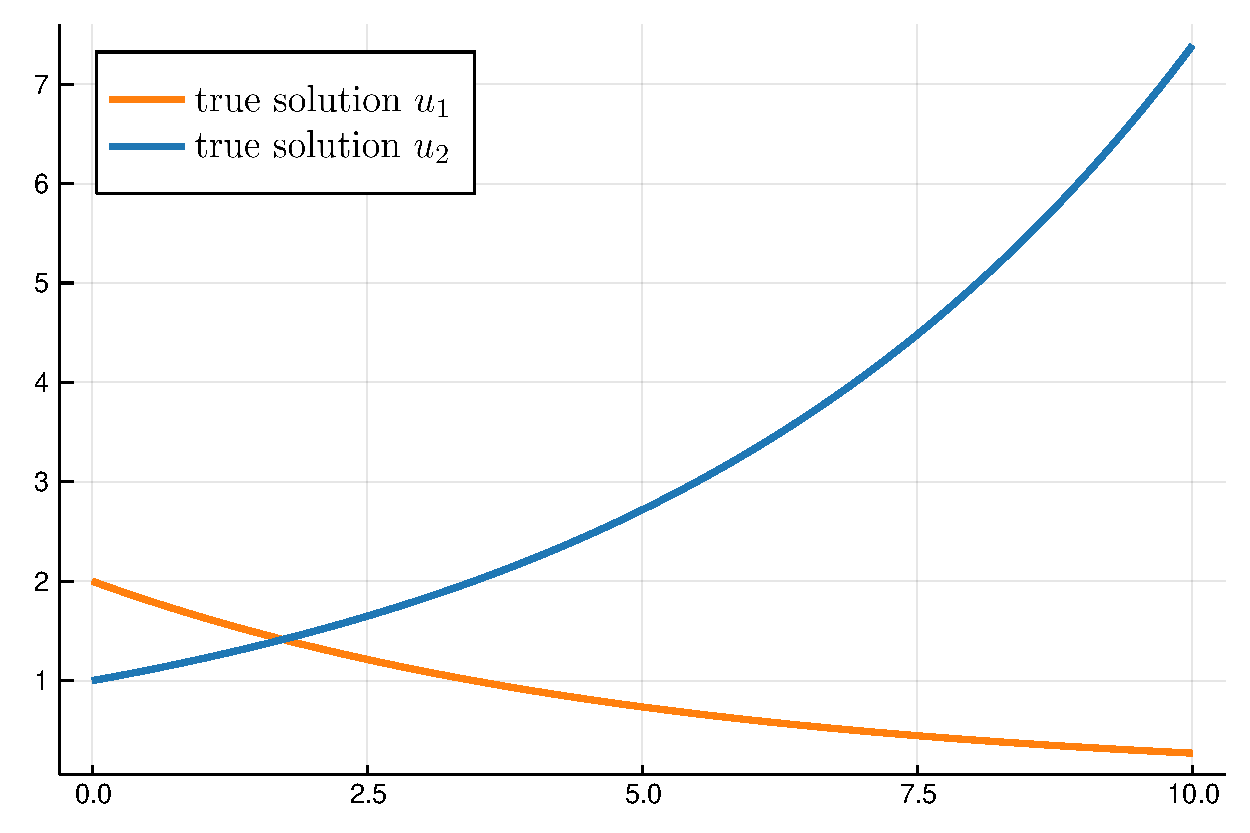
\includegraphics[width=\linewidth]{true_solution_2_2ps_linear.pdf}
		\scriptsize
		\begin{equation}\label{eq:ODE-systems-2ps-linear1}
		\begin{split}
		\frac{d}{dt}\begin{pmatrix} u_1 \\ u_2 \end{pmatrix}(t) &= \begin{pmatrix} -0.2 & 0 \\ 0 & 0.2 \end{pmatrix} \begin{pmatrix} u_1 \\ u_2 \end{pmatrix}(t); \\
		\begin{pmatrix} u_1 \\ u_2 \end{pmatrix}(0) &= \begin{pmatrix} 2 \\ 1 \end{pmatrix}
		\end{split}
		\end{equation}
		\normalsize
	\end{minipage}\begin{minipage}{.5\linewidth}
		\centering
		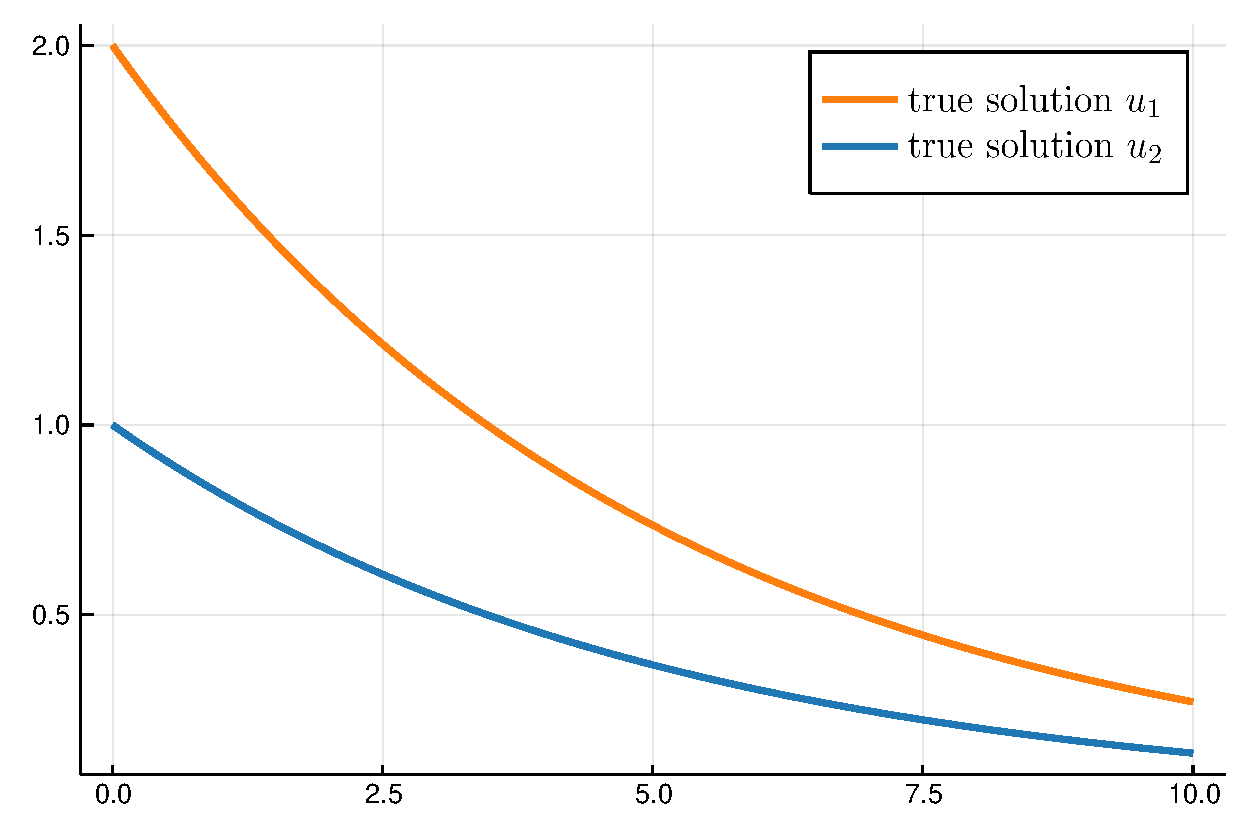
\includegraphics[width=\linewidth]{true_solution_1_2ps_linear.pdf}
		\scriptsize		
		\begin{equation}\label{eq:ODE-systems-2ps-linear2}
		\begin{split}
			\frac{d}{dt}\begin{pmatrix} u_1 \\ u_2 \end{pmatrix}(t) &= \begin{pmatrix} -0.2 & 0 \\ 0 & -0.2 \end{pmatrix} \begin{pmatrix} u_1 \\ u_2 \end{pmatrix}(t); \\
			\begin{pmatrix} u_1 \\ u_2 \end{pmatrix}(0) &= \begin{pmatrix} 2 \\ 1 \end{pmatrix}
		\end{split}
		\end{equation}
		\normalsize
	\end{minipage}
	\caption{True underlying development patterns characterised as solutions of two-dimensional linear ODE systems.}
	\label{fig:true_solution_linear_2ps}
\end{figure}

The data is simulated by drawing measurement points from these true trajectories with random noise as described in Algorithm~\ref{algo-simulation-time-dependent}. More precisely, I generate observations of $100$ individuals, $50$ from each of the two groups, and generate observations of $10$ variables by adding variable-specific and the individual-specific measurement errors to $5$ values from each of the two ODE solution components both at the initial time point $t_0 = 0$ and an individual-specific second time point $t_1^i$. In this first setting, I simulate a low level of noise and set $\sigma_{\mathrm{var}} = \sigma_{\mathrm{ind}} = 0.1$. Figure~\ref{fig:data_truesolution_linear2ps} visualises all simulated observations together with the true ODE solutions.
\begin{figure}
	\centering
	\begin{minipage}{.5\linewidth}
		\centering
		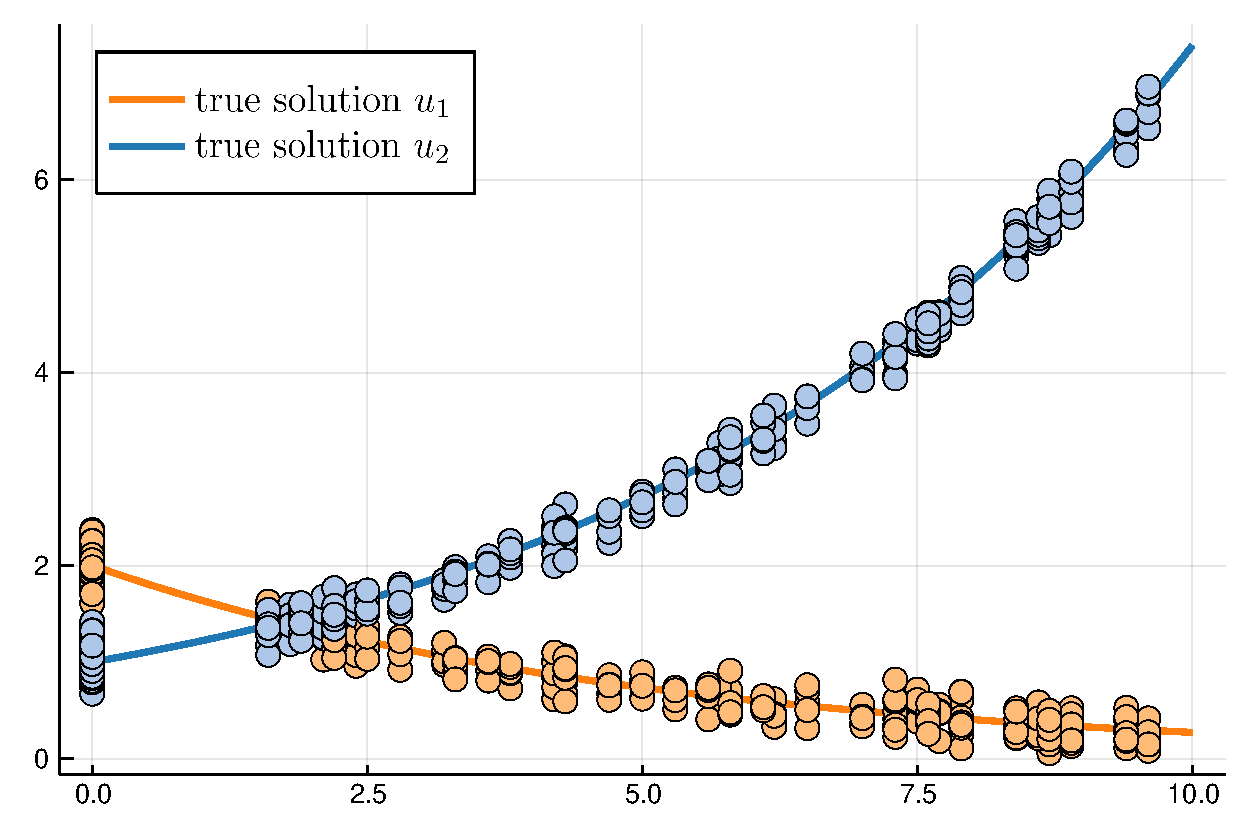
\includegraphics[width=\linewidth]{data_true_solution_2_2ps_linear.pdf}
	\end{minipage}\begin{minipage}{.5\linewidth}
		\centering
		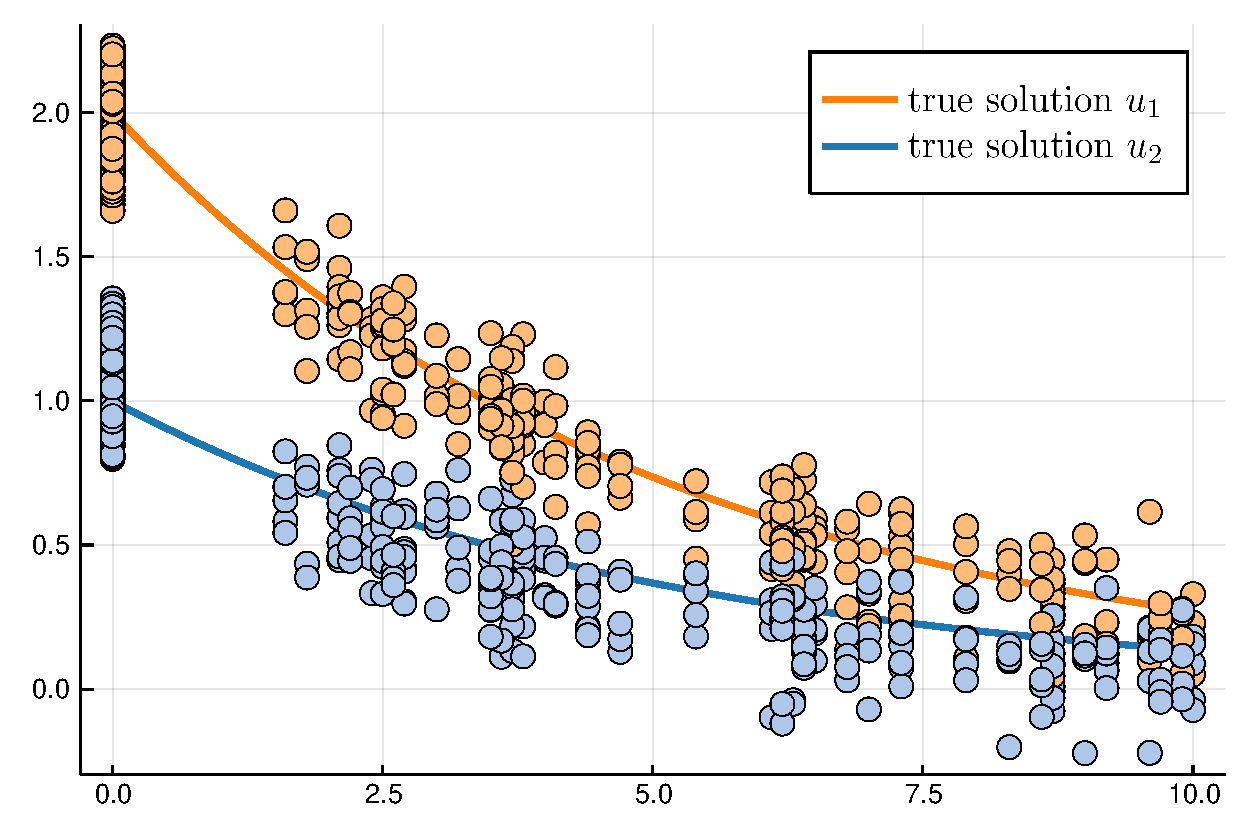
\includegraphics[width=\linewidth]{data_true_solution_1_2ps_linear.pdf}
	\end{minipage}
	\caption{Simulated observations of $100$ individuals ($50$ in each group) at $t_0$ and an individual-specific time point $t_1^i$.}
	\label{fig:data_truesolution_linear2ps}
\end{figure}
To illustrate the structure of each simulated individual's observations, Figure~\ref{fig:20example-ovservations_2ps_linear} exemplarily shows the observations of $20$ simulated study participants on an individual level. Each panel represents one individual, dots represent individual measurements and colors indicate different variables similar to Figure~\ref{fig:exemplary-data} in the introduction. 
\begin{figure}
	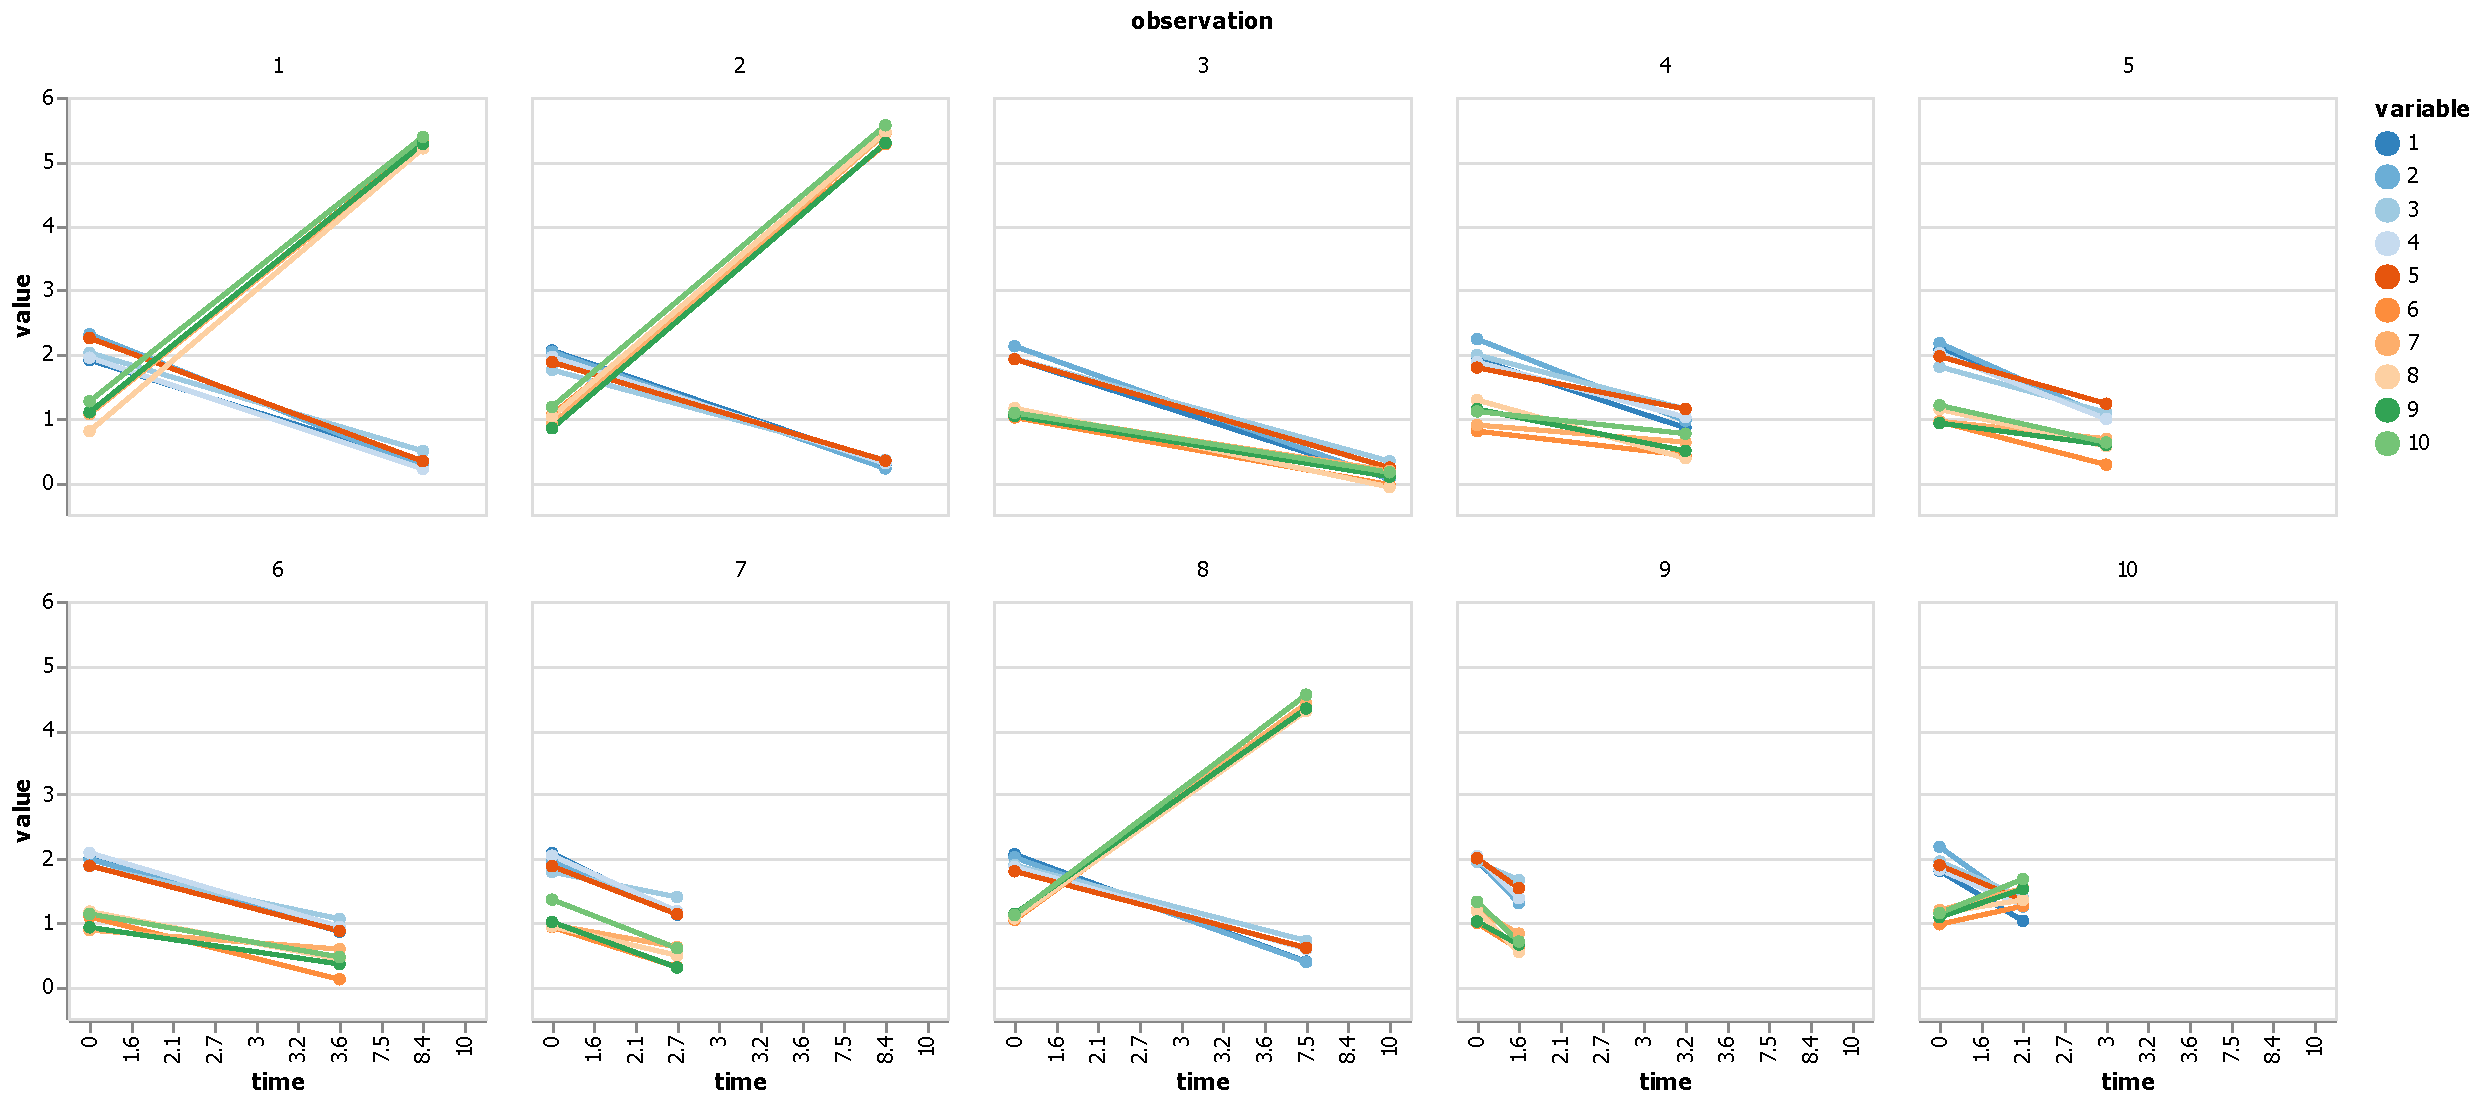
\includegraphics[width=\linewidth]{plot_of_10_example_observations_2ps_linear.pdf}
	\caption{Individual-level simulated data structure of $20$ individuals.}
	\label{fig:20example-ovservations_2ps_linear}
\end{figure}

\subsection{Comparison of different simulation scenarios of baseline variables}\label{sec:apps-linear2p-comparisonbaseline}

On the simulated data described in the previous section, the ODE-VAE model is trained as described in Chapter~\ref{chap:methods}, Section~\ref{sec:methods-ODE-VAEtraining}. Specifically, the ODE-net estimates the two non-zero parameters of each of the two ODE systems while the two off-diagonal entries are set to zero, i.e., no interaction is allowed between the components of the ODE solution. Thus, for each individual $i$ the initial value problem 
\begin{equation*}
\begin{split}
	\frac{d}{dt} \mu_i(t) &= \begin{pmatrix} \eta_{i,1} && 0 \\ 0 && \eta_{i,2}	\end{pmatrix} \begin{pmatrix} \mu_{i,1} \\ \mu_{i,2}	\end{pmatrix} (t); \\
	\mu_i(t_0) &= \mu_i\te
\end{split}
\end{equation*}
is solved in latent space at the individual's second measurement time point $t_i^1$ with ODE-net outputs $\eta_{i,1}, \eta_{i,2}$. 

As a first application, I compare the different simulations scenarios of baseline variables described in Algorithms~\ref{algo-simulation-baseline-trueODEparams} and \ref{algo-simulation-baseline-groupinfo}. For the first scenario with the true ODE parameters, I set $\sigma_{\mathrm{info}} = \sigma_{\mathrm{noise}} = 0.1$ and for the second scenario with the group membership, I set $\sigma_{\mathrm{info}} = \sigma_{\mathrm{noise}} = 0.5$, such that for both scenarios, the distributions of noise and the information overlap beyond one standard deviation. In each scenario, I simulate $10$ variables containing the respective baseline information, add $40$ noise variables and train the model for $35$ epochs with the ADAM SGD-optimiser (\cite{Kingma2015}) and a learning rate of $0.0005$. 

Figure~\ref{fig:apps_individual_comparison_tp_gi_2pslinear} depicts the fitted ODE solutions of two individuals both for a model trained with the true ODE parameters and one trained with only the group membership as baseline information. In both scenarios, the model recovers the general structure of the underlying patterns, recognising the distinct upward/downward trends of variables for the two individuals. 
It tends to overestimate the initial value of the first component of the solution and to underestimate it in the second component. For the training with the true ODE parameters, the overestimation of the first component initial value is more pronounced, whereas the underestimation in the second component is smaller than for training with only the group information. 
In both scenarios, the first dimension of the mean obtained directly from the VAE encoder before solving the ODE (blue dots) closely matches the first dimension of the smooth mean obtained as ODE solution (solid blue lines), whereas for the second component, in the second group, the means from the encoder for the second time point (orange dots) match the true ODE solution (dotted orange lines) more closely than the fitted ODE solutions. 
Thus, in general the training strategy 
of matching the means before and after solving the ODE -- to both find a latent representation modelling a smooth trajectory even before solving the ODE and to implicitly condition the ODE solution on the data from the second time point -- works, while there is some variation in whether the focus on matching the ODE solution or matching the data dominates. 
\begin{figure}
	\centering
	\begin{minipage}{\linewidth}
		\begin{minipage}{.5\textwidth}
			\centering				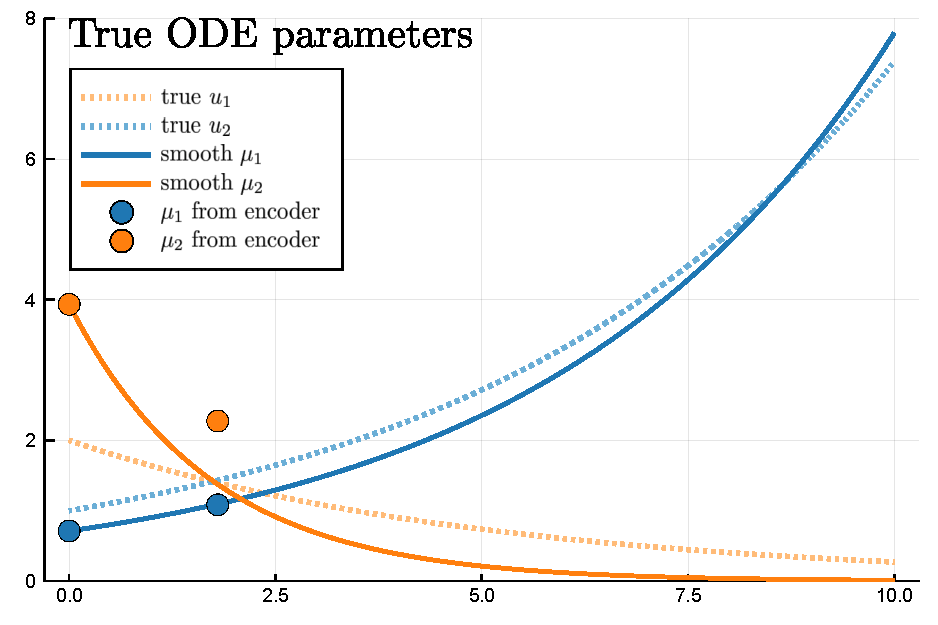
\includegraphics[width=\linewidth]{z_trajectory_plots_2ps_29_tp.pdf}
		\end{minipage}\begin{minipage}{.5\textwidth}
			\centering
			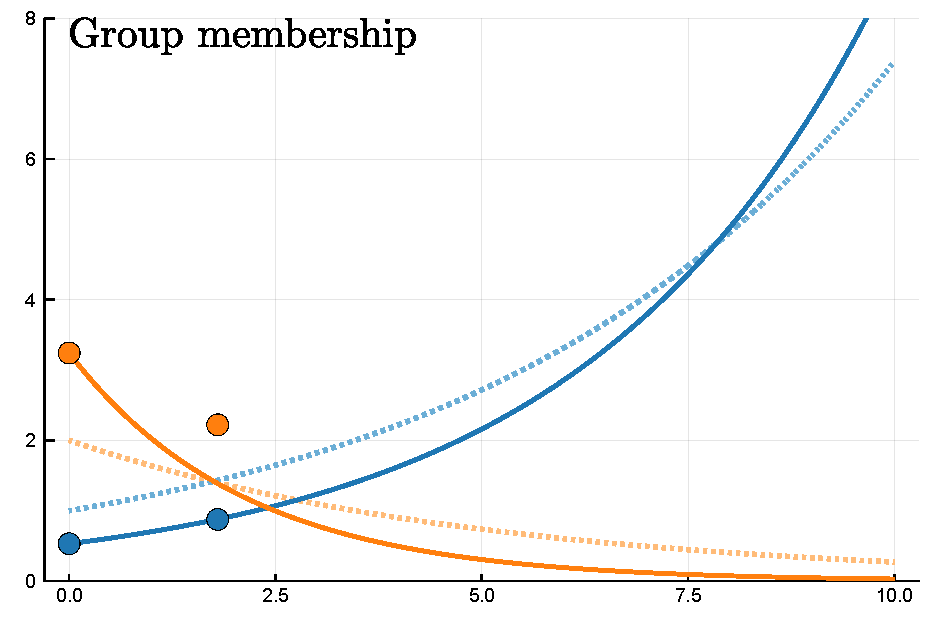
\includegraphics[width=\linewidth]{z_trajectory_plots_2ps_29_gi.pdf}
		\end{minipage}
	\end{minipage}
	\begin{minipage}{\linewidth}
		\begin{minipage}{.5\textwidth}
			\centering
			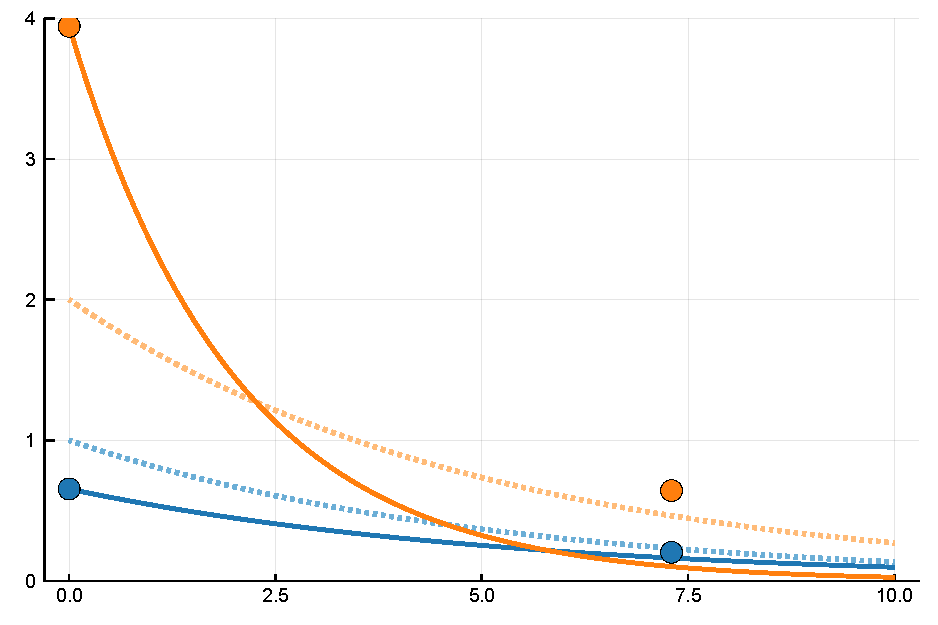
\includegraphics[width=\linewidth]{z_trajectory_plots_2ps_25_tp.pdf}
		\end{minipage}\begin{minipage}{.5\textwidth}
			\centering
			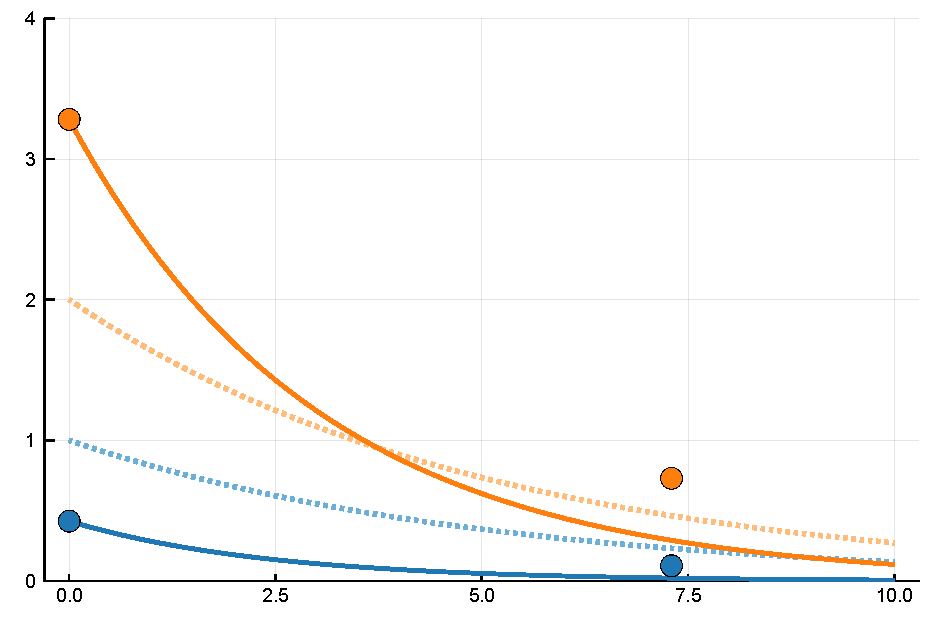
\includegraphics[width=\linewidth]{z_trajectory_plots_2ps_25_gi.pdf}
		\end{minipage}
	\end{minipage}
\caption{Comparison of fitted ODE solutions of one individual from each group for both scenarios of simulated baseline variables.}
\label{fig:apps_individual_comparison_tp_gi_2pslinear}
\end{figure}

To get a broader overview, the distributions of ODE solutions are compared across the whole dataset. In Figure~\ref{fig:apps_allinds_comparison_tp_gi_2pslinear}, the fitted ODE solutions and encoder means from all individuals of one group are overlayed, and again both groups of underlying development patterns and both scenarios of baseline variables are compared. 

As expected, the results from training with only the group membership as baseline information, representing the more difficult scenario, display a higher variability between individual ODE solutions in both groups. 
In this setting, the model also has greater difficulty matching the upward development in the first group of individuals with the posterior mean before solving the ODE (blue dots). While this trend is underestimated especially for later timepoints ($t>6$) also with the true ODE parameters as baseline information, this becomes more pronounced for training with only the group membership. For both groups and both training scenarios, it seems to be difficult to capture the exponential growth or decay in the latent representation mean before solving the ODE, as can be seen from the blue dots in the panels in the first row and the orange dots in the second row forming a linear rather than an exponential trend. Only the exponential decay of the first ODE component for the first group of individuals is captured in the encoder means (orange dots in the first row).

\begin{figure}
	\centering
	\begin{minipage}{\linewidth}
		\begin{minipage}{.5\textwidth}
			\centering				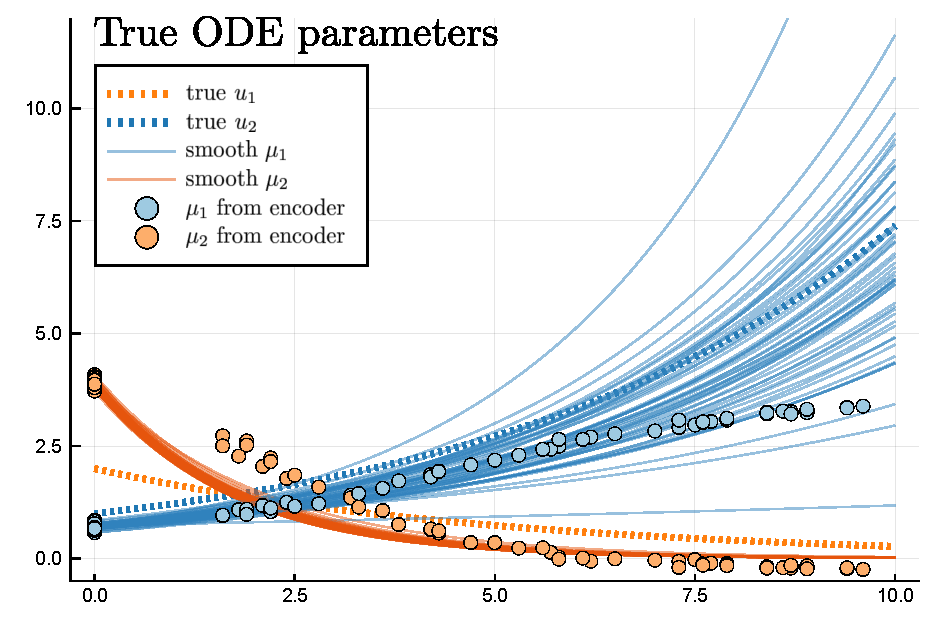
\includegraphics[width=\linewidth]{all_inds_overlaid_group2_tp_2ps_linear.pdf}
		\end{minipage}\begin{minipage}{.5\textwidth}
			\centering
			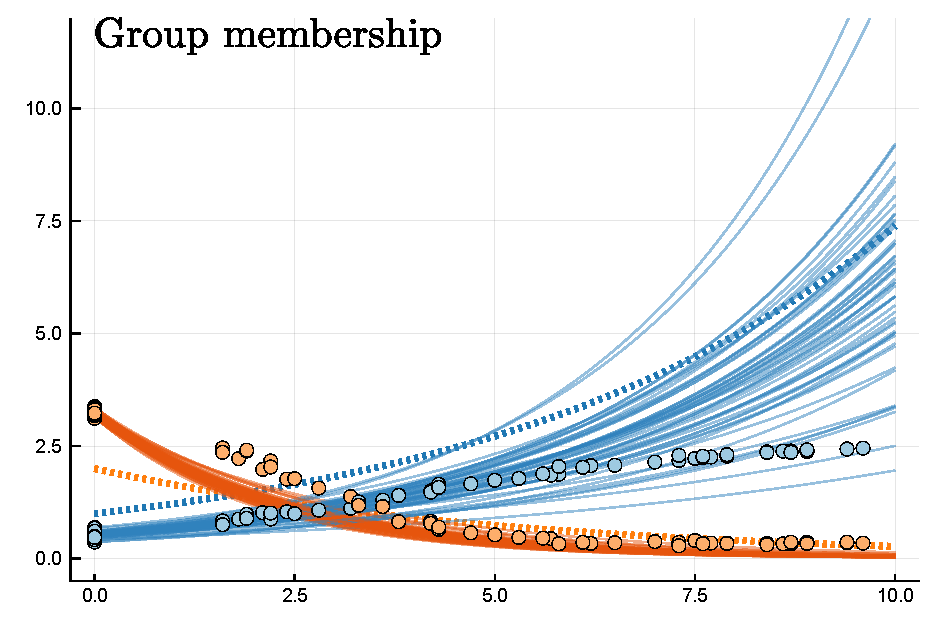
\includegraphics[width=\linewidth]{all_inds_overlaid_group2_gi_2ps_linear.pdf}
		\end{minipage}
	\end{minipage}
	\begin{minipage}{\linewidth}
		\begin{minipage}{.5\textwidth}
			\centering
			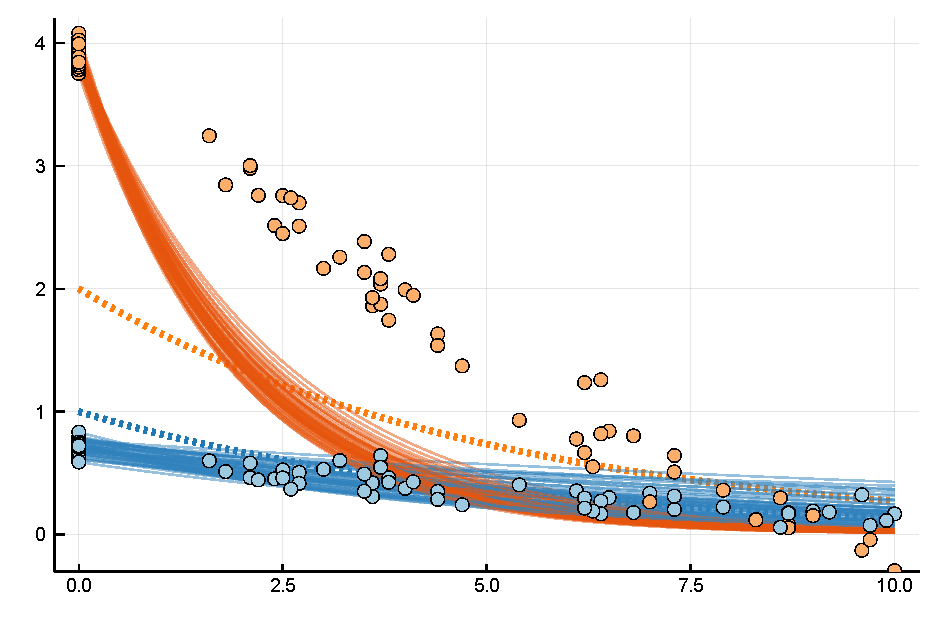
\includegraphics[width=\linewidth]{all_inds_overlaid_group1_tp_2ps_linear.pdf}
		\end{minipage}\begin{minipage}{.5\textwidth}
			\centering
			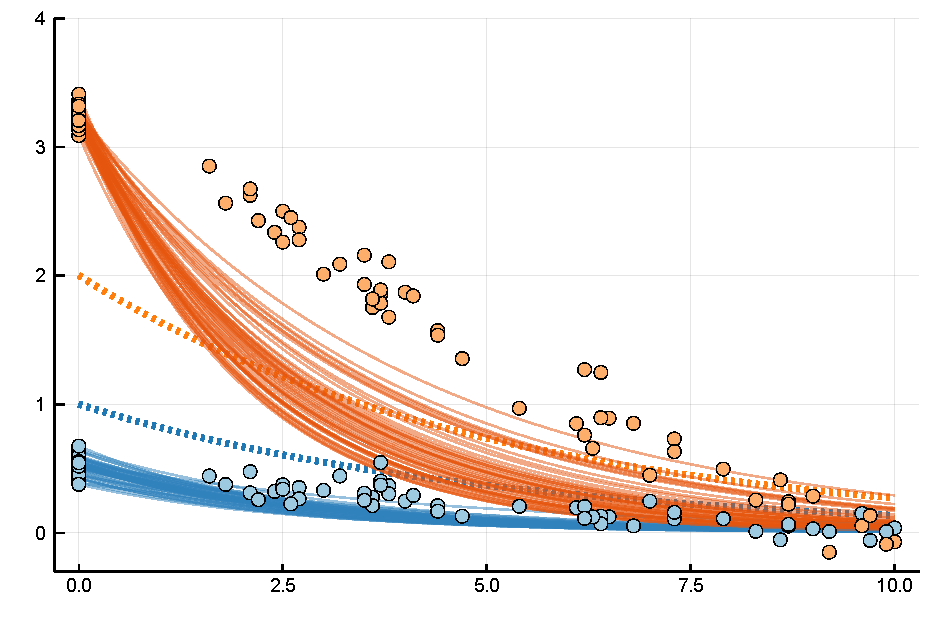
\includegraphics[width=\linewidth]{all_inds_overlaid_group1_gi_2ps_linear.pdf}
		\end{minipage}
	\end{minipage}
	\caption{Comparison of fitted ODE solutions of all individual from each group for both scenarios of simulated baseline variables.}
	\label{fig:apps_allinds_comparison_tp_gi_2pslinear}
\end{figure}

\subsection{Comparison of different noise levels in the simulated data}\label{sec:apps-linear2p-comparisonnoise}

To investigate how different levels of noise in the time-dependent variables affect the training of the model, I compare the scenario described in Section~\ref{sec:apps-linear2p-inputdata} to a scenario with the same number of observations from the same underlying ODE solutions, but a higher level of random noise. Specifically, I set $\sigma_{\mathrm{var}} = 0.5$ and $\sigma_{\mathrm{ind}} = 1$. As in Figures~\ref{fig:data_truesolution_linear2ps} and \ref{fig:20example-ovservations_2ps_linear} for the setting with a low level of noise, Figure~\ref{fig:data_truesolution_linear2ps_morenoise} visualises all simulated measurements together with the true ODE solutions while the individual-level structure of $20$ simulated individuals is exemplarily illustrated in Figure~\ref{fig:20example-ovservations_2ps_linear_morenoise}.
\begin{figure}
	\centering
	\begin{minipage}{.5\linewidth}
		\centering
		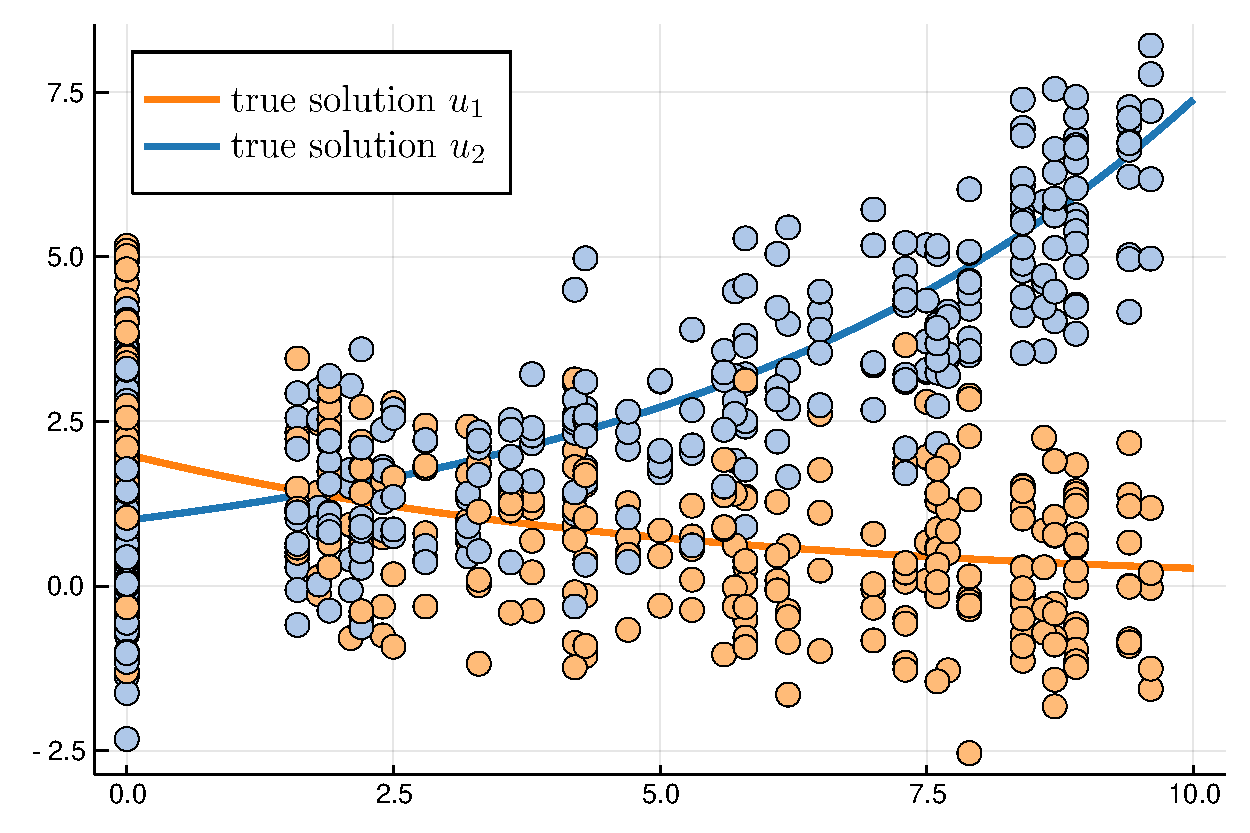
\includegraphics[width=\linewidth]{data_true_solution_2_2ps_linear_morenoise.pdf}
	\end{minipage}\begin{minipage}{.5\linewidth}
		\centering
		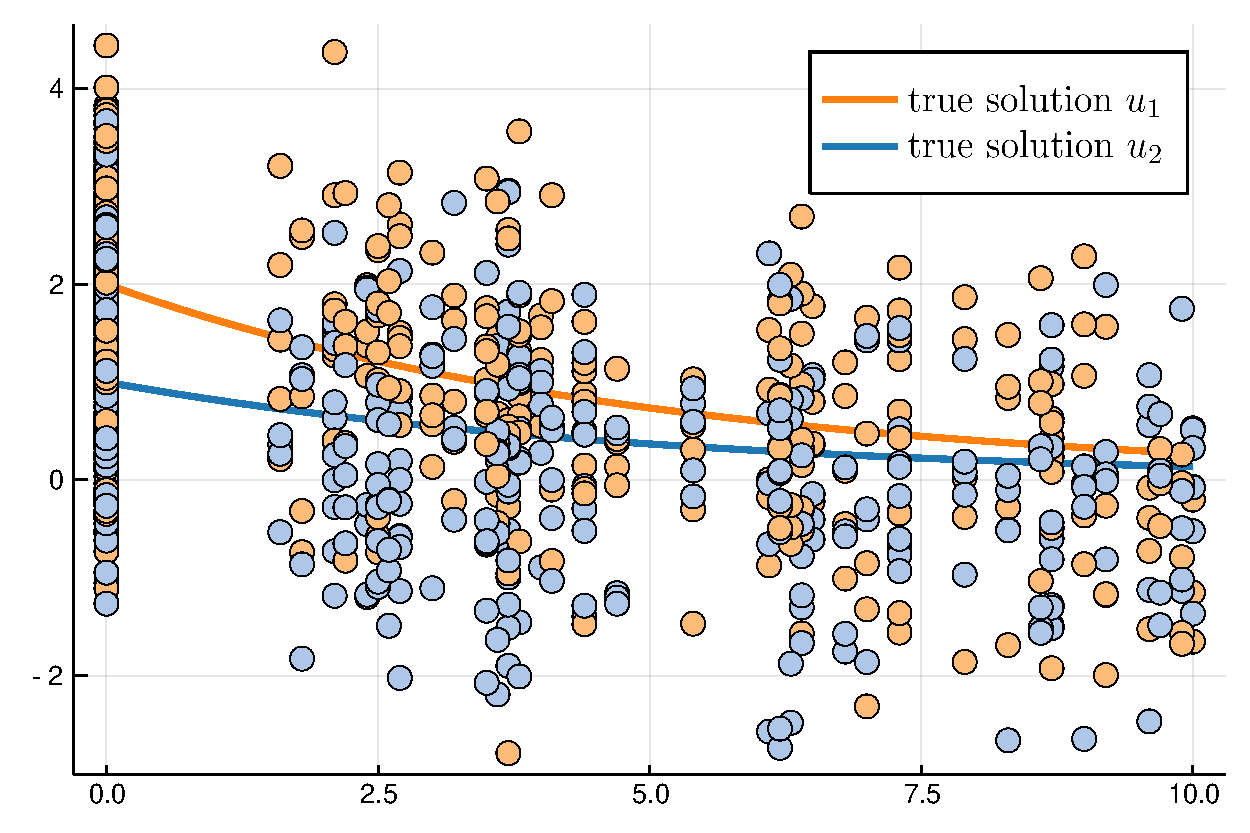
\includegraphics[width=\linewidth]{data_true_solution_1_2ps_linear_morenoise.pdf}
	\end{minipage}
	\caption{Simulated observations of $100$ individuals ($50$ in each group) at $t_0$ and an individual-specific time point $t_1^i$.}
	\label{fig:data_truesolution_linear2ps_morenoise}
\end{figure}
\begin{figure}
	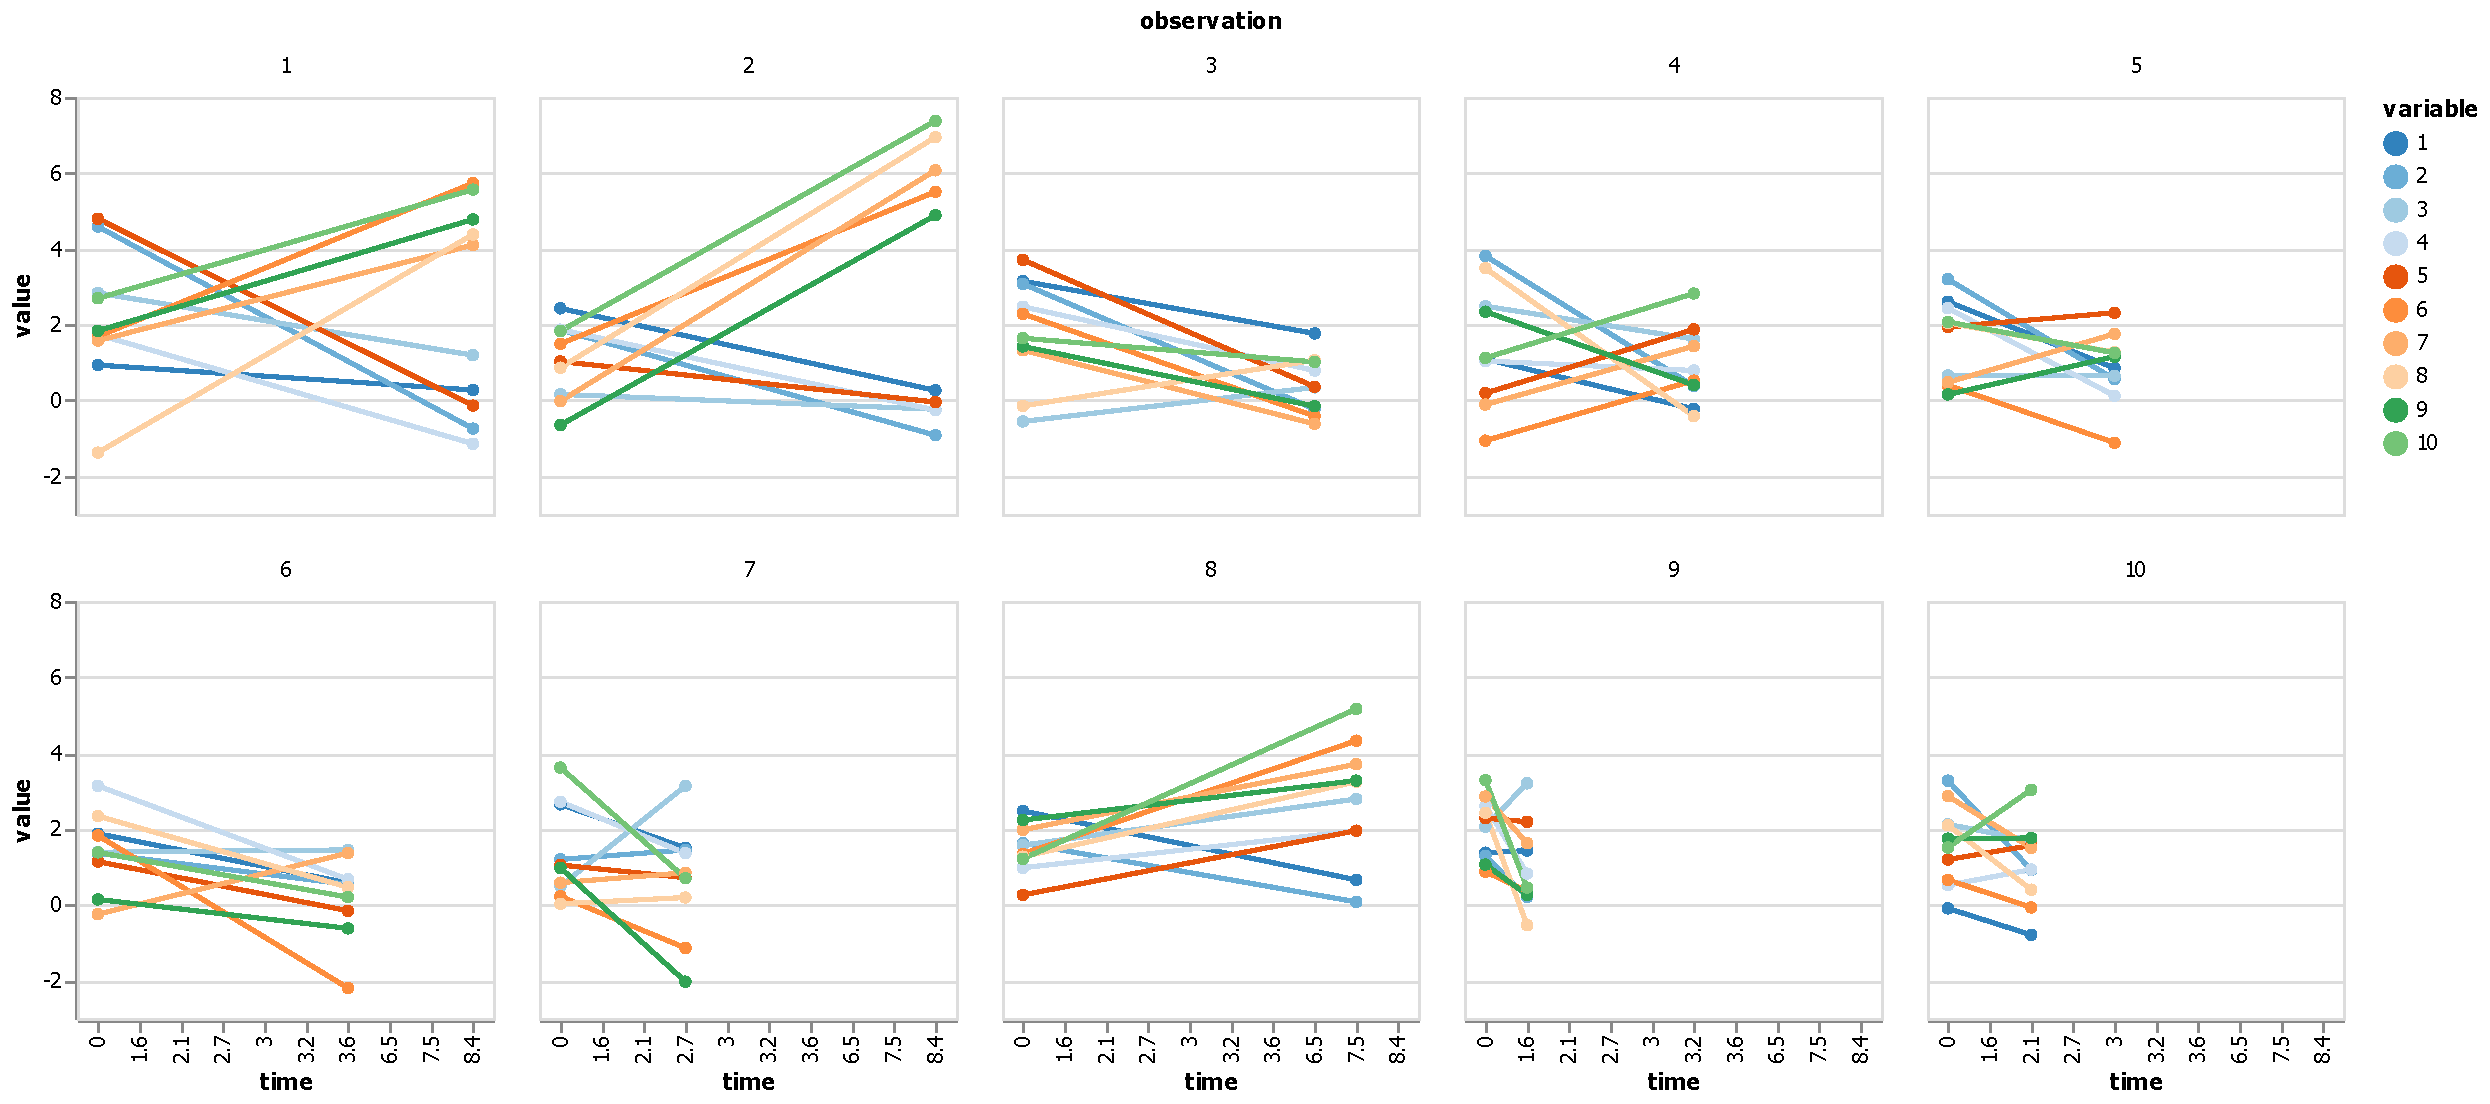
\includegraphics[width=\linewidth]{plot_of_10_example_observations_2ps_linear_morenoise.pdf}
	\caption{Individual-level simulated data structure of $20$ individuals.}
	\label{fig:20example-ovservations_2ps_linear_morenoise}
\end{figure}
For this setting of noisier observations of the true trajectories, I simulate the two versions of baseline variables exactly as in the previous Section~\ref{sec:apps-linear2p-comparisonbaseline} and train the model for $35$ epochs with the ADAM-optimiser and a learning rate of $0.001$.
Figure~\ref{fig:apps_allinds_comparison_morelessnoise_bothgroups_linear} shows a comparison of the results with those from the less noisy setting.
% depicted in Figure~\ref{fig:apps_allinds_comparison_tp_gi_2pslinear}.  
\begin{figure}
	\centering
	\begin{minipage}{\linewidth}
	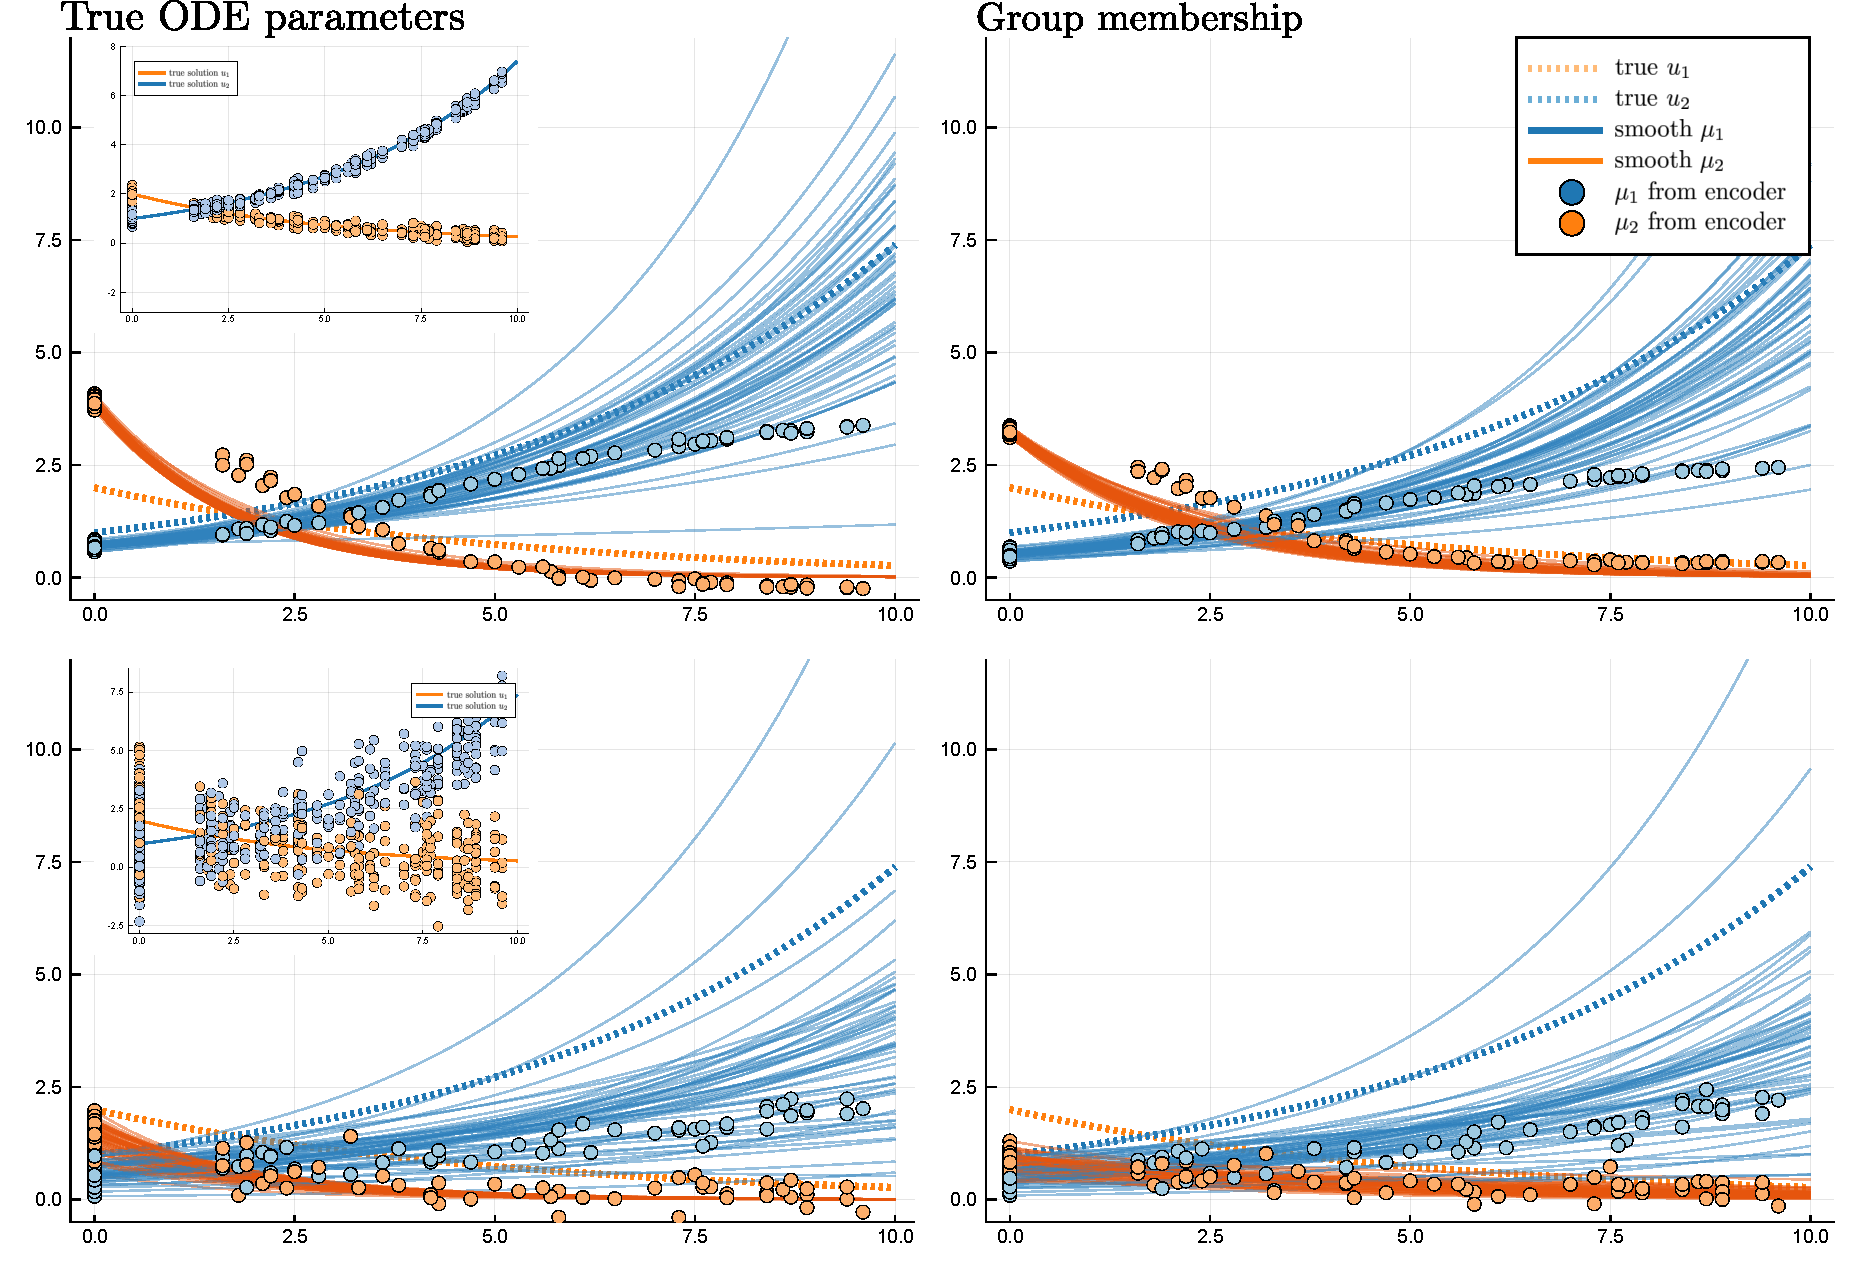
\includegraphics[width=\linewidth]{comparison_more_less_noise_linear_2ps_group2.pdf}
	\end{minipage}
	\begin{minipage}{\linewidth}
		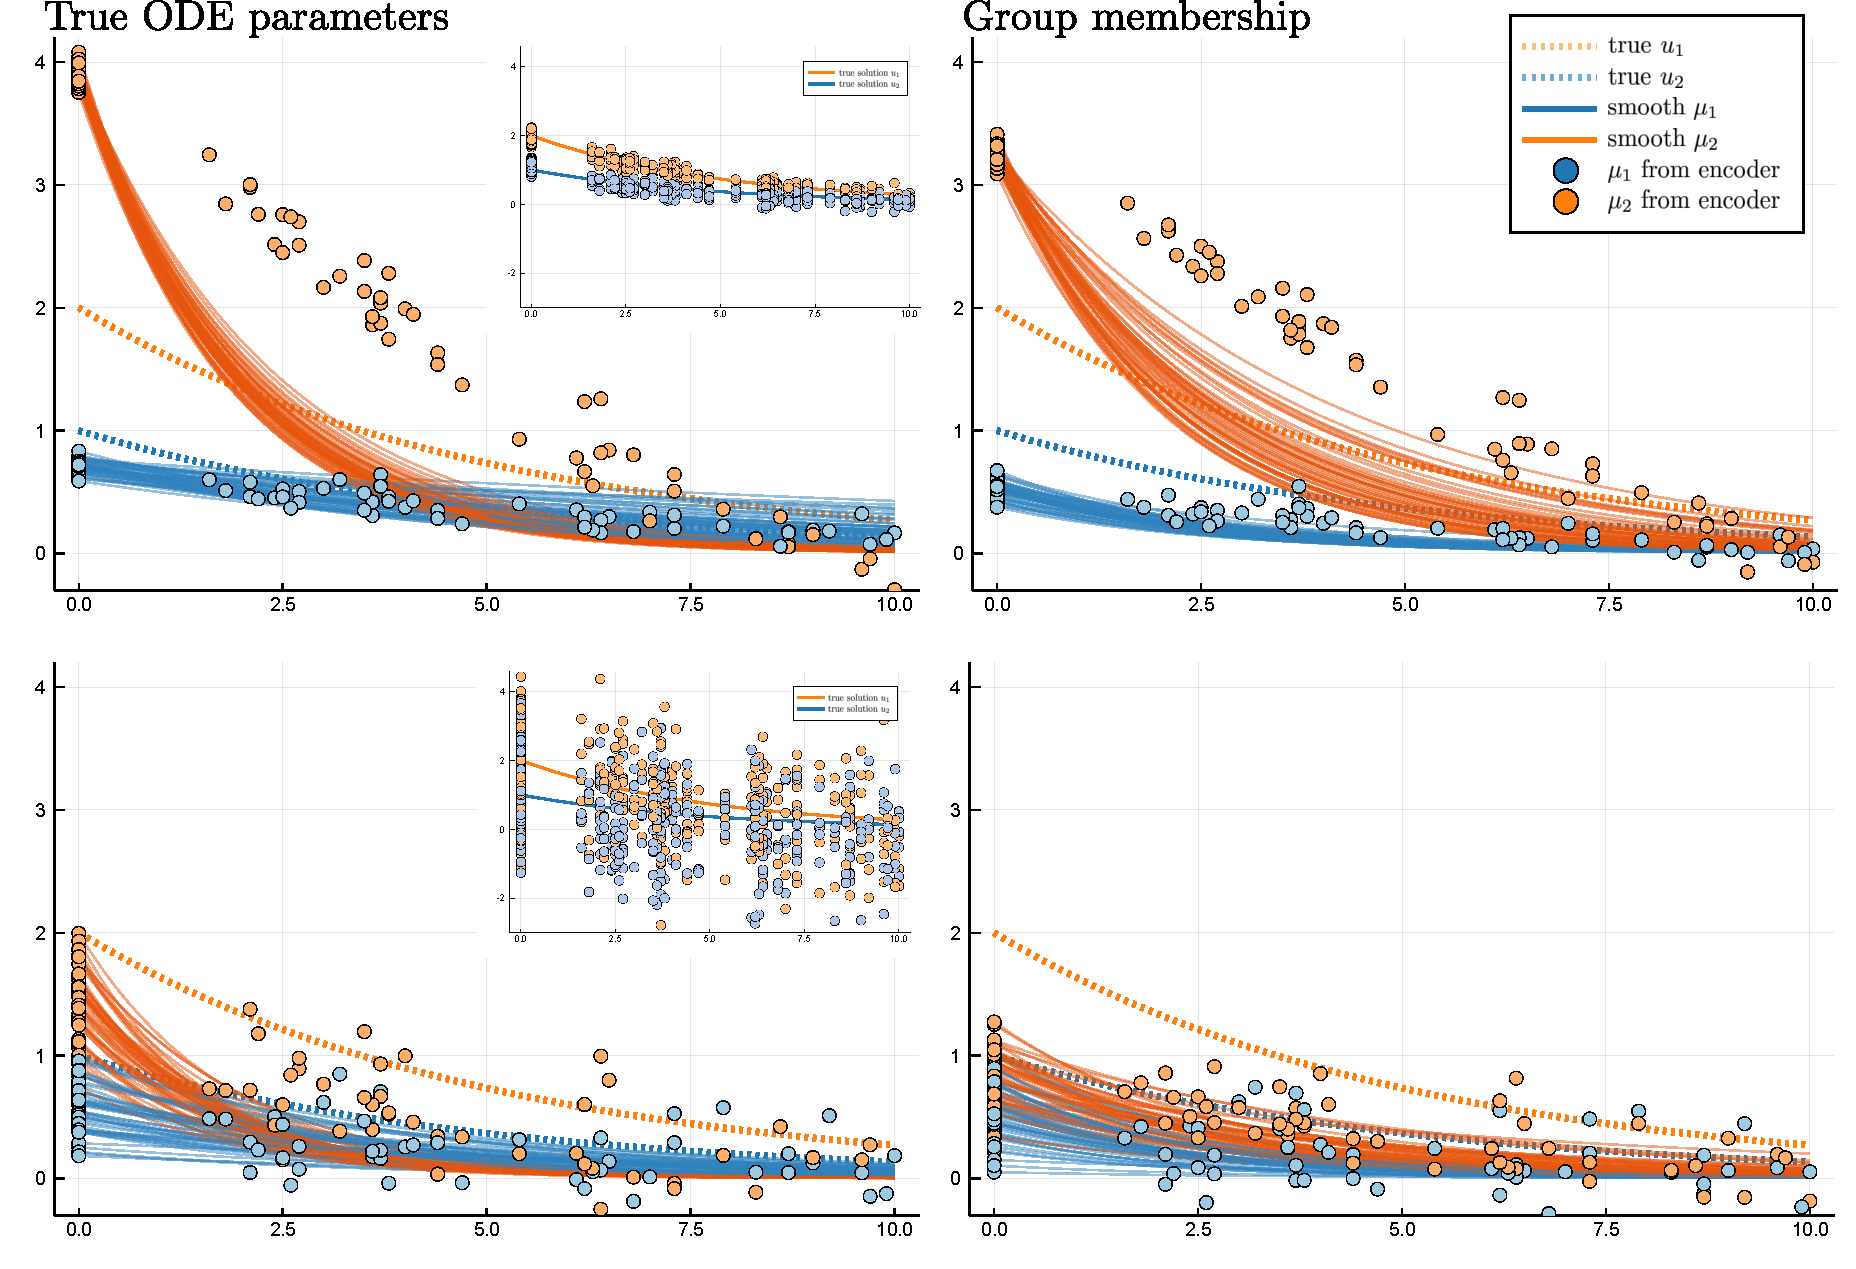
\includegraphics[width=\linewidth]{comparison_more_less_noise_linear_2ps_group1.pdf}
	\end{minipage}
	\caption{Comparison of fitted ODE solutions of all individual from both groups for both scenarios of simulated baseline variables and two different noise levels.}
	\label{fig:apps_allinds_comparison_morelessnoise_bothgroups_linear}
\end{figure}

First, we can observe that the noisier data setting results in higher variability between fitted ODE solutions (solid lines) as well as the means obtained directly from the encoder (dots) of different individuals. Especially for the second group of individuals (last row), the two components of the mean both from the encoder and as ODE solution are not as distinctly separated. This reflects the setting in the input data: Here, also, the higher noise level results in a substantial overlay of the simulated measurements of both components (see Figure~\ref{fig:data_truesolution_linear2ps_morenoise} and the small figure in the last row of Figure~\ref{fig:apps_allinds_comparison_morelessnoise_bothgroups_linear}). When trained with only the group membership as baseline information, the variability further increases as before, as does the underestimation of the upward trend in the first group of individuals. In the noisier setting, also the downward trend of the first ODE solution component (dotted orange lines) is underestimated in both groups of individuals. 
This is potentially due to the variational posterior being more heavily influenced by the regularising $\mathcal{N}(0,I)$-prior when it gets a weaker input from the data. 

Generally, as the data becomes noisier and the baseline variables become less informative, the latent representations get blurrier, the variability between individuals increases and the two components become less discintly separated, as becomes particularly apparent at the initial value. Nonetheless, despite the substantial level of noise in the data, the model still recovers the general trends and the individual-specific structure of the development patterns. 

\subsection{Training variability}\label{sec:apps-linear2ps-trainingvariability}

As the training objective (\ref{finalELBO}) of the ODE-VAE model represents a non-convex function and hence does not have a unique minimum, the SGD iterative optimisation procedure only approximates a local optimum that depends on the starting point of the algorithm, i.e., the random initialisation of the model weights and biases. To assess the stability with respect to the initialisation, I compare the results across several training runs.

For this application, I employ a moderate level of noise in the time-dependent variables in between the more extreme scenarios compared in the previous Section~\ref{sec:apps-linear2p-comparisonnoise} and set $\sigma_{\mathrm{var}} = 0.1$ and $\sigma_{\mathrm{ind}} = 0.5$. The resulting simulated measurements of the true trajectories are depicted in Figure~\ref{fig:data_truesolution_linear2ps_trainingvariability}.
\begin{figure}
	\centering
	\begin{minipage}{.5\linewidth}
		\centering
		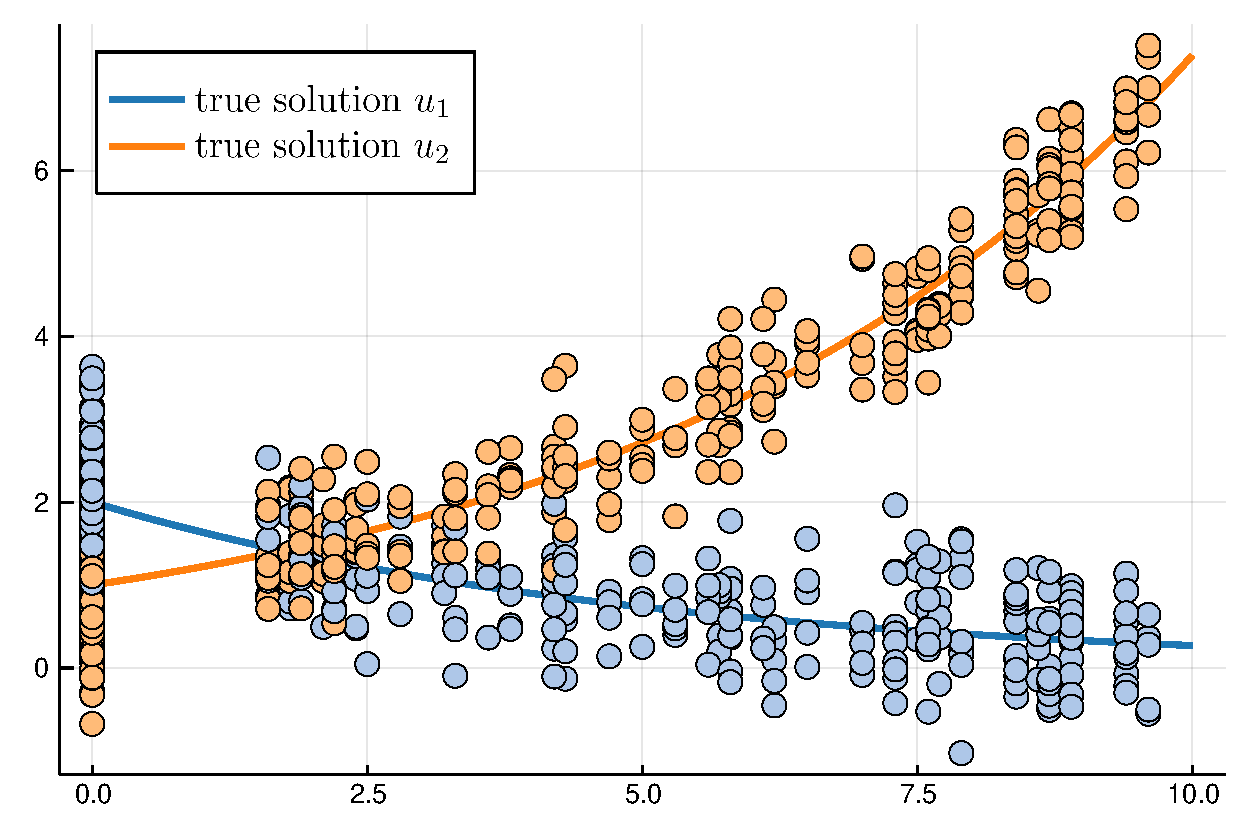
\includegraphics[width=\linewidth]{data_true_solution_2_trainingvariability.pdf}
	\end{minipage}\begin{minipage}{.5\linewidth}
		\centering
		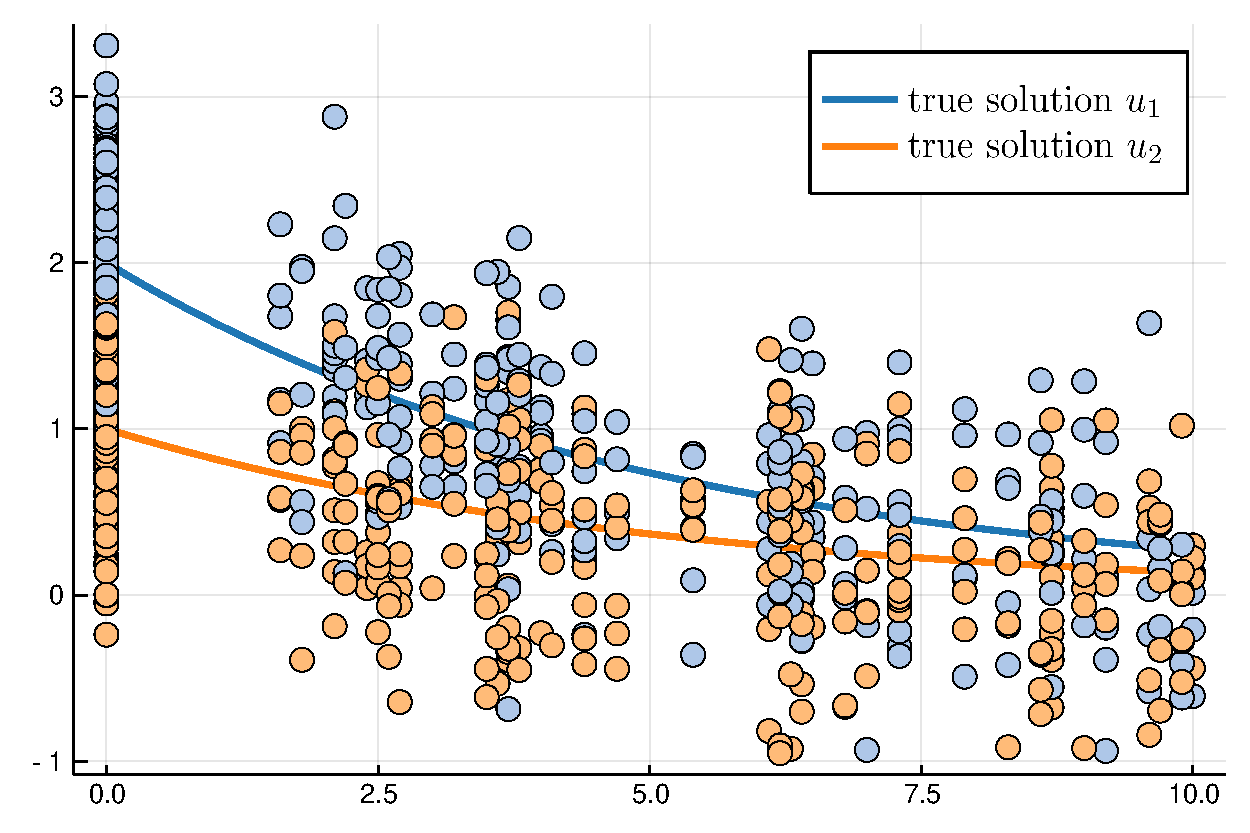
\includegraphics[width=\linewidth]{data_true_solution_1_trainingvariability.pdf}
	\end{minipage}
	\caption{Simulated observations of $100$ individuals ($50$ in each group) at $t_0$ and an individual-specific time point $t_1^i$.}
	\label{fig:data_truesolution_linear2ps_trainingvariability}
\end{figure}

I employ the same two scenarios of simulated baseline variables as before and for each scenario conduct $10$ training runs of the model with different random weight initialisations. In each run, I train the model for $35$ epochs with the ADAM-optimiser and a learning rate of $0.001$. The results are shown in Figure~\ref{fig:apps_training_variability_tp_1} (true ODE parameters as baseline information) and Figure~\ref{fig:apps_training_variability_gi_1} (group membership).
\begin{figure}
	\centering
	\includegraphics[width=\linewidth]{training_variability_bothgroups_trueODEparams_1.pdf}
	\caption{Results of $10$ training runs for model trained with true ODE parameters as baseline information. Each row depicts two training runs and for each run, the two groups of individuals are shown in separate panels.}
	\label{fig:apps_training_variability_tp_1}
\end{figure}

\begin{figure}
	\centering
	\includegraphics[width=\linewidth]{training_variability_bothgroups_groupinfo_1.pdf}
	\caption{Results of $10$ training runs for model trained with group membership as baseline information.}
	\label{fig:apps_training_variability_gi_1}
\end{figure}

Note that the model quite frequently flips one or both components of the initial condition along the $x$-axis. However, the model then also reverses the trend shown by the true trajectories when it flips them to negative values, such that the sign of the corresponding ODE parameter remains the same (a positive parameter in the system defines an upward trend for a positive value of the initial condition and a downward trend for a negative value). The downward trends of the true solution turn into upward trends of the fitted solution when the model flips the initial condition, and vice versa. 
The model thus still infers the distinct group-specific development patterns and assigns to them the correct parameters of the ODE system, it merely embeds the data in a latent representation that flips the signs in one or both dimensions. The neural network architecture defining the model encoder and decoder grants the model freedom to structure its latent representation so that it can potentially flip the signs of the data values in the process of embedding them in latent space and flip them back again in the decoder, and does not enforce or even encourage a latent representation that keeps the signs of the original ODE solution. 
Additionally, the model freedom in structuring the latent space involves the possibility to rescale the input values, such that the entire system is captured in, e.g., a downscaled version. Potentially, this phenomenon may also account for the downscaled representation compared to the original true ODE solutions that we observed in some of the previous applications. 

Regularly, the model also swaps the dimensions, as can be seen from the training runs that appear to have an inverted colour coding: E.g., in the training run depicted in the two right panels in the second row, the orange fitted ODE solutions belonging to the first latent mean component $\mu_1$ match the second component of the ground truth-ODE solution $u_2$ shown in blue and vice versa. This phenomenon can be explained by the fact that the underlying system is symmetric in the two variables and again, the model structure allows it to fit the first five variables of each observation drawn from the first component $u_1$ of the true solution with the second component $\mu_2$ of its latent representation and vice versa. 

In all but one run (the two right panels in the third row in Figures~\ref{fig:apps_training_variability_tp_1} and \ref{fig:apps_training_variability_gi_1}), the model correctly identifies the distinct underlying development patterns in the two groups. 
This run remained the only one where the general structure was not captured by the model, also when I ran $10$ more runs with different initialisations (results not shown). 
The variability across the dataset differs and is generally higher in the means obtained directly from the encoder. Often, the variability in the second group of individuals appears higher, but this is mostly related to the different scale of the $y$-axis in the two groups. Overall, the observations made in Section~\ref{sec:apps-linear2p-comparisonbaseline} apply also to the majority of training runs depicted in Figures~\ref{fig:apps_training_variability_tp_1} and \ref{fig:apps_training_variability_gi_1}, suggesting that while the ODE-VAE model sometimes is subject to substantial variability in the fitted ODE solutions, it is generally capable of stably inferring distinctly parameterised underlying ODE systems.

\section{Non-linear ODE system with two unknown parameters}\label{sec:apps-nonlinear2p}

\subsection{Structure of input data}\label{sec:apps-nonlinear-inputdata}
In the following section, the model is applied on data from a non-linear ODE system. Specifically, I define two distinctly parameterised Lotka-Volterra systems. This two-dimensional non-linear system is used in ecology to describe the dynamics of the interaction of two populations generally denoted the predator and the prey species (\cite[p.~209]{Teschl2012}). The pair of equations is governed by four parameters and has the following form: 
\begin{equation}\label{eq:general-lotka-volterra-system}
	\begin{split}
			\frac{d}{dt} u_1(t) &= \alpha u_1(t) - \beta u_1(t)u_2(t), \\
			\frac{d}{dt} u_2(t) &= \delta u_1(t)u_2(t) - \gamma u_2(t)
	\end{split}
\end{equation}
In the predator-prey model, the first component $u_1$ describes the dynamics of the prey species and the second component $u_2$ describes that of the predator species. The model then assumes that the growth rate of the prey is $\alpha$, if there are no predators present, and that in the presence of predators, the growth rate is reduced proportional to the number of predators, i.e., $\beta$ can be understood as predation rate or meeting rate of prey and predator. Similarly, without prey, i.e., without food supply, the model assumes the number of predators to decay at rate $-\gamma$, and to increase, if there is prey,  proportional to the amount of prey, such that $\delta$ describes the growth rate of the predator in the presence of prey. 

Unlike the linear system employed in the previous Section~\ref{sec:apps-linear2p}, the periodic solutions of the Lotka-Volterra system cannot be calculated analytically in closed form, which means that the solution has to be approximated numerically. 
For more details on the properties of Lotka-Volterra systems, see \cite[pp.~209-215]{Teschl2012}. 

As for the linear system in Section~\ref{sec:apps-linear2p}, I simulate data from two different underlying development patterns given as solutions of the two distinctly parameterised Lotka-Volterra ODE systems defined in Equations (\ref{eq:ODEsystem-nonlinear-1}) and (\ref{eq:ODEsystem-nonlinear-2}) and visualised in Figure~\ref{fig:true_solution_lv}.

\begin{figure}
	\centering
	\begin{minipage}{.5\linewidth}
		\centering
		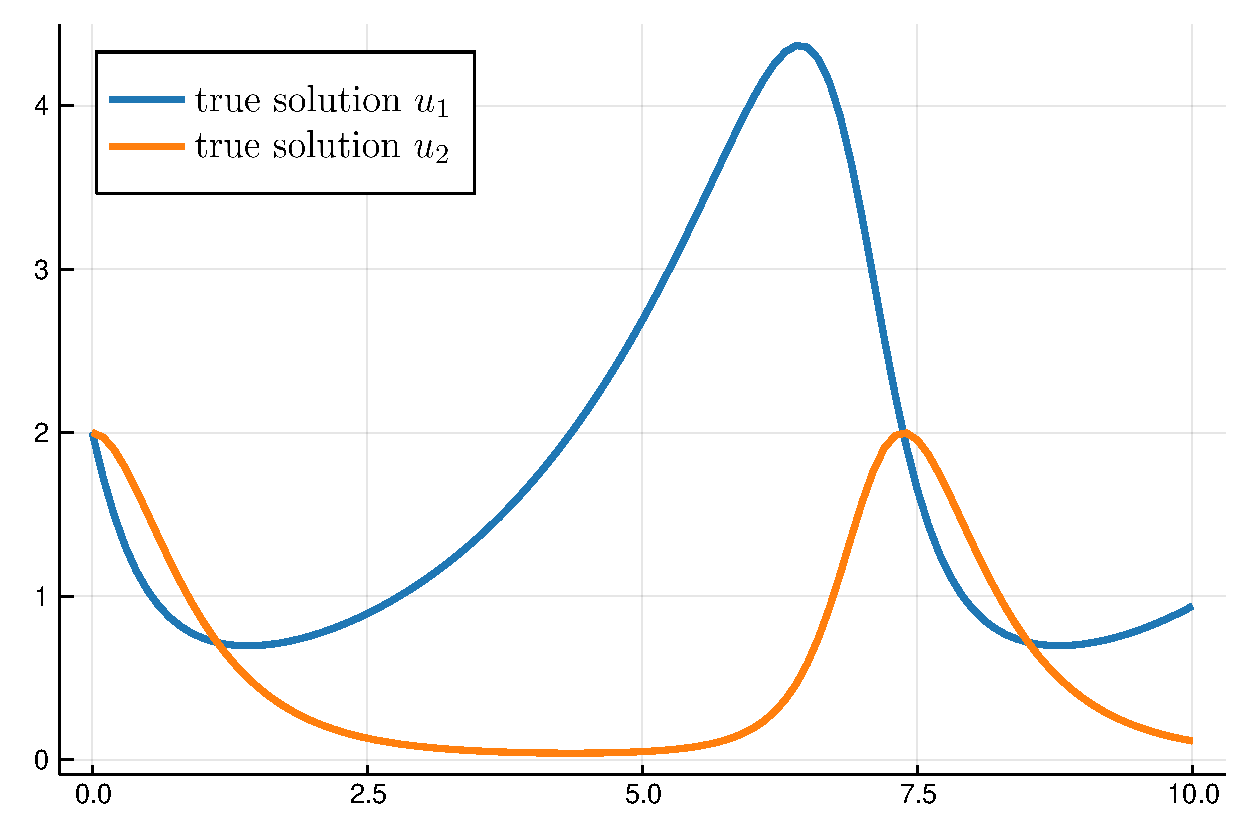
\includegraphics[width=\linewidth]{true_solution_2_lv.pdf}
		\begin{equation}\label{eq:ODEsystem-nonlinear-1}
		\begin{split}
				\frac{d}{dt}u_1(t) &= 0.5 u_1(t) - u_1(t) u_2(t), \\
				\frac{d}{dt}u_2(t) &= u_1(t) u_2(t) - 2 u_1(t); \\
				u_1(0) &= 2, \\ 
				u_2(0) &= 2
		\end{split}
		\end{equation}
		%\normalsize
	\end{minipage}\begin{minipage}{.5\linewidth}
		\centering
		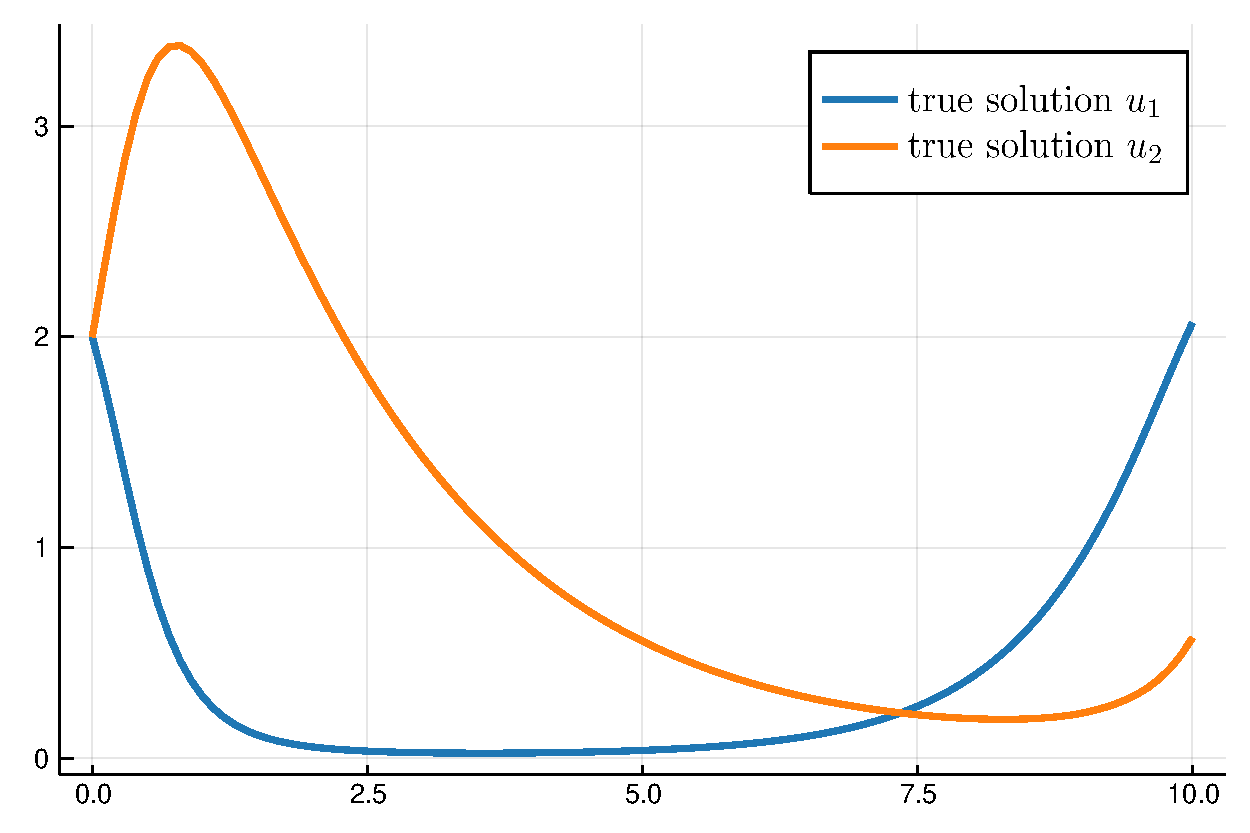
\includegraphics[width=\linewidth]{true_solution_1_lv.pdf}
		\begin{equation}\label{eq:ODEsystem-nonlinear-2}
		\begin{split}
				\frac{d}{dt}u_1(t) &= u_1(t) - u_1(t) u_2(t), \\
				\frac{d}{dt}u_2(t) &= u_1(t) u_2(t) - 0.5 u_1(t); \\
				u_1(0) &= 2, \\ 
				u_2(0) &= 2 
		\end{split}
		\end{equation}
		%\normalsize
	\end{minipage}
	\caption{True underlying development patterns characterised as solutions of two-dimensional Lotka-Volterra ODE systems.}
	\label{fig:true_solution_lv}
\end{figure}

As described in Algorithm~\ref{algo-simulation-time-dependent}, observations are simulated by adding random noise to values from these true trajectories. 
To account for the higher complexity of the true system, observations of $200$ individuals are generated in this application, such that the randomly drawn second measurement time points more densely cover the entire trajectory. Thus, the model gets observations from all different sections of the true underlying patterns (e.g., observations from the peak at the beginning of the time interval in the second ODE component of the second system, and the upward trend at the end of the time interval). 

Consequently, I generate observations of $100$ individuals in each of the two groups, and again generate observations of $10$ variables by adding variable-specific and the individual-specific measurement errors to $5$ values from each of the two ODE solution components both at the initial time point $t_0 = 0$ and an individual-specific second time point $t_1^i$. 
To optimally observe all parts of the trajectory and cover the entire time interval, I sample the second measurement time points uniformly from the interval $[0,10]$.
In all applications of this section, I set $\sigma_{\mathrm{var}} = \sigma_{\mathrm{ind}} = 0.1$. Figure~\ref{fig:data_truesolution_lv} visualises all simulated observations together with the true ODE solutions.
\begin{figure}
	\centering
	\begin{minipage}{.5\linewidth}
		\centering
		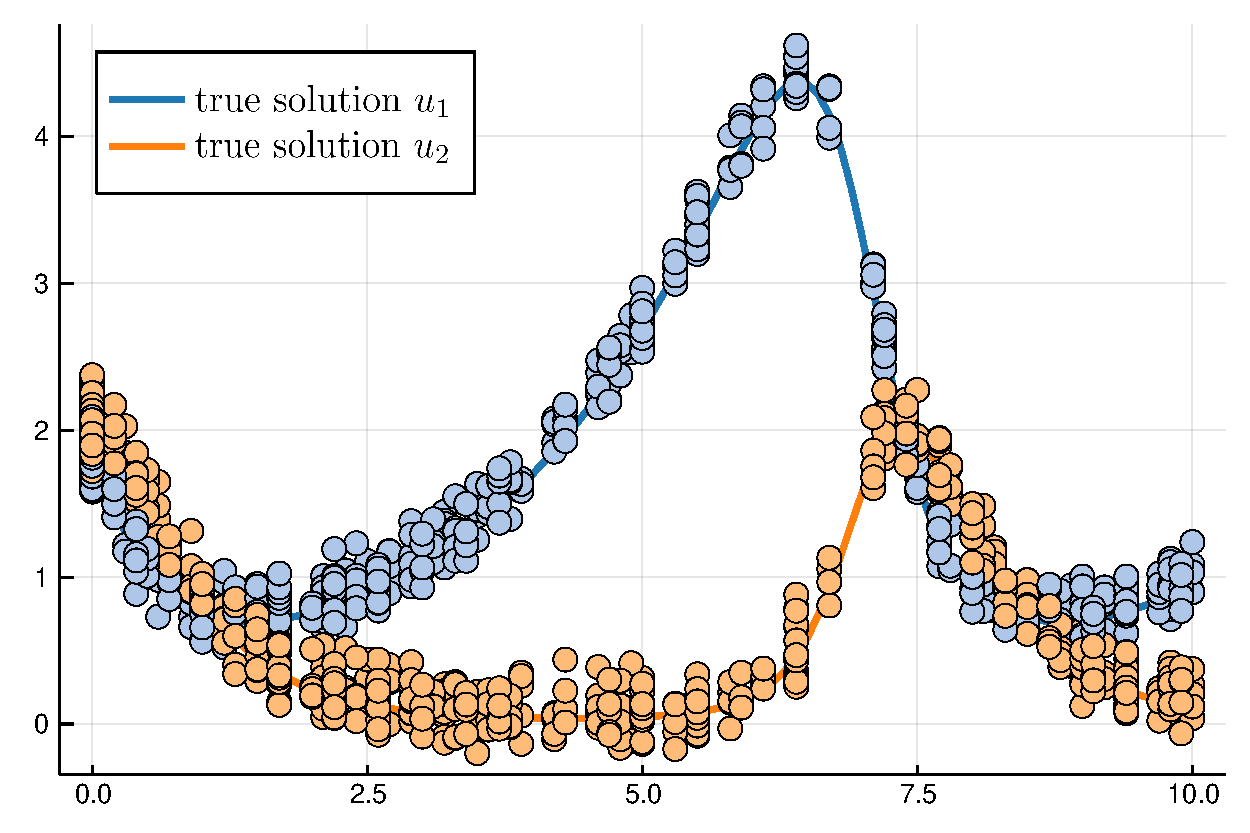
\includegraphics[width=\linewidth]{data_true_solution_2_lv.pdf}
	\end{minipage}\begin{minipage}{.5\linewidth}
		\centering
		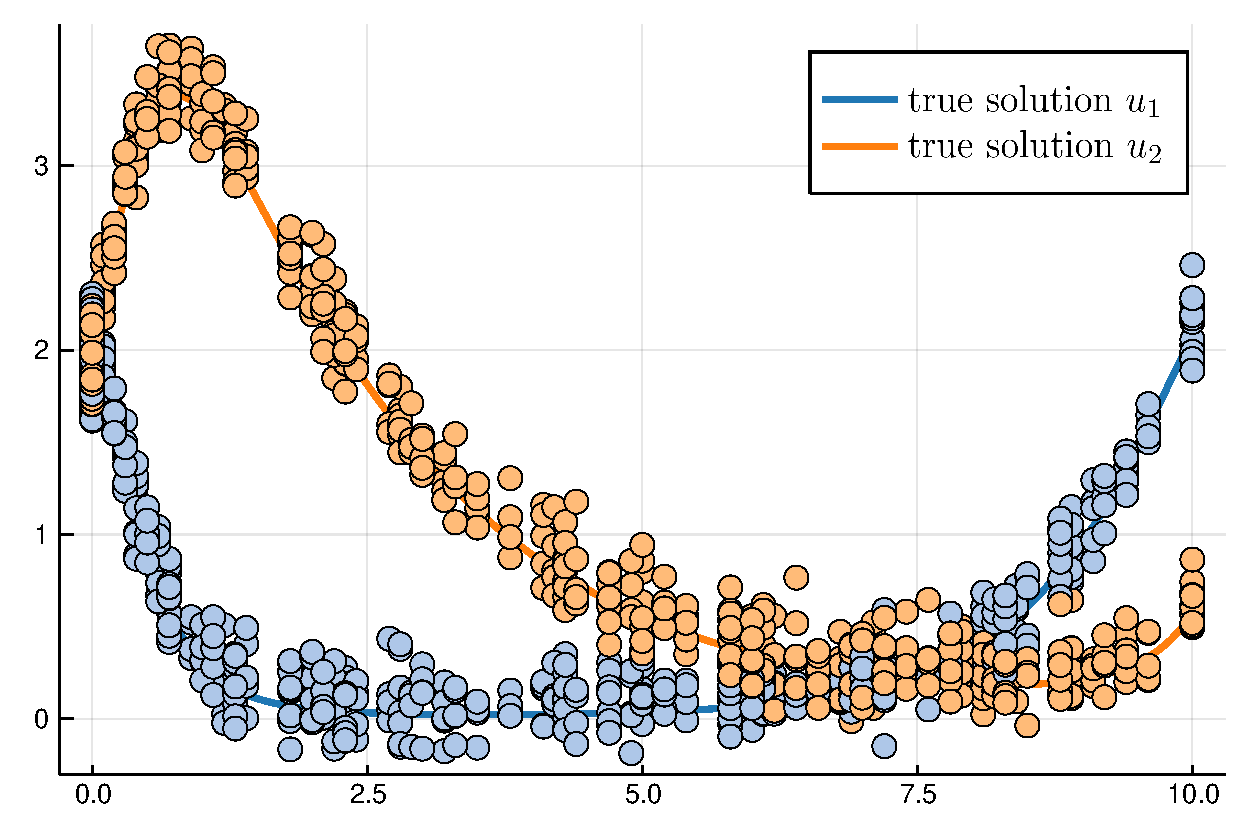
\includegraphics[width=\linewidth]{data_true_solution_1_lv.pdf}
	\end{minipage}
	\caption{Simulated observations of $200$ individuals ($100$ in each group) at $t_0$ and an individual-specific time point $t_1^i$.}
	\label{fig:data_truesolution_lv}
\end{figure}

\subsection{Individual fitted ODE solutions}\label{sec:apps-nonlinear2p-individualresults}

On these simulated data, the ODE-VAE model is trained to estimate the two parameters that differ between the two ODE systems, i.e., the parameters $\beta$ and $\delta$ from (\ref{eq:general-lotka-volterra-system}) describing the interaction of the two components are set to the true value of $1$ and the model learns the two other parameters $\alpha$ and $\gamma$. Thus, for each individual $i$, the initial value problem 
	\begin{equation*}
		\begin{split}
			\frac{d}{dt}\mu_1(t) &= \eta_{i,1} \mu_1(t) - \mu_1(t) \mu_2(t), \\
			\frac{d}{dt}\mu_2(t) &= \mu_1(t) \mu_2(t) - \eta_{i,2} \mu_1(t); \\
			\mu_{i}(t_0) &= \mu_{i}\tn 
\end{split}
\end{equation*}
is solved in latent space at the individual's second measurement time point $t_i^1$ with the ODE-net outputs $\eta_{i,1}, \eta_{i,2}$. 

In this setting, we first look at fitted ODE solutions for selected individuals and compare the two groups of underlying development patterns. For this application, I simulate baseline variables based on the true ODE parameters as in Algorithm~\ref{algo-simulation-baseline-trueODEparams} and set $\sigma_{\mathrm{info}} = \sigma_{\mathrm{noise}} = 0.5$ and $q_{\mathrm{info}}= 30$, i.e., simulate $30$ variables containing the respective baseline information and add $20$ noise variables. Then, I train the model for $40$ epochs with the ADAM SGD-optimiser and a learning rate of $0.0001$. 
\begin{figure}
	\centering
	\begin{minipage}{\linewidth}
		\begin{minipage}{.5\textwidth}
			\centering				
			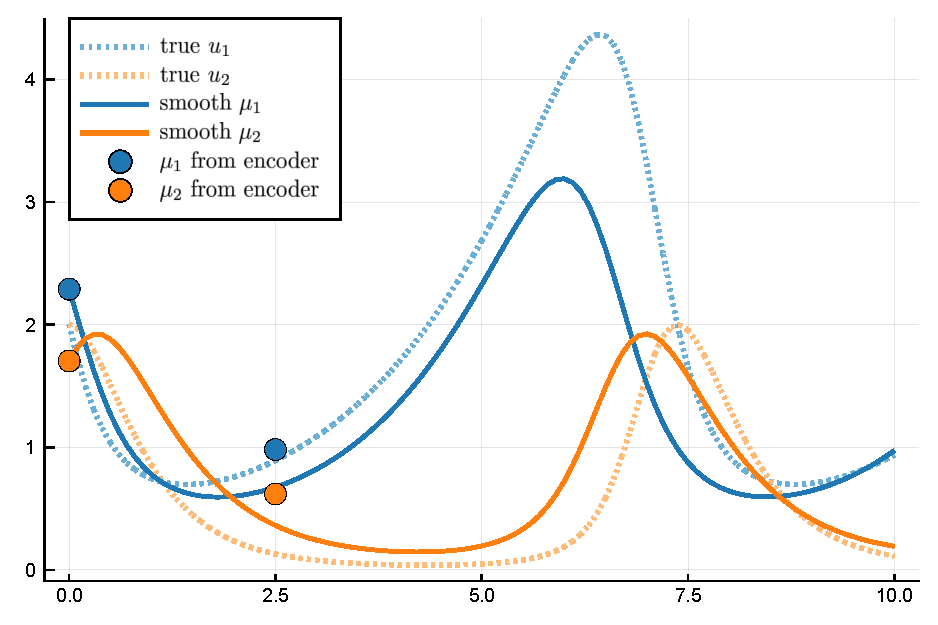
\includegraphics[width=\linewidth]{z_trajectory_plots_2ps_lv_1early.pdf}
		\end{minipage}\begin{minipage}{.5\textwidth}
			\centering
			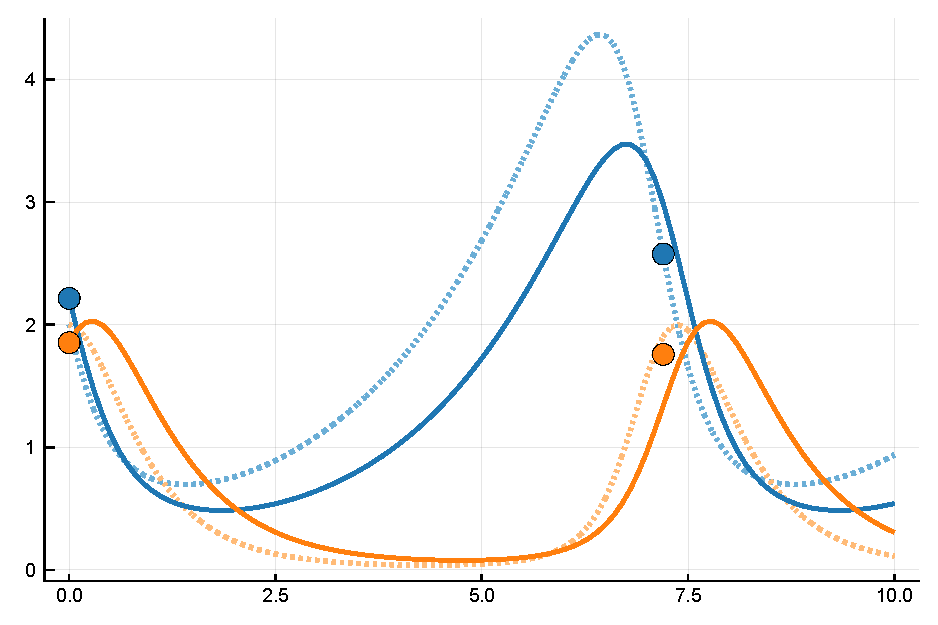
\includegraphics[width=\linewidth]{z_trajectory_plots_2ps_lv_1late.pdf}
		\end{minipage}
	\end{minipage}
	\begin{minipage}{\linewidth}
		\begin{minipage}{.5\textwidth}
			\centering
			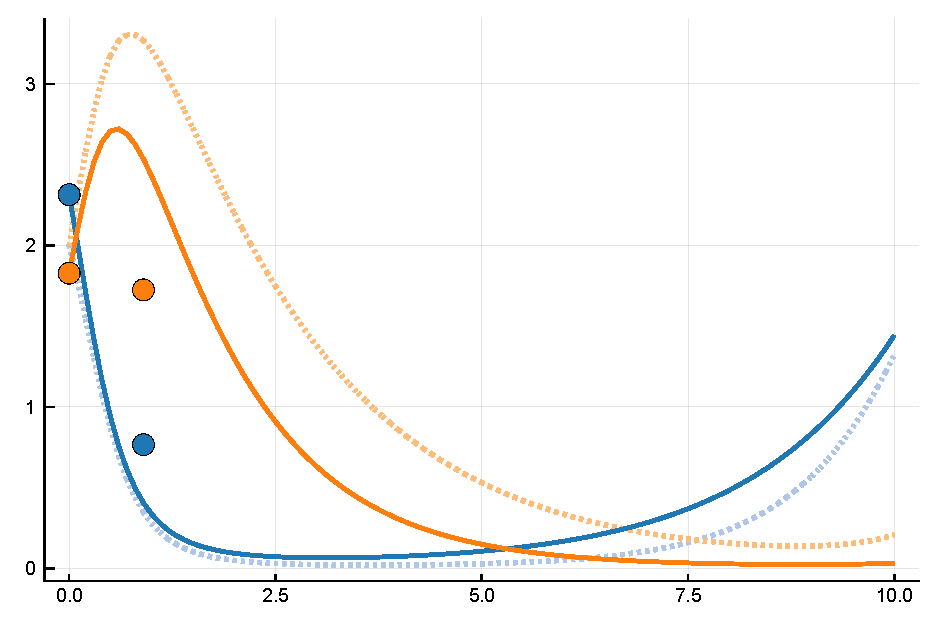
\includegraphics[width=\linewidth]{z_trajectory_plots_2ps_lv_2early.pdf}
		\end{minipage}\begin{minipage}{.5\textwidth}
			\centering
			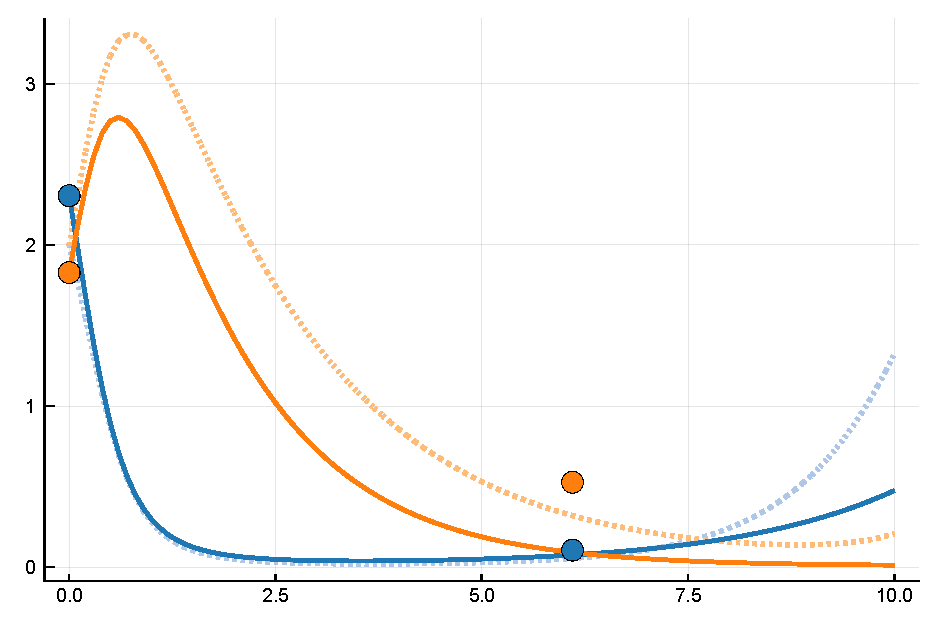
\includegraphics[width=\linewidth]{z_trajectory_plots_2ps_lv_2late.pdf}
		\end{minipage}
	\end{minipage}
	\caption{Fitted ODE solutions of four individuals with true ODE parameters as baseline information: Two individuals from each group are shown, one with a second measurement time point rather at the beginning of the time interval (left column) and one with a rather late simulated second measurement (right column).}
	\label{fig:apps_individual_solutions_tp_lv}
\end{figure}

Figure~\ref{fig:apps_individual_solutions_tp_lv} shows the fitted ODE solutions of four individuals.
Generally, the model learns the structure of the underlying patterns in both groups. 
It slightly overestimates the initial value of the first component of the solution and slightly underestimates it in the second component. 
Comparable to the linear setting where the model tends to underestimate the upward trend, in this scenario the model also underestimates the high peaks of the first component $u_1$ for the first underlying pattern and of the second component $u_2$ in the second underlying pattern. 
At the peak of the second component in the left panel of the second row, the model has difficulty matching the mean obtained directly from the encoder (orange dot) to the trajectory of the mean obtained from solving the ODE (solid orange line). As in the linear case, this could be explained by the regularising effect of the $\mathcal{N}(0,I)$-prior on the fitted model posterior and the fact that the true trajectory is rather steep around the peak, such that the data from this region is not dense enough to sufficiently encourage the model to move the posterior to more extreme values away from the prior. 
As the encoder part of the VAE outputting the posterior means before solving the ODE has no access to the baseline variables containing information about the true parameters governing the ODE system, this phenomenon is less pronounced for the mean obtained as ODE solution which can be influenced by the baseline information. 

For the individual from the second group with a late second time point (right panel in second row), the mean from the VAE encoder before solving the ODE in the second component (orange dot) more closely matches the true trajectory (dotted orange line) than the fitted ODE solution (solid orange line). This tendency, albeit less evident, can also be observed for the first component of the mean from the VAE encoder in the both individuals from the first group (blue dots in the panels in the first row) and for the individual with a late second time point also in the second component (orange dot in the right panel of the first row). 
Probably related to the rather low level of noise in the simulated data, the model thus tends to fit a more data-oriented representation of the mean before solving the ODE. This gets more difficult if there is no sufficient data, in which case the regularising $\mathcal{N}(0,I)$-prior gains influence, as for the second mean component in the left panel in the second row.  
Generally, also in the non-linear case the basic distinct trends in the developments are captured and reflected by both the ODE solutions and the means from the VAE encoder. 

\subsection{Training with different numbers of informative baseline variables}\label{sec:apps-nonlinear2p-diffbaselinenumbers}
The aim of this section is to investigate the effect of the numbers of infomative and noise variables at $t_0$. To visualise the variability of the results across the entire dataset and to be able to evaluate the effect of more or less informative baseline variables on the overall model performance, I overlay the fitted ODE solutions of all individuals from each of the two groups and their posterior means from the VAE encoder as in Figures~\ref{fig:apps_allinds_comparison_tp_gi_2pslinear} or \ref{fig:apps_allinds_comparison_morelessnoise_bothgroups_linear}. I conduct four training runs with a different number of informative baseline variables with the time-dependent data described in Section~\ref{sec:apps-nonlinear-inputdata} (Figure~\ref{fig:data_truesolution_lv}). Specifically, I set $q_{\mathrm{info}} = 10, 20, 30, 40$ and for each setting, simulate the baseline information based on the true ODE parameters and the noise variables as described in Algorithm~\ref{algo-simulation-baseline-trueODEparams} with $\sigma_{\mathrm{info}} = \sigma_{\mathrm{noise}} = 0.5$. 
I keep all hyperparameters fixed across the four training runs and always start with the same initialisation of the model weights and biases. As in the previous Section~\ref{sec:apps-nonlinear2p-individualresults}, in each setting, the model is trained for $40$ epochs with the ADAM-optimiser and a learning rate of $0.0001$ without individual tuning of hyperparameters.  
Figure~\ref{fig:apps_allindsoverlaid_diffnobaselines} shows the resulting fitted ODE solutions. 
\begin{figure}
	\centering
	\begin{minipage}{\linewidth}
		\begin{minipage}{.5\textwidth}
			\centering				
			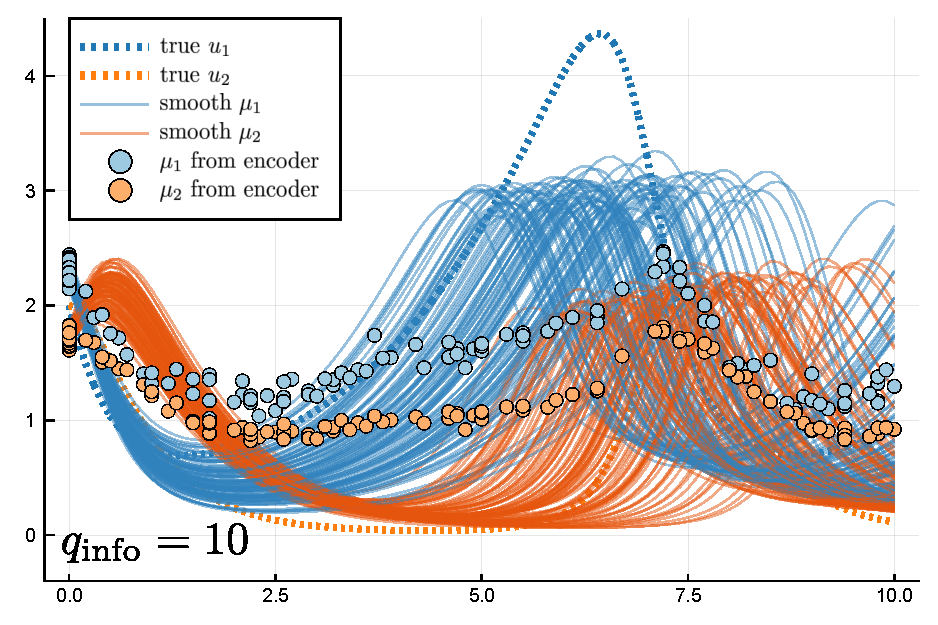
\includegraphics[width=\linewidth]{10inforvars_allindsoverlaid_2.pdf}
		\end{minipage}\begin{minipage}{.5\textwidth}
			\centering
			\vspace{4.2pt}
			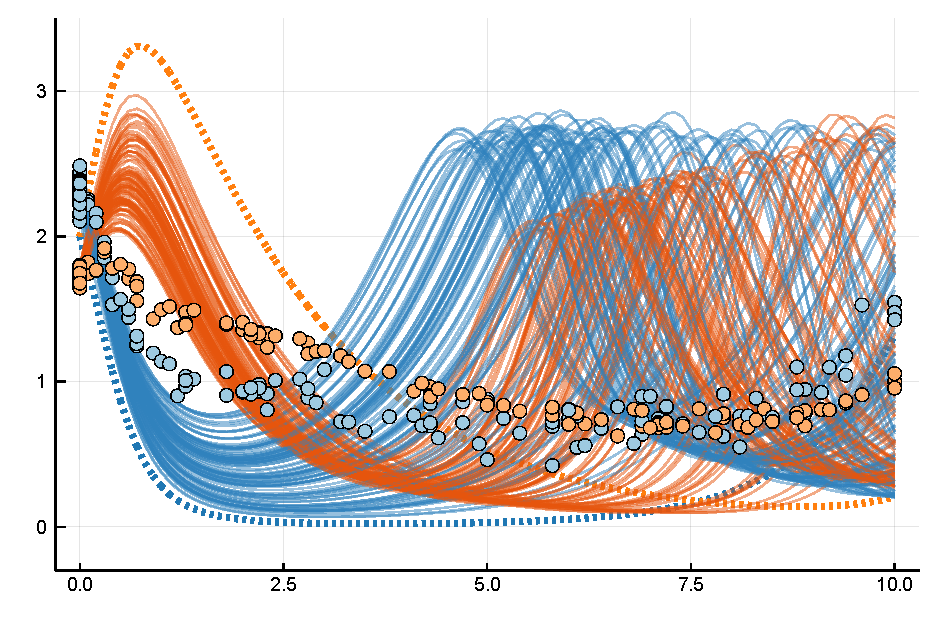
\includegraphics[width=\linewidth]{10inforvars_allindsoverlaid_1.pdf}
		\end{minipage}
	\end{minipage}
	\begin{minipage}{\linewidth}
		\begin{minipage}{.5\textwidth}
			\centering				
			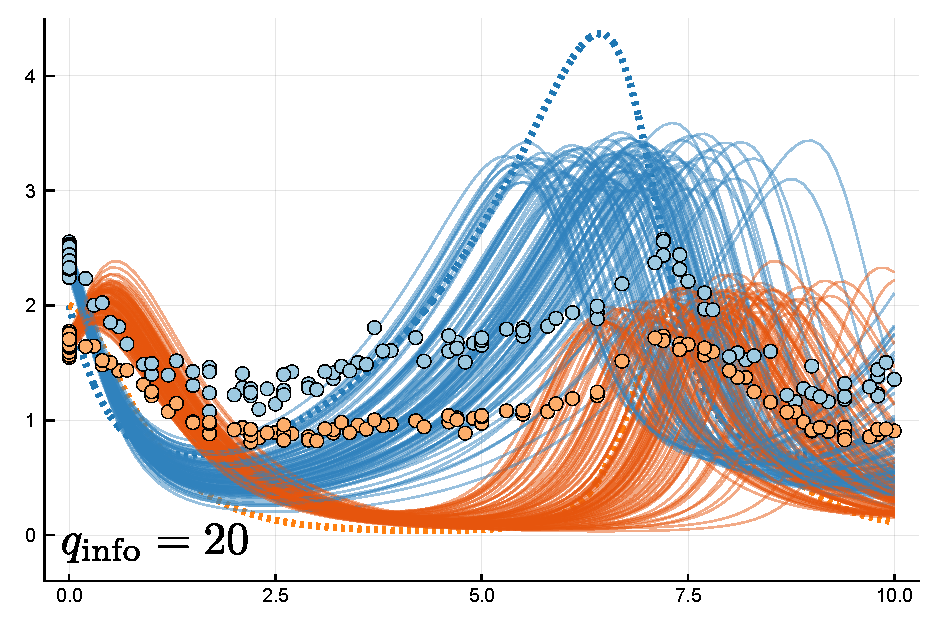
\includegraphics[width=\linewidth]{20inforvars_allindsoverlaid_2.pdf}
		\end{minipage}\begin{minipage}{.5\textwidth}
			\centering
			\vspace{4.2pt}
			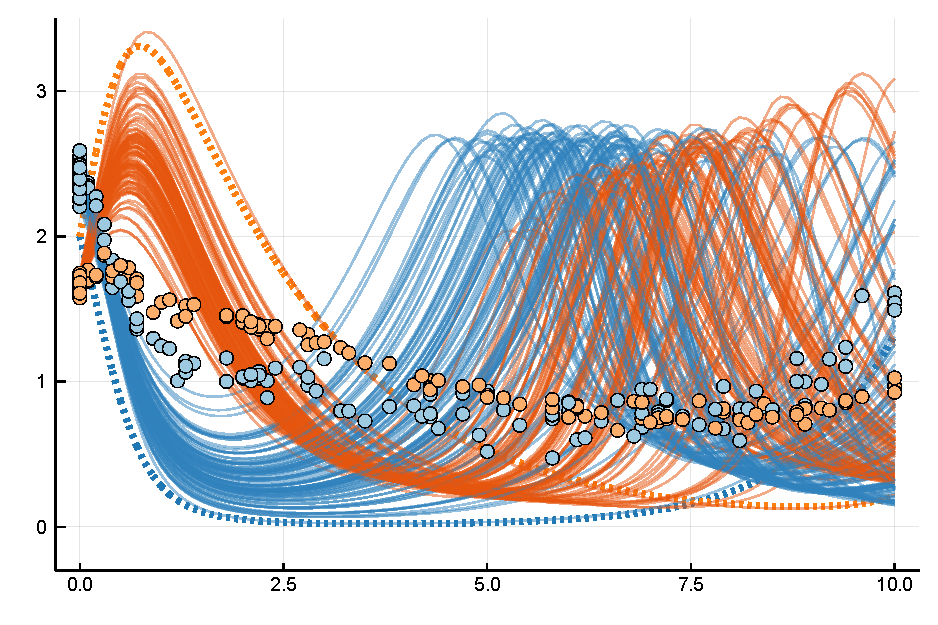
\includegraphics[width=\linewidth]{20inforvars_allindsoverlaid_1.pdf}
		\end{minipage}
	\end{minipage}	
	\begin{minipage}{\linewidth}
		\begin{minipage}{.5\textwidth}
			\centering				
			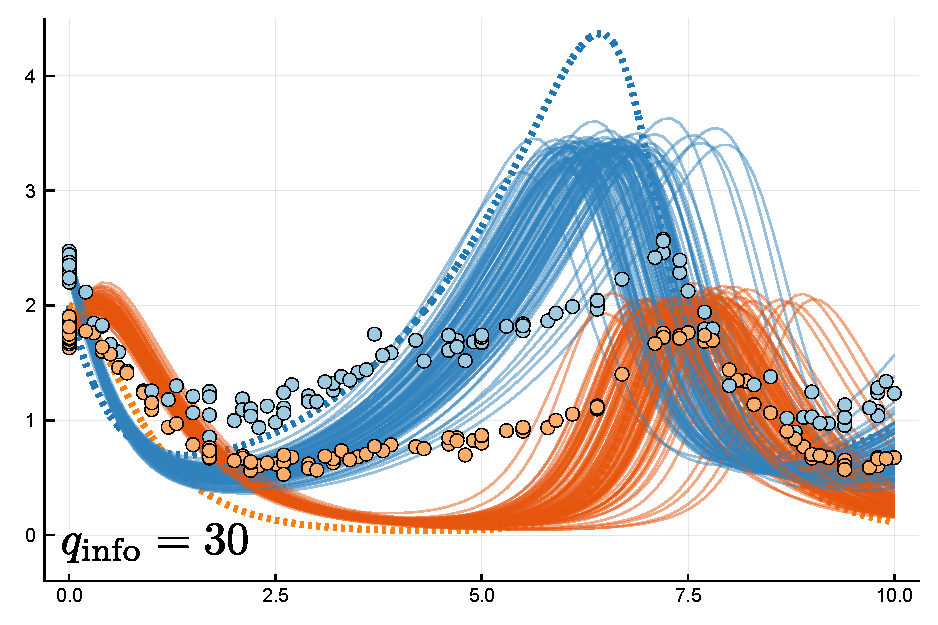
\includegraphics[width=\linewidth]{30inforvars_allindsoverlaid_2.pdf}
		\end{minipage}\begin{minipage}{.5\textwidth}
			\centering
			\hspace*{4pt}
			\vspace*{4.2pt}
			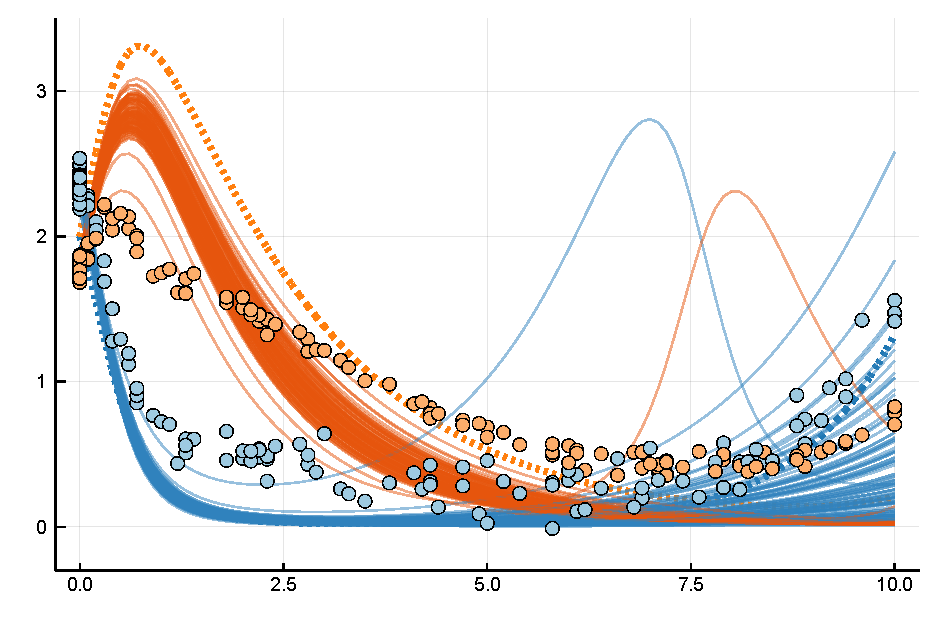
\includegraphics[width=\linewidth]{30inforvars_allindsoverlaid_1.pdf}
		\end{minipage}
	\end{minipage}
	\begin{minipage}{\linewidth}
		\begin{minipage}{.5\textwidth}
			\centering				
			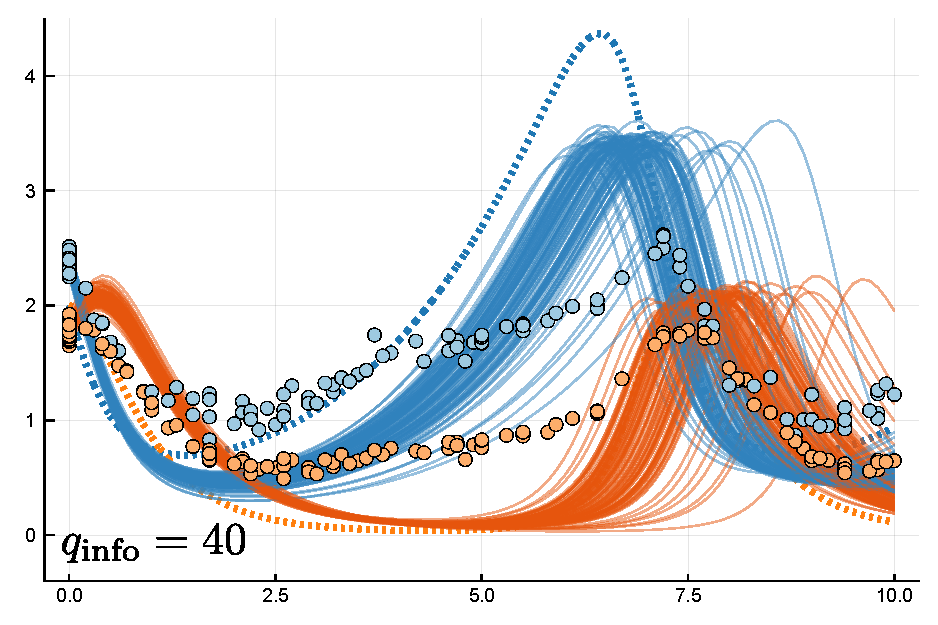
\includegraphics[width=\linewidth]{40inforvars_allindsoverlaid_2.pdf}
		\end{minipage}\begin{minipage}{.5\textwidth}
			\centering
			\vspace{4.2pt}
			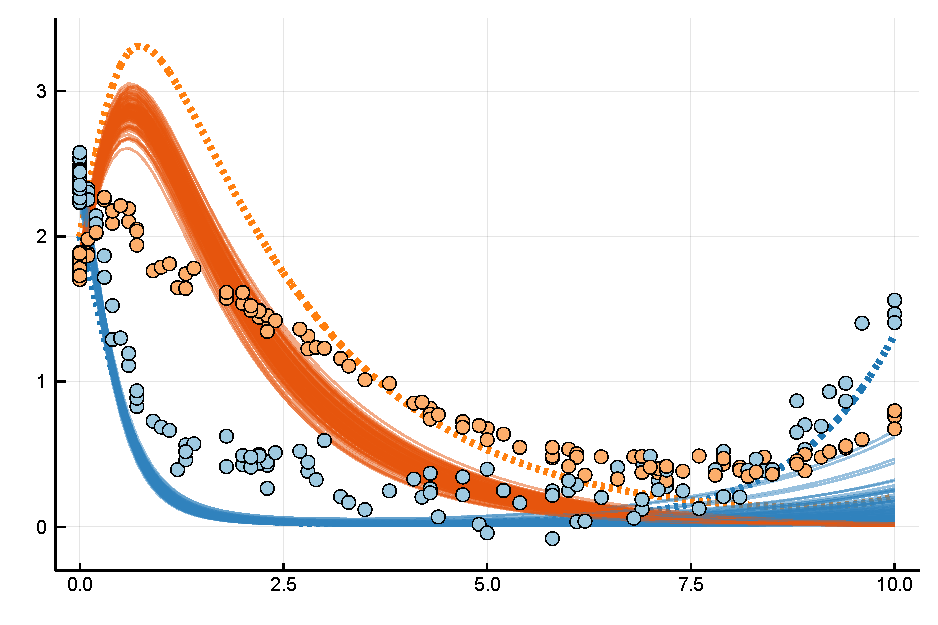
\includegraphics[width=\linewidth]{40inforvars_allindsoverlaid_1.pdf}
		\end{minipage}
	\end{minipage}
	\caption{Comparison of all individuals' fitted ODE solutions for different baseline variables based on the true ODE parameters. One panel shows the solutions of all individuals from one group of underlying development patterns. One row of panels belongs to one training run with the indicated number of informative baseline variables.}
	\label{fig:apps_allindsoverlaid_diffnobaselines}
\end{figure}

In the first two rows corresponding to the training results with $10$ and $20$ baseline variables carrying information about the true ODE parameters, the model has difficulty inferring the distinct group-specific ODE parameters, as the fitted ODE solutions of both groups are more similar than the actual ground-truth trajectories. While the first underlying pattern is essentially recognised by the model, although with substantial variability, the second underlying ground-truth pattern (right column) is not captured well: The peaks that the model generates in the solutions will in fact also appear in the ground truth solution (due to its periodicity), but at a later time point outside the depicted time interval, indicating that the model underestimates the length of the period of the solution and hence does not infer the correct parameters of the system. 

Additionally, in the first two rows, the model again underestimates the peaks both of the first solution component for the first group of individuals (left column) and of the second solution component in the second group of individuals (right column). With $20$ baseline variables, the model matches the peaks a bit better, reinforcing our previous observation that a lower level of noise helps the model to fit a posterior closer to the data and further away from the $\mathcal{N}(0,I)$-prior.  

Interestingly, in these first two scenarios, the means from the VAE encoder before solving the ODE actually describe the ground truth trajectories better than the fitted ODE solutions and, unlike them, do reflect the different underlying development patterns in the data. 
With $30$ out of $50$ baseline variables carrying information, the model also recovers the second underlying pattern in the fitted ODE solutions. The variability between individuals in both groups is strongly reduced in comparison to the setting with only $10$ informative baseline variables. There is also less variability in the means from the encoder and they better match the ODE solution, although the improvement in performance with respect to the means from the encoder is not as pronounced as for the fitted ODE solutions. 
This is hardly surprising as the VAE encoder is not directly influenced by the baseline information and hence not as sensitive to a higher level of noise in them as the fitted ODE solutions that depend directly on the ODE parameters inferred from the baseline variables. Rather, the fact that they do improve at all confirms again that our training objective of bringing these posterior means from before and after solving the ODE together can successfully guide the model towards finding a meaningful, consistent latent representation and ODE parameters that fit the data.

This becomes evident particularly in the second group of individuals (right column): In the first two rows, where the encoder means describe the ground truth trajectories better than the fitted ODE solutions, there is not much change between $10$ and $20$ informative baseline variables. However, for $30$ baseline variables carrying information, the fitted ODE solutions reflect the underlying true pattern, and also the improvement in the fit of the encoder means is larger than before. Both mean representations are subject to a lower level of variability between individuals and in both components, the means from the encoder match both the ground truth and the fitted ODE solutions much better. This implies that more baseline information helps the VAE to find a better fitting ODE system, and a better fitting ODE system in latent space in turn helps the VAE to find a good latent representation that matches such a smooth development according to the ODE system already as direct output of the encoder, even before solving the ODE. 
In the last row corresponding to the results with $40$ informative baseline variables, compared to the results for $30$ informative baseline variables, mainly the variability across the dataset is further reduced. Even in this last setting, however, the model does not fit the peak of the first solution component in the first group of individual (solid blue lines in left panel) perfectly, and the means from the encoder (blue dots) underestimate it more significantly. In the second component, the means from the encoder do not match the ground-truth trajectory exactly, but still reflect the general non-linear structure. 

When performing the same experiments in the second simulation scenario of baseline variables, i.e., with only the information about the group membership (see Algorithm~\ref{algo-simulation-baseline-groupinfo}), I obtained much better fitting ODE solutions for low numbers of informative baseline variables (see Figure~\ref{fig:apps_allindsoverlaid_diffnobaselines_groupinfo}). Even with only $10$ informative baseline variables and despite the generally more difficult scenario of simulated baseline information, the model still clearly distinguishes the two development patterns and fits them with as little variability as in the setting with the true ODE parameters as baseline information and $30$ informative baseline variables. 
A possible explanation for this phenomenon might be that it can be easier for the model to distinguish between two groups if only the group membership is encoded in the baseline information: With the true ODE parameters as information, it has to take an additional step, i.e., it has to both infer the true parameters from the noisy information and then infer from that there are two groups, while with only the group membership, it is easier for the model to infer the general presence of two distinct groups from the data. 
As in the setting shown in Figure~\ref{fig:apps_allindsoverlaid_diffnobaselines_groupinfo}, the variability between individuals further decreases for an increased number of informative variables and the model generally has difficulty matching the means from the encoder and the means after solving the ODE in the regions of high peaks in the data. 

\begin{figure}
	\centering
	\begin{minipage}{\linewidth}
		\begin{minipage}{.5\textwidth}
			\centering				
			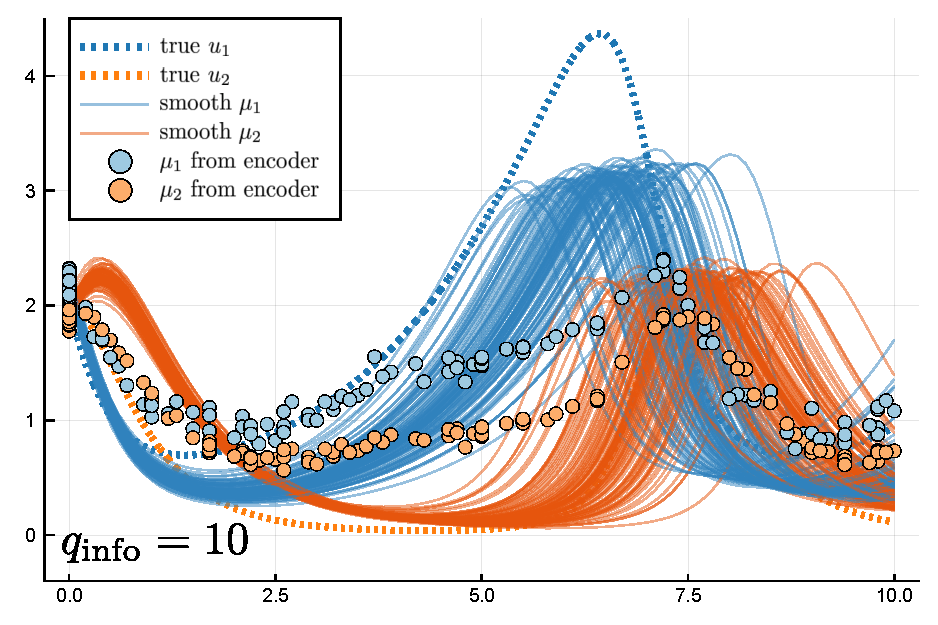
\includegraphics[width=\linewidth]{10inforvars_allindsoverlaid_groupinfo_2.pdf}
		\end{minipage}\begin{minipage}{.5\textwidth}
			\centering
			\vspace{4.2pt}
			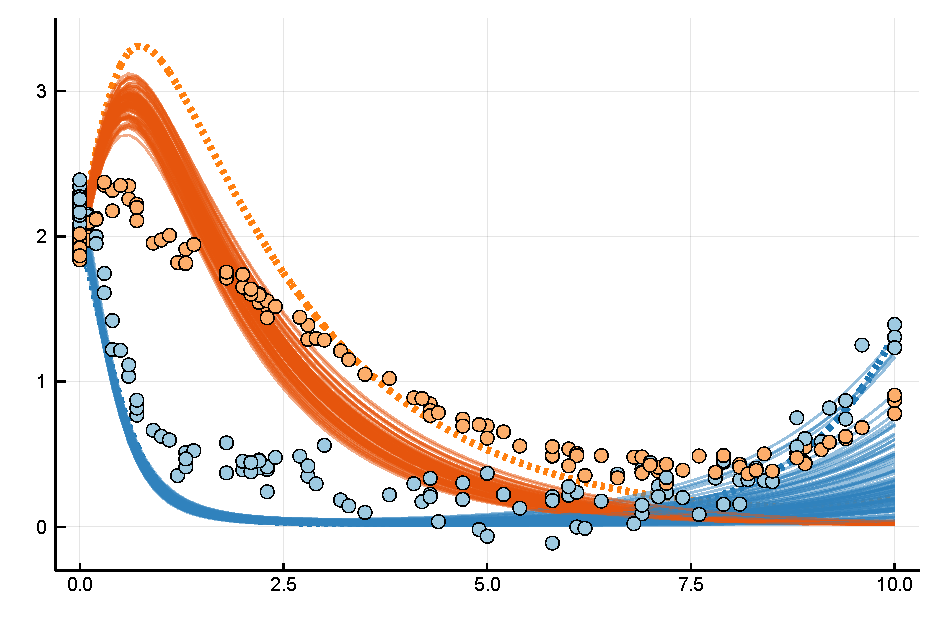
\includegraphics[width=\linewidth]{10inforvars_allindsoverlaid_groupinfo_1.pdf}
		\end{minipage}
	\end{minipage}
	\begin{minipage}{\linewidth}
		\begin{minipage}{.5\textwidth}
			\centering				
			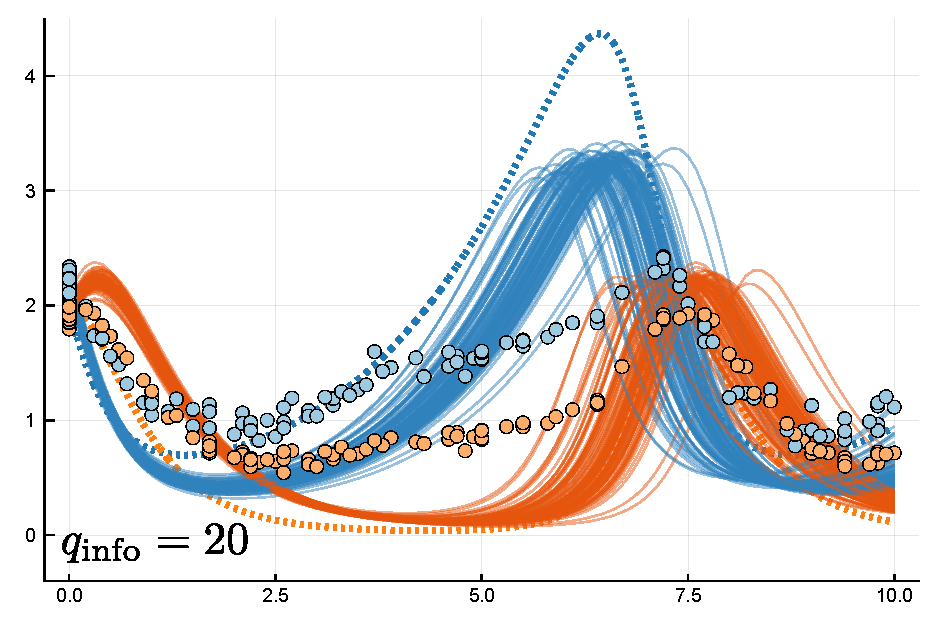
\includegraphics[width=\linewidth]{20inforvars_allindsoverlaid_groupinfo_2.pdf}
		\end{minipage}\begin{minipage}{.5\textwidth}
			\centering
			\vspace{4pt}			
			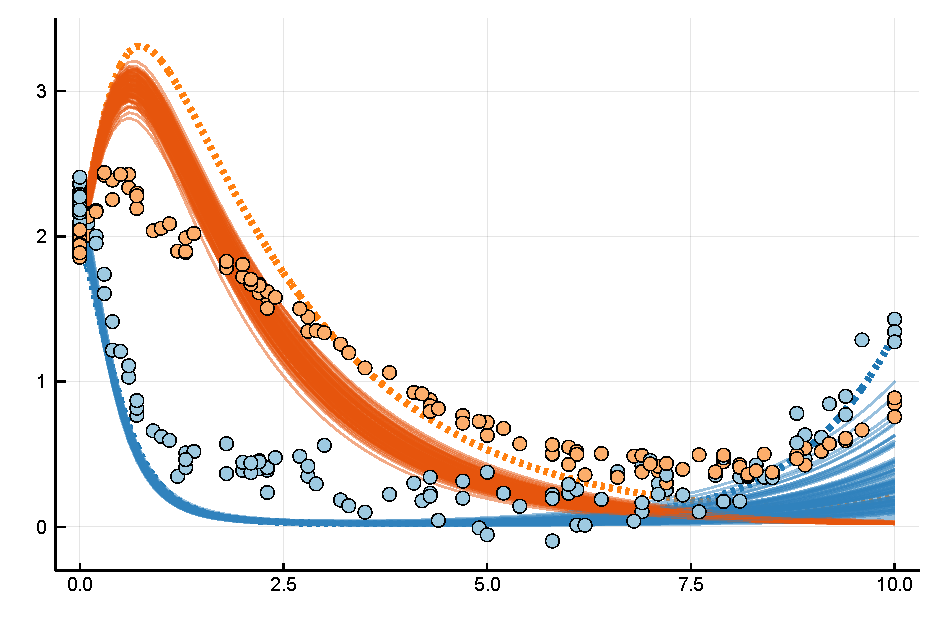
\includegraphics[width=\linewidth]{20inforvars_allindsoverlaid_groupinfo_1.pdf}
		\end{minipage}
	\end{minipage}	
	\begin{minipage}{\linewidth}
		\begin{minipage}{.5\textwidth}
			\centering				
			\includegraphics[width=\linewidth]{30inforvars_allindsoverlaid_groupinfo_2.pdf}
		\end{minipage}\begin{minipage}{.5\textwidth}
			\centering
			\hspace*{1pt}
			\includegraphics[width=\linewidth]{30inforvars_allindsoverlaid_groupinfo_1.pdf}
		\end{minipage}
	\end{minipage}
	\begin{minipage}{\linewidth}
		\begin{minipage}{.5\textwidth}
			\centering				
			\includegraphics[width=\linewidth]{40inforvars_allindsoverlaid_groupinfo_2.pdf}
		\end{minipage}\begin{minipage}{.5\textwidth}
			\centering
			\vspace{4.5pt}
			\includegraphics[width=\linewidth]{40inforvars_allindsoverlaid_groupinfo_1.pdf}
		\end{minipage}
	\end{minipage}
	\caption{Comparison of all individuals' fitted ODE solutions for different baseline variables based on the group membership. One panel shows the solutions of all individuals from one group of underlying development patterns. One row of panels belongs to one training run with the indicated number of informative baseline variables.}
	\label{fig:apps_allindsoverlaid_diffnobaselines_groupinfo}
\end{figure}

\section{Linear ODE system with four unknown parameters}\label{sec:apps-linear4p}

While the applications presented so far have covered settings where the number of parameters was equal to the number of simulated measurement time points, I now investigate the capability of the ODE-VAE model to fit more parameters in order to model more complex dynamical systems. In the following section, I therefore apply the extension of our training procedure described in Section~\ref{sec:methods-minibatches} and infer batches of individuals with similar trajectories to enrich individual's observations with proxy information at more time points from other individuals in the batch. 

\subsection{Structure of input data}

The model is trained on data from a linear ODE system as in Section~\ref{sec:apps-linear2p} and all four ODE parameters are estimated as outputs of the ODE-net. Again, two distinct underlying development patterns are defined as solutions of the ODE systems in Equations (\ref{eq:ODE-systems-4pslinear-1}) and (\ref{eq:ODE-systems-4pslinear-2}) and visualised in Figure~\ref{fig:apps-true_solution_linear_4ps}, similar to those in Section~\ref{sec:apps-linear2p-inputdata}. 

\begin{figure}
	\centering
	\begin{minipage}{.5\linewidth}
		\centering
		\includegraphics[width=\linewidth]{true_solution_2_4ps_linear.pdf}
		\scriptsize
		\begin{equation}\label{eq:ODE-systems-4pslinear-1}
		\begin{split}
		\frac{d}{dt}\begin{pmatrix} u_1 \\ u_2 \end{pmatrix}(t) &= \begin{pmatrix} -0.2 & 0.1 \\ -0.1 & 0.25 \end{pmatrix} \begin{pmatrix} u_1 \\ u_2 \end{pmatrix}(t); \\
		\begin{pmatrix} u_1 \\ u_2 \end{pmatrix}(0) &= \begin{pmatrix} 4 \\ 2 \end{pmatrix}
		\end{split}
		\end{equation}
		\normalsize
	\end{minipage}\begin{minipage}{.5\linewidth}
		\centering
		\includegraphics[width=\linewidth]{true_solution_1_4ps_linear.pdf}
		\scriptsize		
		\begin{equation}\label{eq:ODE-systems-4pslinear-2}
		\begin{split}
		\frac{d}{dt}\begin{pmatrix} u_1 \\ u_2 \end{pmatrix}(t) &= \begin{pmatrix} -0.2 & 0.1 \\ 0.1 & -0.2 \end{pmatrix} \begin{pmatrix} u_1 \\ u_2 \end{pmatrix}(t); \\
		\begin{pmatrix} u_1 \\ u_2 \end{pmatrix}(0) &= \begin{pmatrix} 4 \\ 2 \end{pmatrix}
		\end{split}
		\end{equation}
		\normalsize
	\end{minipage}
	\caption{True underlying development patterns characterised as solutions of two-dimensional linear ODE systems.}
	\label{fig:apps-true_solution_linear_4ps}
\end{figure}

%As in the previous sections, we simulate our data by drawing measurement points from these true trajectories and adding random noise as described in Algorithm~\ref{algo-simulation-time-dependent}. 
As in Section~\ref{sec:apps-linear2p-inputdata}, I generate observations of $10$ variables for $100$ individuals, $50$ from each of the two groups, by adding variable-specific and the individual-specific measurement errors to $5$ values from each of the two ODE solution components both at the initial time point $t_0 = 0$ and the second time point $t_1^i$ drawn uniformly from the interval $[1.5, 10]$ as in Algorithm~\ref{algo-simulation-time-dependent}. For this setting with four unknown parameters, I set $\sigma_{\mathrm{var}}= 0.1$ and $\sigma_{\mathrm{ind}} = 0.5$. Figure~\ref{fig:apps-data_truesolution_4ps_linear} visualises all simulated observations together with the true ODE solutions.
\begin{figure}
	\centering
	\begin{minipage}{.5\linewidth}
		\centering
		\includegraphics[width=\linewidth]{data_true_solution_2_4ps_linear.pdf}
	\end{minipage}\begin{minipage}{.5\linewidth}
		\centering
		\includegraphics[width=\linewidth]{data_true_solution_1_4ps_linear.pdf}
	\end{minipage}
	\caption{Simulated observations of $100$ individuals ($50$ in each group) at $t_0$ and an individual-specific time point $t_1^i$.}
	\label{fig:apps-data_truesolution_4ps_linear}
\end{figure}

\subsection{Comparison of different simulation scenarios of baseline variables}

On these data, the ODE-VAE model is trained as described in Chapter~\ref{chap:methods}, Section~\ref{sec:methods-minibatches} and Algorithm~\ref{algo-batches}. Specifically, all four parameters of each of the two ODE systems are estimated and in latent space, for each individual $i$ the initial value problem 
\begin{equation*}
	\begin{split}
		\frac{d}{dt} \mu_i(t) &= \begin{pmatrix} \eta_{i,1} && \eta_{i,2} \\ \eta_{i,3} && \eta_{i,4}	\end{pmatrix} \begin{pmatrix} \mu_{i,1} \\ \mu_{i,2}	\end{pmatrix} (t); \\
		\mu_i(t_0) &= \mu_i\te
	\end{split}
\end{equation*}
is solved at the individual's second time point $t_i^1$ with the ODE-net outputs $\eta_{i,1}, \dots, \eta_{i,4}$. 

As in Section~\ref{sec:apps-linear2p-comparisonbaseline}, the different simulations scenarios of baseline variables described in Algorithms~\ref{algo-simulation-baseline-trueODEparams} and \ref{algo-simulation-baseline-groupinfo} are compared. For the first scenario with the true ODE parameters, I set $\sigma_{\mathrm{info}} = \sigma_{\mathrm{noise}} = 0.1$ and for the second scenario with the group membership, I set $\sigma_{\mathrm{info}} = \sigma_{\mathrm{noise}} = 0.5$. In each scenario, I simulate $20$ variables containing the respective baseline information, add $30$ noise variables and train the model for $15$ epochs with the ADAM SGD-optimiser and a learning rate of $0.001$. 

Empirically, I found that for my setting with two distinct underlying patterns, a small batchsize ($b \leq 5$) is insufficient to capture the complete dynamics because it provides too little time points and proxy observations. On the other hand, a large batchsize with respect to the dataset size ($b \gg \frac{n}{10}$) introduces training instability due to too many individuals with different development pattern being grouped together.
Between those extremes, I found the results to be robust against different choices of batchsizes and present in the following only results for a batchsize of $b=10$. 

I also found that the results are stable with respect to different choices of kernel functions, including using equal weights for all individuals in the batch. 
In the more difficult scenario of using only the group membership as baseline information, however, the weighting approach does improve the model performance. Thus, I chose to use the kernel approach for all applications with the tricube function as kernel and a bandwidth of $1$ without tuning this hyperparameter.

Figure~\ref{fig:apps-comparison_tp_gi_individualbatches_linear4ps} compares the ODE solutions of individual minibatches for the two simulation scenarios of baseline variables. 

\begin{figure}
	\includegraphics[width=\linewidth]{comparison_baselinevars_individualsolutions_linear4ps.pdf}
	\caption{Comparison of fitted ODE solutions of selected minibatches for both scenarios of simulated baseline variables. One panel depicts the fitted ODE solutions of all individuals from one batch. Thick, dark lines and dots represent the latent representation means of the reference individual around which the batch was grouped, while lighter, thin lines and dots belong to the other individuals in the batch.}
	\label{fig:apps-comparison_tp_gi_individualbatches_linear4ps}
\end{figure}
Generally, we can see that the second measurement time points of all individuals in the batch do cover the entire time interval, and that all individuals in one batch share a common development trend in both components of the ODE solution.
For training with the group membership as baseline information, we observe the phenomenon mentioned in Section~\ref{sec:apps-linear2ps-trainingvariability} of the inverted signs of the initial condition and the model flipping the first component of the fitted solution at the $x$-axis. In both compared settings, the model again inverts the dimensions, i.e., fits the first component of the true ODE solution with the second component of its latent representation mean and vice versa. 

In the scenario with the true ODE parameters, the fitted ODE solutions show the correct trends of the ground-truth solutions, but, especially in the first component, underestimate the true solution. This is even more pronounced in the first component of the means obtained from the VAE encoder before solving the ODE. However, these means also reflect the true developments with some variability (the apparently higher variability in the second row is due to the different scaling of the axis). When trained with only the group membership as baseline information, the fitted ODE solutions vary more strongly between individuals from the batch, especially in the upper panel. Again, in particular the first component of the fitted ODE solution underestimates the true trend.

Figure~\ref{fig:apps-comparison_tp_gi_allinds_linear4ps} compares the results of all individuals from each of the two groups in the two simulation scenarios of baseline variables by overlaying all individual ODE solutions and encoder means from one group of underlying development patterns in one panel. In general, the variability between individual's solutions from the same group is higher with only the group membership as baseline information. In both scenarios, particularly the upward trend of the second ground-truth ODE solution component is underestimated, while the fitted ODE solutions show that the integrated ODE solving step can partially improve this. 
The variability of the means from the encoder tends to be higher later in the time interval, reflecting the greater uncertainty in the fitted ODE solutions at those later time points. While for the first scenario with the true ODE parameters, the general trends of the trajectories are still distinguishable, they become more and more masked by individual variability in the second scenario.
Our observations are thus generally similar to those for the linear system with only two unknown parameters, although there is more variability and in general a weaker signal present in the application with four unknown parameters. On the other hand, the underlying problem of inferring more parameters than observed time points is much more difficult.

Additionally, I investigated the use of randomly assigned minibatches without inferring individuals' similarity and training without the batches as in the previous sections. Here, I found that without any batches, the model is not able to identify two distinct development patterns at all, and has significantly more difficulty inferring the correct trends of the trajectories with random minibatches. 

Overall, although the results are subject to substantial variation for different initialisations of model weights and biases, the proposed method of training on batches can still enable the achievement of similar results to the two-parameter case in this substantially more difficult setting. 

\begin{figure}
	\includegraphics[width=\linewidth]{comparison_tp_gi_linear_4ps.pdf}
	\caption{Comparison of fitted ODE solutions of all individuals from both groups for both scenarios of simulated baseline variables.}
	\label{fig:apps-comparison_tp_gi_allinds_linear4ps}
\end{figure}

\chapter{Discussion}\label{chap:discussion}
\fancyhead[LO]{\nouppercase{\leftmark}}

In this thesis, I have adapted the architecture of the variational autoencoder, a generative deep learning framework, to develop a model that can identify the central factors of variation in temporal development patterns and recover them in a non-linear and unsupervised fashion. I have constrained the latent space to model smooth trajectories by integrating an ODE system and augmented the model with another neural network used to infer individual-specific ODE parameters from additional baseline variables.
Furthermore, I have extended the model to train on batches of similar individuals, using combined measurements of other individuals from the batch as proxy information on the common trajectory at multiple time points. 

Inspired by a data scenario from a NAKO sub study, I have devised a simulation design where data are generated from distinct underlying temporal developments with random measurement noise at a common baseline time point and an irregularly sampled individual second time point. Then, the model has been applied and evaluated on these simulated data from both a linear and a non-linear ODE system with two unknown parameters and trained on batches of similar individuals on data from a linear system with four unknown parameters. I have compared different simulation scenarios of baseline information and different numbers of informative baseline variables and investigated the model performance for different levels of simulated measurement noise and across several training runs.

Overall, it could be shown that the proposed ODE-VAE model can recover the distinct underlying development patterns and infer individual-specific ODE parameters in various simulated data settings and accurately identify groups of individuals with similar trajectories. In conclusion, it thus provides an individual-level understanding of the temporal dynamics underlying individuals' developments and, rather than estimating average effects, has the potential to plan interventions based on the knowledge of full individual-specific dynamical systems.

With respect to related research, the main novelties of my method are the employment of batches of similar individuals to get proxy information on additional measurement time points and training the model in an iterative expectation-maximisation-like procedure to be able to afford more ODE parameters and thus model more complex dynamics. Also, the idea to infer individual-specific ODE parameter sets from additional baseline information has been introduced. What further differentiates my approach from, e.g., the latent time-series models in \cite{Chen2018} and \cite{Rubanova2019} is solving the ODEs at the level of the latent representation and implicitly conditioning the smooth mean obtained from solving the ODE on the data from the second measurement time point by adapting the training objective to explicitly encourage consistency of the latent representation means before and after solving the ODE. 
 
The main limitations of the method are that some knowledge on the underlying dynamics is required to define the general structure and dimensionality of the ODE system and the general sensitivity of the model to noisy information in the time-dependent and baseline variables as well as to how the data is scaled with respect to the $\mathcal{N}(0,1)$-prior. Additionally, even for only moderately complex scenarios, the model performance is subject to substantial variability for different random initialisations of the model parameters. In its current form, the method is restricted to a rather specific setting. 

For future research, it would thus be promising to leverage the method to model more complex or higher-dimensional dynamical systems, possibly also with more measurement time points, and to more thoroughly investigate its performance by defining rigorous evaluation criteria and averaging over many training runs. Finally, it would be crucial to test and evaluate the model performance on real-world datasets such as the NAKO study, which could then guide the modelling of more complex scenarios based on results from real data once they become available.

\newpage

% Bibliography
\renewcommand{\bibname}{References}
\bibliographystyle{unsrt}
\bibliography{bibfile}

% Germany summary 
\chapter*{Zusammenfassung in deutscher Sprache}

%Biomedizinische Zeitreihendaten von Individuen sind oft durch ein dünn besetztes und unregelmäßiges Zeitraster von Messungen sowie durch unterschiedliche individuelle Entwicklungsmuster gekennzeichnet. Motiviert durch ein Szenario aus der epidemiologischen Studie der Deutschen Nationalen Kohorte (NAKO) und inspiriert von den jüngsten Fortschritten bei der Kombination von Black-Box-Deep Learning mit expliziter mechanistischer Modellierung durch Differentialgleichungen, entwickeln wir ein generatives Modell, das die individuelle Dynamik in einer niedrigdimensionalen latenten Darstellung als Lösungen von gewöhnlichen Differentialgleichungen (ODEs) erfasst.  
%Trotz des wachsenden Potenzials und der Nachfrage nach personalisierter Medizin fehlt es häufig an geeigneten Daten. Eine individualisierte Behandlung erfordert eine Charakterisierung der dynamischen Entwicklung jedes einzelnen Individuums im Laufe der Zeit, aber die Erfassung dichter Zeitreihendaten mit vielen Variablen, die zu mehreren Zeitpunkten gemessen werden, ist aufwändig. 

Bei der Betrachtung biomedizinischer Zeitreihendaten ist das Verständnis der zugrunde liegenden dynamischen Systeme auf individueller Ebene der erste und wesentliche Schritt für eine personalisierte Behandlung. Solche Daten weisen jedoch oftmals ein spärliches und unregelmäßiges Zeitraster von Messungen sowie individuell verschiedene Entwicklungen auf, was die Modellierung erschwert. 

In dieser Arbeit wird basierend auf einem generativen Deep Learning-Verfahren ein Modell entwickelt, das aus solchen spärlichen und unregelmäßig beobachteten Zeitreihendaten einen niedrigdimensionalen latenten Raum lernt, in dem die individuellen Entwicklungsmuster als Lösungen gewöhnlicher Differentialgleichungen repräsentiert werden. Meine Methodik ist dabei von aktuellen Forschungsarbeiten zur Kombination von Deep Learning-Verfahren mit einer expliziten mechanistischen Modellierung durch Differentialgleichungen inspiriert und durch ein Szenario aus der Nationalen Kohorte (NAKO), einer groß angelegten epidemiologischen Kohortenstudie, motiviert.

Basierend auf einer NAKO-Substudie simuliere ich Daten, die sich durch eine umfangreiche Charakterisierung jedes Individuums mit Messungen vieler Variablen zu einem Baseline-Zeitpunkt auszeichnen, wobei eine kleinere Teilmenge dieser Variablen zu einem zweiten, für jedes Individuum unterschiedlichen, Zeitpunkt erneut gemessen wird. Insgesamt liegen somit individuelle dynamische Prozesse vor, die nur selten (je zwei Zeitpunkte pro Individuum) und unregelmäßig mit einer gewissen Messunsicherheit beobachtet werden. 
Ziel meiner Arbeit ist es, in einem solchen Szenario ein Modell zu entwickeln, das trotz der Messfehler sowie des groben und unregelmäßigen Zeitrasters die zugrunde liegenden individuellen Entwicklungsmuster extrahieren kann. 

Hierbei verwende ich einen Variational Autoencoder (VAE), ein generatives Deep-Learning-Modell, um anhand der beobachteten Entwicklungsmuster in einem nichtlinearen, unüberwachten Lernverfahren einen niedrigdimensionalen latenten Raum abzuleiten, der die zentrale, den Daten zugrunde liegende Dynamik repräsentiert. Um glatte Trajektorien zu modellieren, wird der latente Raum auf einen Raum differenzierbarer Funktionen eingeschränkt, die als Lösungen eines vorab definierten ODE-Systems vorliegen. Basierend auf der Annahme, dass individuelle Unterschiede in den Entwicklungsmustern auf Unterschiede in den nur bei zum Baseline-Zeitpunkt gemessenen Variablen zurückgeführt werden können, verwende ich diese Baseline-Variablen, um mithilfe eines weiteren neuronalen Netzes individuelle ODE-Parameter zu bestimmen.

Um komplexere zugrunde liegende dynamische Systeme modellieren zu können, erweitere ich das Modell und bestimme für jedes Individuum eine Gruppe von Individuen mit ähnlichen Entwicklungsmustern. Die Kombination aller zweiten Messungen in der Gruppe dient dann als Proxy-Information für das betrachtete Individuum über die gemeinsame dynamische Entwicklung zu mehreren Zeitpunkten. Durch das Trainieren des Modells auf diesen Gruppen wird so die Unregelmäßigkeit der zweiten Messzeitpunkte ausgenutzt und die Information jedes einzelnen Individuums wird um zusätzliche, stellvertretende Informationen von anderen Individuen erweitert.
% und somit das Problem des dünnbesetzen Zeitgitters zu adressieren. 

In den Anwendungen auf die oben beschriebenen simulierte Daten konnte ich zeigen, dass das entwickelte Modell in der Lage ist, individuelle Entwicklungsmuster basierend auf linearen und nicht-linearen zweidimensionalen ODE-Systemen mit zwei oder vier unbekannten Parametern zu rekonstruieren und für ein gegebenes Individuum eine Gruppe von Individuen mit ähnlichen Entwicklungen zu ermitteln. 

Zusammenfassend bietet die vorgestellte Methode somit auf individueller Ebene Einsicht in die dynamischen Systeme, die den Entwicklungen verschiedener Individuen im Zeitverlauf zugrunde liegen, und kann die Planung personalisierter Interventionen anhand der Kenntnis solcher vollständigen individualspezifischen dynamischen Systeme ermöglichen.

\backmatter
\fancyhead[LO, RE]{Temporal Dynamics in Generative Models}

\end{document}